% =========================================================================
%  MAHROS -- IEEE journal-style paper
%  Build:  pdflatex main && pdflatex main
%  (references are pre-formatted in refs.tex; regenerate with
%   scripts/build_refs.py after editing references.bib)
% =========================================================================
\documentclass[journal]{IEEEtran}

\usepackage[T1]{fontenc}
\usepackage{amsmath,amssymb}
\usepackage{booktabs}
\usepackage{multirow}
\usepackage{array}
\usepackage{tabularx}
\usepackage[nocompress]{cite}
\usepackage{graphicx}
\usepackage{xcolor}
\usepackage{algorithm}
\usepackage{algpseudocode}
\usepackage{tikz}
\usetikzlibrary{arrows.meta,positioning,fit,calc,shapes.geometric,shapes.multipart,backgrounds}
\usepackage{pgfplots}
\pgfplotsset{compat=1.17}
\usepgfplotslibrary{groupplots}
\usepackage{url}
\usepackage[hidelinks]{hyperref}

% ---- house style -------------------------------------------------------
\newcommand{\mahros}{MAHROS}
\definecolor{cM}{HTML}{1F5FBF}   % MAHROS / agents
\definecolor{cP}{HTML}{C0392B}   % phone tree / alerts
\definecolor{cC}{HTML}{555555}   % central / oracle
\definecolor{cR}{HTML}{D68910}   % registry / data
\definecolor{cG}{HTML}{1E8449}   % honest / ok
\pgfplotsset{
  mahros/.style={
    width=\columnwidth, height=0.62\columnwidth,
    tick label style={font=\scriptsize}, label style={font=\footnotesize},
    legend style={font=\scriptsize, draw=none, fill=white, fill opacity=0.85, text opacity=1},
    grid=major, grid style={gray!20}, axis lines=left,
  }
}
\tikzset{
  box/.style={draw, rounded corners=2pt, align=center, inner sep=3pt, font=\scriptsize},
  proc/.style={box, fill=cM!8, draw=cM!70},
  ext/.style={box, fill=gray!10, draw=gray!70, font=\scriptsize\bfseries},
  store/.style={draw=cR!80, fill=cR!8, font=\scriptsize, inner sep=3pt, align=center},
  flow/.style={->, >=Stealth, thin},
  flowlab/.style={font=\tiny, fill=white, inner sep=1pt, align=center},
}
\algrenewcommand\algorithmicrequire{\textbf{Input:}}
\algrenewcommand\algorithmicensure{\textbf{Output:}}
% group headings inside the bibliography
\newcommand{\refgroup}[1]{\item[]\hspace*{-\leftmargin}\textbf{#1}\vspace{2pt}}

\hyphenation{Contract-Net Post-gre-SQL hos-pi-tal hos-pi-tals}

\begin{document}

\title{MAHROS: A Multi-Agent Hospital Resource Optimization System for Verifiable, Privacy-Preserving Inter-Hospital Transfer Negotiation}

\author{%
  [Author~One],~[Author~Two],~and~[Author~Three]%
  \thanks{The authors are with the School of [Placeholder], [Institution placeholder], [City, Country] (e-mail: [placeholder]).}%
  \thanks{Source code, data and experiment scripts: \url{https://github.com/ROHITH-V-S/MAHROS}.}%
}

\markboth{Preprint, October 2026}{MAHROS: Verifiable, Privacy-Preserving Inter-Hospital Transfer Negotiation}

\maketitle

\begin{abstract}
When an admitted patient deteriorates beyond what the admitting hospital can provide (an ICU bed, a catheterisation laboratory, a neurosurgeon), the patient must be transferred, and today the receiving hospital is found by a coordinator telephoning hospitals one at a time. The search is serial and slow, it consumes scarce staff time, and a refusal such as ``we are full'' cannot be checked by anyone. Centralised bed registries remove the serial search but require every hospital to disclose its occupancy and still believe whatever they are told. This paper presents \mahros{}, a Multi-Agent Hospital Resource Optimization System in which one software agent per hospital, with one resource agent per bed pool, answers a Contract-Net call for proposals from its own private state, and every refusal becomes a claim that can be verified. Capability refusals are checked against the public CMS Provider of Services register. Capacity refusals are checked against the refusing hospital's own recent acceptances, recorded on a hash-chained ledger, so no hospital ever discloses a bed count. Disputes are resolved with Dung's grounded semantics, challenged hospitals may be required to sign their refusal with Ed25519, and random spot checks counter coordinated refusal. The system is implemented in Python with a FastAPI console and a PostgreSQL backend whose reference data are trigger-locked and whose every change is written to a hash-chained audit log. It is evaluated on 27 real Houston and 30 real Phoenix hospitals built from U.S.\ HHS capacity reports, CMS capability data, OpenStreetMap road times and 37,439 real California transfers. The calibrated simulator reproduces reported occupancy within 3.8 and 3.0 percentage points from a cold start. \mahros{} places 13.0 points more patients within their clinical window than a perfect-information telephone search ($p<10^{-4}$), is statistically equivalent within $\pm2$ points to optimisers that read every hospital's true occupancy, recovers 62--77\% of the placements lost to false refusals with zero false accusations, outperforms a shared registry by up to 17.9 points under misreporting, and decides a transfer in a median of 3.6\,ms.
\end{abstract}

\begin{IEEEkeywords}
Multi-agent systems, contract net protocol, abstract argumentation, inter-hospital transfer, healthcare resource allocation, strategic misreporting, tamper-evident ledger, privacy-preserving coordination, discrete-event simulation.
\end{IEEEkeywords}

% =========================================================================
\section{Introduction}
\label{sec:intro}
% =========================================================================

\subsection{Background}
\IEEEPARstart{A}{} patient admitted to a community hospital can deteriorate in ways that hospital is not equipped to manage. A suspected ST-elevation myocardial infarction needs a catheterisation laboratory, an intracranial bleed needs neurosurgery, and respiratory failure needs a staffed ICU bed and a ventilator. When the admitting hospital has none of these free, the patient must be moved to one that does. Such \emph{escalation transfers} are routine: in a national Medicare cohort about 4.5\% of critical-care stays involved an inter-hospital transfer, and transfers flowed along a structured hub-and-spoke network of community hospitals and tertiary centres \cite{iwashyna2009networks}. Time matters. Among deteriorating ward patients, each hour of delay before ICU transfer was associated with about a 3\% increase in the adjusted odds of death \cite{churpek2016delay}. Delay is mostly organisational rather than geographical. Across 49 UK hospitals, transfer delays correlated only weakly with distance \cite{wong2015delays}, and transfer processes such as night-time arrival and acceptance-to-arrival delay have been associated with worse outcomes \cite{mueller2019transfer}.

The organisational process is, in most regions, a telephone search. A coordinator at the sending hospital rings the nearest plausible receiver, describes the patient, waits for an answer, and on a refusal moves to the next hospital. Regional transfer centres and shared bed boards, expanded rapidly during the COVID-19 pandemic \cite{villarroel2023surgeline}, replace the telephone with a central dispatcher that reads every hospital's reported occupancy. A growing operations-research literature proposes optimisers that redistribute patients given full knowledge of each hospital's state \cite{dijkstra2023balancing,parker2020redistribution,mehrotra2020ventilator}.

\subsection{Motivation}
Both approaches share a weakness that neither can repair: they must take a hospital's word about its own capacity. Accepting a transfer costs the receiver a scarce bed for days and earns it little, so the cheapest response to an unwelcome request is ``sorry, we are full''. Evidence that capacity drives refusals is direct. In a study of 26,020 transfer requests, monthly acceptance at the receiving system was strongly and negatively correlated with its inpatient census ($r=-0.87$) and emergency-department boarding ($r=-0.73$) \cite{greenwood2025boarding}. Whether a particular refusal was true cannot be established from outside, by phone or by registry. Self-reported capacity data are also demonstrably unreliable. The facility-level capacity data U.S.\ hospitals reported to the Department of Health and Human Services were the subject of a federal review that called for external validation \cite{gao2021capacity}, and Section~\ref{sec:res-integrity} shows that 5.4\% of the weekly reports from the 27 Houston hospitals studied here are impossible or look copied.

The motivation of \mahros{} is therefore threefold. The search must become \emph{parallel}, asking every capable hospital at once instead of one at a time. Occupancy must remain \emph{private}, because hospitals will not hand live operational state to a competitor or to a central store. And a refusal must become \emph{verifiable}: something a hospital can be held to, without the verifier ever seeing the hospital's beds, and without punishing a hospital whose refusal is true.

\subsection{Scope of the Project}
\mahros{} covers the design, formal modelling, implementation and empirical evaluation of a decentralised transfer-brokering system for patients who are \emph{already admitted}, within one metropolitan region. In scope are the following.
\begin{itemize}
\setlength{\itemsep}{1pt}
\item A multi-agent architecture with hospital, resource, transfer-manager, verifier, data-integrity and regional-monitor agents.
\item A Contract-Net negotiation protocol extended with a deliberation phase in which refusals are verified against public evidence and disputes are settled by grounded argumentation semantics.
\item Signed (attested) refusals and random spot checks against coordinated refusal.
\item A tamper-evident transfer ledger and a PostgreSQL backend with trigger-locked reference data and a hash-chained audit log.
\item A browser console that streams every protocol step.
\item A discrete-event simulator calibrated to 57 real hospitals in Houston and Phoenix.
\item A pre-registered statistical evaluation against five baselines.
\end{itemize}
Out of scope are ambulance dispatch, emergency-department triage, repatriation and billing, integration with commercial bed-management systems, and live clinical deployment. Hospital behaviour, including whether a refusal is truthful, is simulated because no public dataset records it, and every behavioural parameter is swept.

\subsection{Contributions}
\begin{enumerate}
\setlength{\itemsep}{1pt}
\item \textbf{Verifiable refusals without disclosure.} A protocol that classifies each refusal as a public \emph{capability} claim or a private \emph{capacity} claim and verifies each against a different evidence base: the federal capability register, or the refuser's own ledger-recorded commitments. No message ever carries a bed count (Section~\ref{sec:verify}).
\item \textbf{Evidence-gated argumentation.} A four-rule attack rulebook over Dung argumentation frameworks in which an attack is admitted only when a public record supports it, so a truthful hospital always wins its dispute (Section~\ref{sec:argumentation}).
\item \textbf{Signed refusals and spot checks.} Ed25519-attested refusals of a minimal predicate, with the deterrence they produce treated as a swept parameter, and a random-audit defence against collusion (Sections~\ref{sec:attest}--\ref{sec:collusion}).
\item \textbf{A full working system.} Multi-agent engine, FastAPI console, PostgreSQL backend with database-enforced integrity, Docker deployment and a 205-function test suite (Sections~\ref{sec:spec}--\ref{sec:models}).
\item \textbf{A real-data evaluation methodology.} Per-pool Erlang-B calibration to two real metropolitan networks, cold-start validation, a data-integrity audit of the real reports, and paired tests with Holm correction and TOST equivalence (Section~\ref{sec:evaluation}).
\end{enumerate}

\subsection{Organisation}
Section~\ref{sec:literature} reviews the literature. Section~\ref{sec:goals} states the research gaps, objectives, problem statement and project plan. Section~\ref{sec:spec} gives the technical specification, Section~\ref{sec:design} the design approach and formal model, and Section~\ref{sec:models} the design models (data-flow, use-case, class and sequence diagrams). Section~\ref{sec:evaluation} reports the evaluation, Section~\ref{sec:discussion} discusses implications and limitations, and Section~\ref{sec:conclusion} concludes.

% =========================================================================
\section{Literature Review}
\label{sec:literature}
% =========================================================================

Existing research is reviewed in five thematic areas that together define the problem \mahros{} addresses, followed by a comparative analysis.

\subsection{Inter-Hospital Transfer and Clinical Urgency}
Clinical studies establish that escalation transfer is frequent, structured and time-critical. Iwashyna \emph{et al.}\ mapped 47,820 Medicare critical-care transfers among 3,308 hospitals and found a stable core--periphery network in which more central hospitals had more capabilities \cite{iwashyna2009networks}. That is the hub-and-spoke topology of the Houston region studied here, where the Texas Medical Center is surrounded by community hospitals. Churpek \emph{et al.}\ associated each hour of delayed ICU transfer with about a 3\% increase in adjusted odds of mortality \cite{churpek2016delay}, which motivates time to definitive care as the primary objective. Wong and Harris showed that inter-hospital critical-care transfer delays in 49 UK hospitals were driven by organisational rather than geographical factors \cite{wong2015delays}. Mueller \emph{et al.}\ related transfer processes to patient outcomes \cite{mueller2019transfer}. Greenwood-Ericksen \emph{et al.}\ provided the most direct evidence on refusals: in 26,020 requests, acceptance fell as the receiver's census and boarding rose, and overall acceptance dropped from above 70\% before the pandemic to about 40\% afterwards \cite{greenwood2025boarding}. In the United States, the Emergency Medical Treatment and Labor Act already treats refusing a transfer despite available specialised capacity as unacceptable for emergency patients (42 CFR 489.24(f)) \cite{emtala489}. It does not cover patients who are already admitted, so it is a precedent for the accountability \mahros{} provides, not a mechanism for it.

\subsection{Centralised Coordination and Optimisation}
Operational transfer centres coordinate placements centrally. The Arizona Surge Line coordinated COVID-19 transfers across public, private and federal hospitals statewide and reported equity of access as an outcome \cite{villarroel2023surgeline}. Optimisation models go further. Dijkstra \emph{et al.}\ balanced COVID-19 patients across Dutch hospitals and regions using occupancy forecasts and a queueing network with explicit fairness \cite{dijkstra2023balancing}, and Baas \emph{et al.}\ extended that line to stochastic programming of bed capacity over demand scenarios \cite{baas2023stochastic}. Parker \emph{et al.}\ formulated linear and mixed-integer programmes, with robust variants, to redistribute demand and resources \cite{parker2020redistribution}. Mehrotra \emph{et al.}\ optimised the sharing of a ventilator stockpile among states \cite{mehrotra2020ventilator}. These approaches achieve high-quality joint allocations, including batched assignment by the Hungarian method \cite{kuhn1955hungarian}, but all of them assume that the coordinator sees each hospital's true state. \mahros{} adopts the strongest form of this approach, with optimisers that read the simulator's true private state, as its efficiency ceiling.

\subsection{Queueing and Simulation Models of Hospital Capacity}
Hospital bed pools are classically modelled as loss systems, in which a patient who arrives to a full unit is turned away or diverted. De Bruin \emph{et al.}\ validated the Erlang loss model against several years of Dutch hospital data and built a decision-support tool for ward sizing. They showed that a single target occupancy across units is unrealistic, because small units must run emptier to keep refusal rates acceptable \cite{debruin2010erlang}. Green made the same point for U.S.\ hospitals: the widely used 85\% occupancy target produces long delays in small units \cite{green2002beds}. Little's law \cite{little1961proof} links occupancy, arrival rate and length of stay in any stable system and underlies every calibration from census data. Discrete-event simulation is the standard method for evaluating hospital operations under such models \cite{gunal2010des}. \mahros{} inverts the Erlang loss relation per bed pool to recover the arrival rates that reproduce each real hospital's reported occupancy, and then validates the result from a cold start.

\subsection{Multi-Agent Negotiation and the Contract-Net Protocol}
Multi-agent systems are well established in healthcare for scheduling, decision support and monitoring \cite{isern2010agents,isern2016review}, and discrete-event simulation is the standard tool for evaluating hospital operations \cite{gunal2010des}. The Contract-Net Protocol \cite{smith1980contract}, standardised by FIPA \cite{fipa2002cnp}, allocates a task by announcement, parallel bidding and award. The manager needs no knowledge of the contractors' internal state, which makes the protocol a natural fit for transfer brokering. Automated negotiation studies the protocols and decision models of self-interested agents more broadly \cite{jennings2001negotiation}. Mechanism design seeks truthful reporting through incentives, from the sealed-bid second-price auction \cite{vickrey1961counterspeculation} to computational mechanisms \cite{nisan2001amd}. Such mechanisms need payments or priced valuations, which public-interest bed allocation does not have. \mahros{} therefore retains Contract Net's parallelism and privacy and replaces incentive compatibility with verification.

\subsection{Argumentation and Formal Dispute Resolution}
Dung's abstract argumentation frameworks \cite{dung1995acceptability} model a dispute as a graph of arguments and attacks. Of their semantics, the grounded semantics is unique, sceptical and computable in polynomial time \cite{baroni2011semantics,modgil2009algorithms}, and its labelling form and the reinstatement principle are analysed by Caminada \cite{caminada2006reinstatement}. Argumentation-based negotiation lets agents justify and criticise offers, not only make and reject them \cite{rahwan2003abn}, and Amgoud \emph{et al.}\ characterised when arguments change negotiation outcomes \cite{amgoud2007unified}. In medicine, argumentation supports clinical decision making \cite{fox2007argumentation}, and the ProCLAIM model mediated deliberation over safety-critical actions in organ transplantation \cite{tolchinsky2012deliberation}. Python solvers such as PyArg are available \cite{odekerken2022pyarg}. \mahros{} applies grounded semantics as an accountable resolution rule for evidence-backed disputes over refusals, so an outcome never depends on persuasion.

\subsection{Trust, Reputation and Enforcement}
The standard multi-agent answer to unreliable peers is trust and reputation. Agents learn whom to rely on from direct experience or third-party ratings, and surveys classify these models by information source, aggregation and robustness to manipulation \cite{ramchurn2004trust,sabater2005trust,josang2007survey}. Reputation works when interactions repeat and their outcomes are eventually observed. In transfer brokering the decisive outcome, whether the refuser actually had a bed, is never observed by anyone but the refuser, so the feedback loop reputation depends on is missing. Two other strands are more directly applicable. Economic analyses of enforcement show that random inspection combined with a credible sanction deters misconduct even at low inspection rates \cite{becker1968crime}, which motivates the random spot checks in \mahros{}. Empirical industrial organisation has detected bid rigging in procurement auctions from the joint pattern of bids \cite{porter1993bidrigging}, which motivates the co-refusal statistic used to monitor collusion.

\subsection{Privacy-Preserving Multi-Agent Coordination}
Distributed constraint optimisation (DCOP) is the formal setting closest to transfer brokering: agents with private constraints jointly choose an assignment. Léauté and Faltings showed how cryptographic techniques and distributed computation can protect four kinds of private information, namely constraint feasibility, decisions, agent identities and problem topology, with formally proven guarantees \cite{leaute2013privacy}. Greenstadt \emph{et al.}\ measured empirically how much private information standard DCOP algorithms leak \cite{greenstadt2006privacy}. These approaches assume honest inputs and carry significant computational and engineering cost. \mahros{} takes a lighter, measurable route: no occupancy value is ever transmitted, and the information each message does reveal is quantified as an entropy reduction (Section~\ref{sec:privacy}).

\subsection{Tamper-Evident Records and Digital Signatures}
Hash chains and Merkle trees make an append-only record tamper-evident \cite{merkle1988signature,haber1991timestamp}. Schneier and Kelsey extended this to audit logs on machines that may later be compromised \cite{schneier1999audit}, and Crosby and Wallach introduced history trees that give logarithmic-size membership and consistency proofs \cite{crosby2009tamper}. Blockchain designs for health records add distributed consensus over who may write \cite{azaria2016medrec}. A consortium of identifiable hospitals needs tamper \emph{evidence} rather than permissionless consensus, which \mahros{} provides with a Merkle-linked ledger and a trigger-maintained audit chain with external checkpoints. For signed refusals, Ed25519 provides fast, compact, non-repudiable signatures with 32-byte public keys and 64-byte signatures \cite{bernstein2012ed25519}.

\subsection{Comparative Analysis of Existing Approaches}
Table~\ref{tab:compare} compares \mahros{} with representative approaches along the architectural axes that matter for transfer brokering.

\begin{table*}[!t]
\centering
\caption{Comparative Analysis of Inter-Hospital Transfer Coordination Approaches}
\label{tab:compare}
\footnotesize
\setlength{\tabcolsep}{3pt}
\begin{tabularx}{\textwidth}{@{}>{\raggedright\arraybackslash}p{2.6cm}*{6}{>{\raggedright\arraybackslash}X}@{}}
\toprule
Feature & Telephone search \cite{wong2015delays} & Transfer centre / registry \cite{villarroel2023surgeline} & Central optimiser \cite{dijkstra2023balancing,parker2020redistribution} & Contract Net \cite{smith1980contract} & Argumentation-based negotiation \cite{rahwan2003abn,amgoud2007unified} & \textbf{\mahros{} (this work)} \\
\midrule
Topology & Serial, peer-to-peer & Centralised & Centralised & Decentralised & Decentralised & Decentralised multi-agent \\
Search & One hospital at a time & Parallel lookup & Joint solve & Parallel bids & Parallel, iterative & Parallel bids, 2 rounds \\
Occupancy disclosed & Verbally, per call & Every hospital, continuously & Every hospital, continuously & No & Partially & \textbf{Never} \\
Refusal verified & No & No & No (assumes truth) & No & Arguments, no evidence base & \textbf{Registry + ledger evidence} \\
Dispute resolution & None & None & None & None & Persuasion / utility & \textbf{Grounded semantics} \\
Misreporting modelled & -- & -- & No & No & Partly & \textbf{Yes, swept} \\
Collusion defence & -- & -- & -- & -- & -- & \textbf{Random spot checks} \\
Audit trail & Notes & Database & -- & -- & -- & \textbf{Hash-chained ledger + audit log} \\
Evaluation data & Clinical cohorts & Operational & Real/retrospective & Synthetic & Synthetic & \textbf{57 real hospitals} \\
\bottomrule
\end{tabularx}
\end{table*}

% =========================================================================
\section{Research Gap, Objectives and Project Plan}
\label{sec:goals}
% =========================================================================

\subsection{Research Gap}
\label{sec:gap}
The review reveals four gaps that current transfer-coordination approaches leave open.
\begin{enumerate}
\setlength{\itemsep}{2pt}
\item \textbf{The disclosure dilemma.} Parallel, high-quality allocation is achieved today only by centralising every hospital's live occupancy in a registry or optimiser \cite{villarroel2023surgeline,dijkstra2023balancing,parker2020redistribution}. This creates a sensitive data monopoly, and it moves the incentive to misreport one layer down into the reported data instead of removing it. Decentralised negotiation keeps occupancy private but returns sealed refusals that cannot be checked \cite{smith1980contract}.
\item \textbf{No evidence base for private claims.} Argumentation-based negotiation specifies how agents exchange justifications \cite{rahwan2003abn,amgoud2007unified}, but not what a justification about a private quantity, a hospital's free beds, can be checked against without disclosing that quantity. Reputation systems cannot fill the gap, because whether a refuser truly had a bed is never observed \cite{ramchurn2004trust}.
\item \textbf{Misreporting is outside the evaluation.} Coordination studies evaluate allocation quality under truthful reporting, and negotiation studies use synthetic tasks. No transfer-brokering mechanism has been evaluated under parametrised strategic refusal on a real hospital network, with a control for the risk of wrongly accusing truthful but cautious hospitals.
\item \textbf{No inspectable accountability layer.} Existing systems keep no tamper-evident record linking each award, refusal and challenge to the evidence used, so a regulator cannot audit why a patient went where they did, and a hospital cannot be held to what it said.
\end{enumerate}

\subsection{Objectives}
\label{sec:objectives}
\mahros{} is designed around seven measurable objectives. Each is verified in Section~\ref{sec:evaluation}.
\begin{enumerate}
\setlength{\itemsep}{2pt}
\item[O1] \textbf{Parallel negotiation.} Decide each round within a single 2-minute bid window, and place at least 5 percentage points more patients within their clinical window than a perfect-information telephone search on the real Houston surge week.
\item[O2] \textbf{Near-optimal efficiency without disclosure.} Achieve a success rate statistically equivalent, within a pre-declared $\pm2$-point margin (TOST, $\alpha=0.05$), to optimisers that read every hospital's true occupancy.
\item[O3] \textbf{Verifiable refusals.} With half the hospitals refusing falsely, recover at least 50\% of the lost placements while wrongly overruling \emph{zero} truthful hospitals.
\item[O4] \textbf{Privacy.} Transmit no occupancy count in any message, and ensure no node receives more than a small share of capacity-bearing messages (decision concentration far below the 1.0 of a central node).
\item[O5] \textbf{Tamper evidence.} Lock all real reference data against application and owner edits. Record every change to live state and records in a hash-chained audit log in which any edited, inserted or deleted row is detected.
\item[O6] \textbf{Realism.} Reproduce the occupancy that real hospitals reported, from an empty start, with a per-facility mean absolute error below 5 points in the reference week of both cities, the second without re-tuning.
\item[O7] \textbf{Responsiveness.} Keep the 99th-percentile protocol decision time per transfer below 1\,s, so that computation never consumes clinical time.
\end{enumerate}

\subsection{Problem Statement}
\begin{quote}
\emph{To design, implement and empirically validate a decentralised multi-agent system that brokers inter-hospital escalation transfers. In this system each hospital's agent answers from private state, every refusal is verifiable against public evidence without disclosing occupancy, disputes are resolved by a formal and accountable rule, and every decision is recorded tamper-evidently. It is evaluated on real hospital networks against current practice and full-information optimisers.}
\end{quote}

Formally, let $\mathcal{H}$ be the hospitals and $\mathcal{R}=\{\textsc{ward},\textsc{hdu},\textsc{icu},\textsc{or},\textsc{vent},\textsc{cath}\}$ the bed-pool types. Hospital $h$ has capacity $c_{h,r}$ and private occupancy $x_{h,r}(t)$. A request $q=(o_q,r_q,s_q,a_q,t_q,\ell_q)$ carries origin, pool, specialty, acuity $a_q\in\{1,\dots,5\}$, creation time and expected stay. Its clinical window $W(a_q)$ (720, 480, 240, 150 and 90\,min for acuity 1--5) sets the deadline $d_q=t_q+W(a_q)$. Assigning $q$ at time $t$ to $h$ starts care at $T_q(h)=t+\tau_{o_q,h}+p_h(q)$, the sum of road time including handover and receiver preparation. The objective is lexicographic:
\begin{align}
  \text{(i)}\;\; & \max \textstyle\sum_{q} \mathbf{1}[T_q(h_q) \le d_q], \label{eq:obj1}\\
  \text{(ii)}\;\; & \min \textstyle\sum_{q} (T_q(h_q) - t_q), \label{eq:obj2}\\
  \text{(iii)}\;\; & \min G(\{b_h/\sigma_h\}_{h\in\mathcal{H}}), \label{eq:obj3}
\end{align}
where $b_h$ counts acceptances by $h$, $\sigma_h$ is its share of network capacity and $G$ is the Gini coefficient. These are subject to capability and capacity feasibility, a \emph{privacy} constraint (no message contains $x_{h,r}$) and a \emph{self-interest} condition (a hospital may report a refusal its state does not support).

\subsection{Project Plan}
\label{sec:plan}
\subsubsection{Work Breakdown Structure}
The implementation was organised into six work packages (WPs).
\begin{itemize}
\setlength{\itemsep}{1pt}
\item \textbf{WP1: Core engine.} Resource and hospital agents, Contract-Net protocol, message bus, discrete-event simulator, live console.
\item \textbf{WP2: Deliberation and evaluation tooling.} Argumentation layer, challenge engine, HHS calibration, paired-test and TOST statistics.
\item \textbf{WP3: Deployment.} Docker packaging, deployment configuration and seed data.
\item \textbf{WP4: Database.} PostgreSQL schema as the source of truth, trigger locks, hash-chained audit log and the Hospital-data tab.
\item \textbf{WP5: Real-data evaluation.} Warm start, California case-mix, cold-start validation, Phoenix region, data-integrity audit, registry, collusion and reputation experiments.
\item \textbf{WP6: Hardening and reporting.} Reproducibility fixes, indexed ledger queries, generated results document and this paper.
\end{itemize}

\subsubsection{Project Schedule}
Figure~\ref{fig:gantt} shows the schedule, derived from the repository's commit history (first to last commit of each package, rounded to whole weeks, weeks starting Monday 10 August 2026).

\begin{figure*}[!t]
\centering
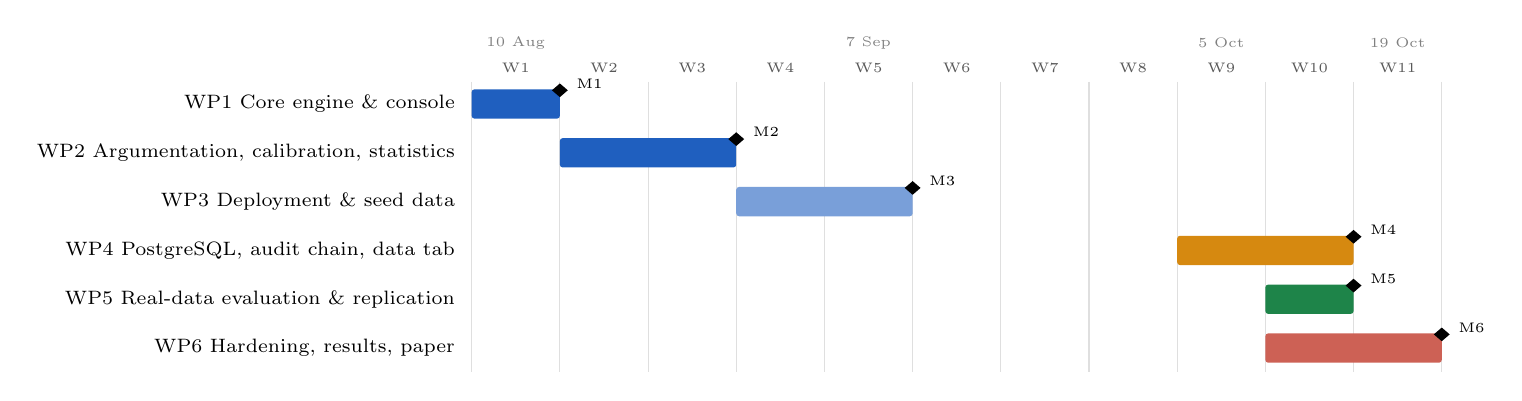
\begin{tikzpicture}[font=\scriptsize, x=1.12cm, y=0.62cm]
% grid
\foreach \w in {1,...,11} {
  \draw[gray!25] (\w,0.45) -- (\w,-5.5);
  \node[font=\tiny, gray!70!black] at (\w+0.5,0.75) {W\w};
}
\draw[gray!25] (12,0.45) -- (12,-5.5);
\node[font=\tiny, gray] at (1.5,1.25) {10 Aug}; \node[font=\tiny, gray] at (5.5,1.25) {7 Sep}; \node[font=\tiny, gray] at (9.5,1.25) {5 Oct}; \node[font=\tiny, gray] at (11.5,1.25) {19 Oct};
% tasks
\def\ganttbar#1#2#3#4#5{%
  \node[anchor=east, font=\scriptsize] at (0.92,#1) {#2};
  \fill[#5, rounded corners=1pt] (#3,#1-0.3) rectangle (#4,#1+0.3);
}
\ganttbar{0}{WP1 Core engine \& console}{1}{2}{cM}
\ganttbar{-1}{WP2 Argumentation, calibration, statistics}{2}{4}{cM}
\ganttbar{-2}{WP3 Deployment \& seed data}{4}{6}{cM!60}
\ganttbar{-3}{WP4 PostgreSQL, audit chain, data tab}{9}{11}{cR}
\ganttbar{-4}{WP5 Real-data evaluation \& replication}{10}{11}{cG}
\ganttbar{-5}{WP6 Hardening, results, paper}{10}{12}{cP!80}
% milestones
\foreach \x/\y/\l in {2/0/M1, 4/-1/M2, 6/-2/M3, 11/-3/M4, 11/-4/M5, 12/-5/M6} {
  \fill[black] (\x,\y) ++(0,0.42) -- ++(0.09,-0.14) -- ++(-0.09,-0.14) -- ++(-0.09,0.14) -- cycle;
  \node[font=\tiny, anchor=west] at (\x+0.08,\y+0.42) {\l};
}
\end{tikzpicture}
\caption{Project schedule (11 weeks, 10 August to 25 October 2026) derived from the commit history; diamonds mark milestones M1--M6 (Table~\ref{tab:milestones}). Weeks 6--8 contain no commits.}
\label{fig:gantt}
\end{figure*}

\subsubsection{Milestones and Verification Gates}
Each milestone was accepted against a verification gate expressed as passing tests or a generated result (Table~\ref{tab:milestones}).

\begin{table}[!t]
\centering
\caption{Milestones and Verification Gates}
\label{tab:milestones}
\scriptsize
\setlength{\tabcolsep}{2.5pt}
\begin{tabular}{@{}p{0.45cm}p{1.9cm}p{0.95cm}p{4.0cm}@{}}
\toprule
ID & Milestone & Date & Verification gate \\
\midrule
M1 & Protocol prototype & 15--16 Aug & Contract Net places patients; live console streams every step; same seed gives same result \\
M2 & Deliberation layer & 27 Aug & Grounded labelling passes textbook cases (reinstatement, even cycle); honest hospitals never overruled \\
M3 & Deployable system & 3--9 Sep & Docker stack starts in one command; dashboard test count matches suite \\
M4 & Database of record & 13 Oct & App cannot change capacity; owner cannot change real data; edited or deleted audit row breaks the chain \\
M5 & Real-data evaluation & 13--14 Oct & Cold-start occupancy error below 5 pts; Phoenix replicates with unchanged code \\
M6 & Final results & 15--20 Oct & All results regenerated from JSON; risk-based checks reported as negative \\
\bottomrule
\end{tabular}
\end{table}

\subsubsection{Risk Management}
Table~\ref{tab:risks} lists the principal project risks and the mitigations that were actually implemented.

\begin{table}[!t]
\centering
\caption{Risk Identification and Mitigation Matrix}
\label{tab:risks}
\scriptsize
\setlength{\tabcolsep}{2.5pt}
\begin{tabular}{@{}p{0.4cm}p{2.2cm}p{0.85cm}p{3.75cm}@{}}
\toprule
ID & Risk & Severity & Implemented mitigation \\
\midrule
R1 & Results depend on simulated behaviour & High & Every behavioural parameter swept; truthful-but-cautious control arm; ranges reported \\
R2 & Simulated hospitals unlike real ones & High & Per-pool Erlang-B fit to HHS data; cold-start validation; untuned second city \\
R3 & Non-reproducible runs & High & SHA-256-seeded random streams; fresh-process reproducibility test (two defects found and fixed) \\
R4 & Truthful hospitals wrongly penalised & Critical & Two-predicate attestation; spot checks restricted to capacity claims; safety tests \\
R5 & Collusion defeats reactive checks & High & Uniform random spot checks; cartel experiments \\
R6 & Tampering with records & High & Trigger locks, column grants, hash-chained audit log, checkpoints \\
R7 & Deliberation cost grows with run length & Medium & Indexed ledger queries (5$\times$ faster audit, identical output) \\
\bottomrule
\end{tabular}
\end{table}

% =========================================================================
\section{Technical Specification}
\label{sec:spec}
% =========================================================================

\subsection{Functional Requirements}
The requirements are organised by pipeline stage. Each is implemented and covered by the test suite.

\textbf{Stage 1: Network and data ingestion (FR-1).}
FR-1.1: build each study network from the HHS facility reports \cite{hhs_capacity_dataset} for a chosen week: staffed inpatient beds, occupied beds, staffed adult ICU beds and occupied ICU beds, keyed by CMS Certification Number (CCN).
FR-1.2: join capability (cardiac, neurological, trauma, obstetric, burns, catheterisation-room count) from the CMS Provider of Services file \cite{cms_pos} on CCN.
FR-1.3: load pairwise OSRM road times \cite{luxen2011osrm} and add a handover allowance.
FR-1.4: label every simulator input as observed, derived or assumed, and generate the provenance report from code.

\textbf{Stage 2: Agent assessment (FR-2).}
FR-2.1: each resource agent assesses a request from its own pool state and returns feasibility, preparation time, capability match $\kappa\in[0,1]$, post-acceptance strain and a private opportunity cost.
FR-2.2: a hospital's bidding policy decides what to report. The truthful assessment is retained privately for defence.
FR-2.3: the hospital's self-protection reserve is relaxed for acuity 3 and released entirely for acuity $\ge4$.

\textbf{Stage 3: Negotiation (FR-3).}
FR-3.1: announce an anonymised call for proposals (pseudonymous patient token, resource, specialty, acuity, deadline, expected stay) to the eight nearest peers by road time, and to sixteen in a second round.
FR-3.2: collect all bids in one parallel 2-minute window.
FR-3.3: reserve the winner's unit for 45\,min, and re-award to the runner-up if the reservation race is lost.
FR-3.4: retry failed requests every 20\,min while the deadline allows.

\textbf{Stage 4: Verification and deliberation (FR-4).}
FR-4.1: append every capacity refusal to the ledger before examining it.
FR-4.2: challenge a capability refusal that the public register contradicts.
FR-4.3: challenge a capacity refusal when the refuser accepted the same resource within 60\,min, or has a recent refusal-then-acceptance history.
FR-4.4: let the challenged hospital defend or sign, or have its refusal struck out by grounded labelling, and hold it to its truthful bid.
FR-4.5: spot-check a configurable fraction of uncontradicted capacity refusals.
FR-4.6: never compel a hospital beyond its real capacity.

\textbf{Stage 5: Award and fairness (FR-5).}
FR-5.1: discard bids that cannot meet the deadline before scoring.
FR-5.2: score surviving bids on time to care, capability, strain and fairness credit, collapsing towards speed for acuity $\ge4$.
FR-5.3: allow a burden objection only for acuity $\le3$ and only when a comparable alternative exists.
FR-5.4: attach a plain-English rationale to every award.

\textbf{Stage 6: Recording and audit (FR-6).}
FR-6.1: append each agreement, with the hash of its canonical terms, to a Merkle-linked ledger block.
FR-6.2: persist each negotiation (request, every agent decision, challenges, allocation, ledger block) in one database transaction.
FR-6.3: audit every insert, update and delete with before and after values and actor.
FR-6.4: provide chain verification and checkpointing.

\textbf{Stage 7: Monitoring and interaction (FR-7).}
FR-7.1: stream every protocol step to the console over WebSocket.
FR-7.2: let a reviewer edit occupancy and hospital behaviour, then restore the reported data.
FR-7.3: flag impossible or copied weekly reports (Data Integrity agent).
FR-7.4: report unmet needs and the fullest pools (Regional Monitor).

\subsection{Non-Functional Requirements}
Table~\ref{tab:nfr} lists the quantitative non-functional requirements and how each is verified.

\begin{table}[!t]
\centering
\caption{Quantitative Non-Functional Requirements and Verification}
\label{tab:nfr}
\scriptsize
\setlength{\tabcolsep}{2.2pt}
\begin{tabular}{@{}p{0.8cm}p{1.55cm}p{2.5cm}p{2.5cm}@{}}
\toprule
ID & Category & Requirement & Verification \\
\midrule
NFR-1 & Latency & p99 decision time $<1$\,s per transfer & \texttt{realtime.py} timing of every transfer \\
NFR-2 & Throughput & one bid window per round, independent of peer count & protocol design; message bus log \\
NFR-3 & Privacy & no occupancy value in any message; no global view & bus audit; leakage model; tests \\
NFR-4 & Safety & zero false accusations of truthful hospitals & cautious-hospital control arms; tests \\
NFR-5 & Integrity & real data immutable; any audit-row edit detected & database tests as owner and app role \\
NFR-6 & Atomicity & a negotiation is fully persisted or not at all & single-transaction write; smoke test \\
NFR-7 & Reproducibility & identical results for (scenario, seed) in any process & fresh-process test \\
NFR-8 & Realism & cold-start occupancy MAE $<5$\,pts & cold-start validation script \\
NFR-9 & Portability & core runs on the Python standard library & dependency-free install; CI-style test run \\
NFR-10 & Determinism & award never delegated to a language model & LLM off by default; ablation flag \\
\bottomrule
\end{tabular}
\end{table}

\subsection{Assumptions and Constraints}
\textbf{Assumptions.} (A1) Each hospital's capability (specialties, catheterisation rooms) is public and accurately listed in the CMS register. (A2) Agreements are recorded on a ledger that no single hospital can rewrite. (A3) Hospitals may misreport their own capacity but cannot forge other hospitals' ledger entries or the independent co-signature. (A4) Road time plus a fixed handover allowance is common knowledge.

\textbf{Constraints.} (C1) No message may contain a hospital's occupancy count. (C2) A patient may be assigned only to a hospital that can treat them, has a unit free above its reserve, and can begin care before the deadline. (C3) Fairness may reorder clinically comparable options but may never delay a critically ill patient. (C4) No decision may depend on a non-deterministic component; the language model, if enabled, only explains.

\subsection{Feasibility Study}
\subsubsection{Technical feasibility}
The protocol's computational load is small. A negotiation evaluates at most sixteen peers, builds an argumentation framework of a few dozen arguments, and computes its grounded labelling by fixed-point iteration in time polynomial in the number of arguments \cite{modgil2009algorithms}. Ed25519 signing and verification take about 0.43\,ms and 0.86\,ms per operation \cite{bernstein2012ed25519}. Ledger lookups are indexed by receiver, refuser and time. The measured median decision time is 3.55\,ms with ledger-backed challenge and 13.9\,ms in the adversarial setting (Section~\ref{sec:res-latency}), several orders of magnitude below the 90-minute shortest clinical window. A full 14-day simulation of 27 hospitals runs on a laptop.

\subsubsection{Data feasibility}
Every input that decides \emph{who can take a patient} is public. Beds, ICU beds and weekly occupancy come from HHS \cite{hhs_capacity_dataset}, capability and catheterisation rooms from CMS \cite{cms_pos}, roads from OpenStreetMap through OSRM \cite{luxen2011osrm}, and case-mix from California HCAI \cite{hcai_transfers}. All are public domain or openly licensed and are vendored in the repository, so the system runs offline. For Houston, 8 inputs are observed, 4 derived and 6 assumed (Table~\ref{tab:prov}).

\subsubsection{Economic and operational feasibility}
All software is open source: Python, FastAPI, PostgreSQL, pgAdmin and Docker. The system runs on commodity hardware with no licence or cloud cost. Operationally, \mahros{} reduces coordinator time per transfer from 50.3\,min (telephone search) to 1.1\,min (Section~\ref{sec:res-honest}). A deployment would integrate with each hospital's existing bed-management system instead of replacing it.

\subsubsection{Social, legal and ethical feasibility}
No patient-identifiable data are processed. Patients are referenced only by HMAC-SHA256 pseudonyms, and announcements carry clinical need but no demographic attributes. Hospitals never disclose occupancy, which removes the main commercial obstacle to regional data sharing. The accountability \mahros{} adds mirrors an obligation regulators already recognise for emergency patients \cite{emtala489}.

\subsection{System Specification}
\subsubsection{Hardware}
\mahros{} has no special hardware requirements. Table~\ref{tab:hw} gives the host on which the Docker deployment and live console were run for this paper.

\begin{table}[!t]
\centering
\caption{Development and Deployment Host}
\label{tab:hw}
\scriptsize
\setlength{\tabcolsep}{3pt}
\begin{tabular}{@{}p{2.0cm}p{5.6cm}@{}}
\toprule
Component & Specification \\
\midrule
Processor & Intel Core i5-13420H (8 cores, 12 threads) \\
Memory & 16 GB (15.6 GB usable) \\
Operating system & Windows 11; Docker Desktop with Linux containers \\
GPU & Not required \\
Network & Not required at run time (data vendored) \\
\bottomrule
\end{tabular}
\end{table}

\subsubsection{Software stack}
Table~\ref{tab:sw} lists the software stack, with versions read from the running deployment.

\begin{table}[!t]
\centering
\caption{Software Stack (Versions from the Running Deployment)}
\label{tab:sw}
\scriptsize
\setlength{\tabcolsep}{2.5pt}
\begin{tabular}{@{}p{1.85cm}p{1.95cm}p{3.7cm}@{}}
\toprule
Layer & Component & Version / configuration \\
\midrule
Runtime & CPython & 3.13.17 (\texttt{python:3.13-slim}); core uses stdlib only \\
Web API & FastAPI / Starlette & 0.162.0 / 1.9.0, served by Uvicorn 0.54.0 \\
Live channel & WebSocket & protocol events streamed per step \\
Database & PostgreSQL & 16.15 (\texttt{postgres:16-alpine}) \\
DB driver & psycopg & 3.3.6 (binary) \\
Signatures & cryptography & 50.0.2, Ed25519; HMAC-SHA256 fallback \\
Admin UI & pgAdmin 4 & 8.14 \\
Orchestration & Docker / Compose & 29.3.1 / v5.1.1, three services \\
Analysis & stdlib statistics & paired $t$, TOST, Holm, bootstrap \\
Testing & pytest & 205 test functions; DB tests with live Postgres \\
Optional & Ollama / hosted LLM & explanations only; off by default \\
\bottomrule
\end{tabular}
\end{table}

% =========================================================================
\section{Design Approach and Details}
\label{sec:design}
% =========================================================================

\subsection{System Architecture}
Figure~\ref{fig:arch} shows the layered architecture. Real public data are calibrated into a network of hospital agents. A transfer manager per request runs the negotiation, a Verifier checks refusals against the public register and the transfer ledger, and every agreement, refusal and agent decision is persisted in PostgreSQL behind a hash-chained audit log. The same engine runs in the batch simulator and in the live console.

\begin{figure*}[!t]
\centering
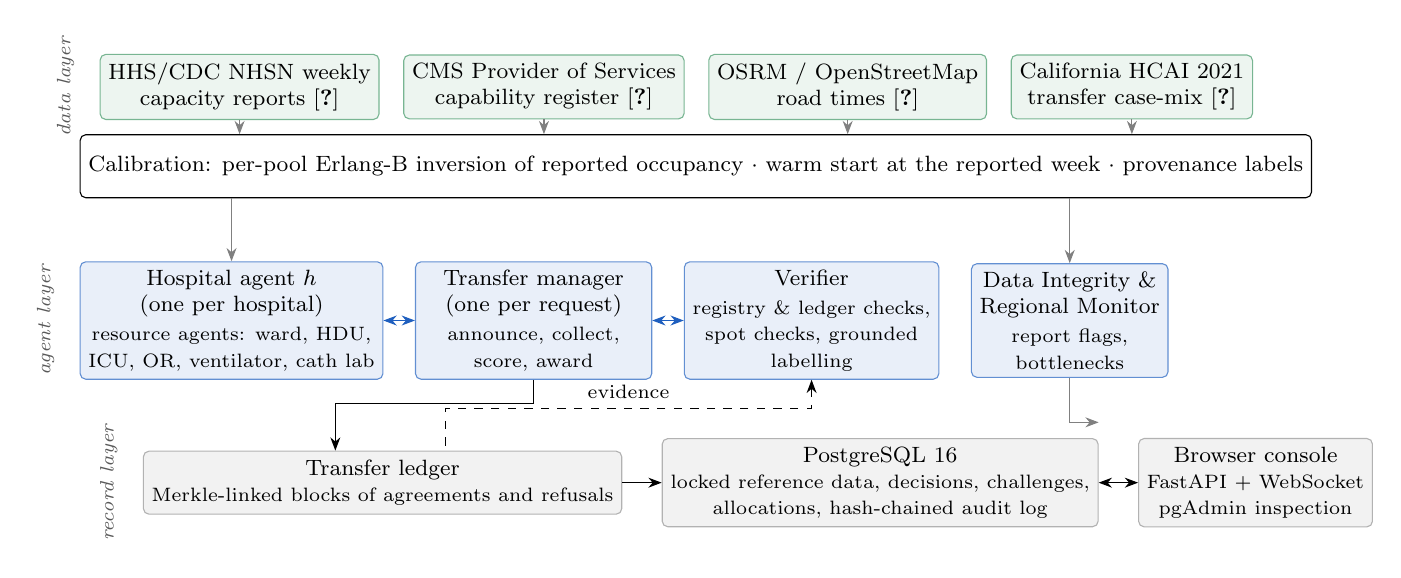
\begin{tikzpicture}[font=\footnotesize, >=Stealth,
  bx/.style={draw, rounded corners=2pt, align=center, inner sep=3pt, minimum height=8mm},
  agent/.style={bx, fill=cM!10, draw=cM!70},
  data/.style={bx, fill=cG!8, draw=cG!60},
  st/.style={bx, fill=gray!10, draw=gray!60},
  lab/.style={font=\scriptsize\itshape, text=gray!70!black},
]
\node[data, minimum width=3.0cm] (hhs) at (0,0) {HHS/CDC NHSN weekly\\capacity reports \cite{hhs_capacity_dataset}};
\node[data, minimum width=3.0cm, right=3mm of hhs] (cms) {CMS Provider of Services\\capability register \cite{cms_pos}};
\node[data, minimum width=3.0cm, right=3mm of cms] (osrm) {OSRM / OpenStreetMap\\road times \cite{luxen2011osrm}};
\node[data, minimum width=3.0cm, right=3mm of osrm] (hcai) {California HCAI 2021\\transfer case-mix \cite{hcai_transfers}};
\node[lab, left=2mm of hhs, rotate=90, anchor=south] {data layer};
\node[bx, fill=white, minimum width=12.9cm, below=6mm of $(cms)!0.5!(osrm)$] (cal) {Calibration: per-pool Erlang-B inversion of reported occupancy $\cdot$ warm start at the reported week $\cdot$ provenance labels};
\foreach \n in {hhs,cms,osrm,hcai} \draw[->, gray] (\n.south) -- (\n.south |- cal.north);
\node[agent, minimum width=3.3cm, below=8mm of cal.south west, anchor=north west] (ha) {Hospital agent $h$\\(one per hospital)\\[1pt]\scriptsize resource agents: ward, HDU,\\\scriptsize ICU, OR, ventilator, cath lab};
\node[agent, minimum width=3.0cm, right=4mm of ha] (tm) {Transfer manager\\(one per request)\\[1pt]\scriptsize announce, collect,\\\scriptsize score, award};
\node[agent, minimum width=3.0cm, right=4mm of tm] (ver) {Verifier\\[1pt]\scriptsize registry \& ledger checks,\\\scriptsize spot checks, grounded\\\scriptsize labelling};
\node[agent, minimum width=2.4cm, right=4mm of ver] (dia) {Data Integrity \&\\Regional Monitor\\[1pt]\scriptsize report flags,\\\scriptsize bottlenecks};
\node[lab, left=2mm of ha, rotate=90, anchor=south] {agent layer};
\draw[<->, cM] (ha) -- (tm);
\draw[<->, cM] (tm) -- (ver);
\draw[->, gray] (cal.south -| ha.north) -- (ha.north);
\draw[->, gray] (cal.south -| dia.north) -- (dia.north);
\node[st, minimum width=4.2cm, below=9mm of $(ha.south)!0.5!(tm.south)$] (led) {Transfer ledger\\\scriptsize Merkle-linked blocks of agreements and refusals};
\node[st, minimum width=4.2cm, right=5mm of led] (pg) {PostgreSQL 16\\\scriptsize locked reference data, decisions, challenges,\\\scriptsize allocations, hash-chained audit log};
\node[st, minimum width=2.9cm, right=5mm of pg] (ui) {Browser console\\\scriptsize FastAPI + WebSocket\\\scriptsize pgAdmin inspection};
\draw[->] (tm.south) -- ++(0,-3mm) -| ([xshift=-6mm]led.north);
\draw[<-, dashed] (ver.south) -- ++(0,-3.6mm) -| ([xshift=8mm]led.north) node[pos=0.25, above, font=\scriptsize]{evidence};
\draw[->] (led.east) -- (pg.west);
\draw[<->] (pg.east) -- (ui.west);
\draw[->, gray] (dia.south) |- ([yshift=2mm]pg.north east);
\node[lab, left=2mm of led, rotate=90, anchor=south] {record layer};
\end{tikzpicture}
\caption{System architecture of \mahros{}: data layer (real public sources), agent layer (hospital, transfer-manager, verifier, data-integrity and regional-monitor agents) and record layer (ledger, PostgreSQL, console).}
\label{fig:arch}
\end{figure*}

\subsection{Mathematical Formulation of the Pipeline}
\label{sec:pipeline}
Each transfer request $q$ is processed by a sequence of deterministic transformations, one per protocol phase.
\begin{enumerate}
\setlength{\itemsep}{2pt}
\item \emph{Announcement.} The origin selects the peer set by public road time only:
\begin{equation}
  P_q^{(k)} = \operatorname{arg\,min}^{(8k)}_{h\in\mathcal{H}\setminus\{o_q\}} \tau_{o_q,h},\qquad k\in\{1,2\},
  \label{eq:peers}
\end{equation}
the $8k$ nearest hospitals in round $k$, and sends each the public view $\pi(q)$, which carries no patient identity and no demographic data.
\item \emph{Private assessment and report.} Each peer computes a truthful assessment $A_h(q)=\mathrm{Assess}_h(\pi(q),x_h)$ and reports $\hat{A}_h(q)=\beta_h(A_h(q),q)$ through its bidding policy $\beta_h$. Only $\hat{A}_h$ leaves the hospital.
\item \emph{Verification.} For each refusal the Verifier computes a challenge set from public evidence only, namely the capability register $\mathcal{G}$ and the ledger $L$:
\begin{equation}
  C_q = \{\mathrm{ch}(h) : \hat{A}_h(q)=\textsc{ref} \wedge \mathrm{Contra}(h,q,\mathcal{G},L,t)\},
  \label{eq:challenges}
\end{equation}
where \textsc{ref} denotes a refusal.
\item \emph{Deliberation.} Bids, refusals, challenges and defences form an argumentation framework $\mathcal{AF}_q$, whose grounded labelling $\lambda_q=\mathrm{Grd}(\mathcal{AF}_q)$ strikes out undefended refusals. Each struck-out refusal is replaced by the hospital's truthful bid.
\item \emph{Award.} Among the surviving feasible bids $F_q=\{h:T_q(h)\le d_q\}$, the winner is
\begin{equation}
  h_q^\star=\operatorname*{arg\,max}_{h\in F_q}\;\bigl(S_h,\,-T_q(h),\,-\mathrm{id}(h)\bigr)\ \text{(lexicographic)},
  \label{eq:award}
\end{equation}
where $S_h$ is the score of Eq.~\eqref{eq:score}.
\item \emph{Record.} The agreement and every capacity refusal are appended to the ledger, $L\leftarrow L\,\Vert\,\langle q,h_q^\star,\mathrm{H}(\text{terms})\rangle$, and persisted atomically with the audit chain of Eq.~\eqref{eq:audit}.
\end{enumerate}

\subsection{Data and Calibration Layer}
\label{sec:data}
\emph{Study networks.} The headline network contains the 27 short-term acute hospitals with at least 25 inpatient beds within 40\,km of the Texas Medical Center in Houston: 8,176 inpatient beds and 1,029 staffed adult ICU beds in the reference week of 10 January 2021. Two multi-site system aggregates reporting hundreds of beds at administrative addresses are excluded, with stated reasons. The replication network contains 30 hospitals in metropolitan Phoenix, selected by the same code. Scenarios are real weeks chosen by observed occupancy (Table~\ref{tab:weeks}). Houston ran fuller in December 2023 than during the COVID-19 waves.

Table~\ref{tab:networks} summarises both networks by tier in their reference week.

\begin{table}[!t]
\centering
\caption{Study Networks by Tier, Reference Week 10 January 2021 (Reported Data)}
\label{tab:networks}
\scriptsize
\setlength{\tabcolsep}{2.2pt}
\begin{tabular}{@{}llccccc@{}}
\toprule
Region & Tier & Hosp. & Inpatient beds & ICU beds & Cath lab & Mean occ. \\
\midrule
\multirow{3}{*}{Houston} & 1 (community) & 10 & 675 & 114 & 8 & 0.83 \\
 & 2 (district) & 11 & 2,890 & 260 & 10 & 0.93 \\
 & 3 (tertiary) & 6 & 4,611 & 656 & 6 & 0.81 \\
\midrule
\multirow{3}{*}{Phoenix} & 1 (community) & 11 & 896 & 119 & 5 & 0.56 \\
 & 2 (district) & 8 & 2,356 & 382 & 6 & 0.82 \\
 & 3 (tertiary) & 11 & 6,220 & 959 & 8 & 0.77 \\
\bottomrule
\end{tabular}
\end{table}

\emph{Erlang-B calibration.} Each ward, HDU and ICU pool is modelled as an Erlang loss system with $c$ beds and offered load $a$ \cite{debruin2010erlang,green2002beds}. The blocking probability follows the stable recursion
\begin{equation}
  B(k,a)=\frac{a\,B(k-1,a)}{k + a\,B(k-1,a)},\quad k=1,\dots,c,\quad B(0,a)=1,
  \label{eq:erlang}
\end{equation}
and for the reported occupancy $\rho_h$ the offered load is obtained by bisection on
\begin{equation}
  a_{h,r}\bigl(1-B(c_{h,r},a_{h,r})\bigr) = \min(\rho_h,\bar\rho)\,c_{h,r},\qquad \bar\rho=0.95.
  \label{eq:inversion}
\end{equation}
By Little's law \cite{little1961proof}, the pool's arrival rate is $\lambda_{h,r}=a_{h,r}/\bar W_r$, using the realised lognormal mean stay ($\sigma=0.6$), scaled to a network mean of 4.6 days. The fit is per pool rather than aggregate, so an ICU-heavy facility does not overflow its ward. The cap $\bar\rho$ exists because a stationary loss system cannot sit at 100\% occupancy; facilities above the cap are fitted to it and keep their reported value for validation.

\emph{Warm start and escalation.} Runs start at the occupancy reported that week. Patients already present receive a length-biased remaining stay: for a lognormal$(\mu,\sigma)$ stay, the length-biased stay is lognormal$(\mu+\sigma^2,\sigma)$, and the time left is a uniform fraction of it. Each admission escalates with probability 0.14 after a lognormal delay (mean 7\,h), which gives transfer requests for about 4.5\% of admissions, consistent with the U.S.\ critical-care transfer share \cite{iwashyna2009networks}. The resource each request needs follows the case-mix of 37,439 real California transfers (Table~\ref{tab:casemix}).

\emph{Provenance.} Table~\ref{tab:prov} lists every simulator input with its provenance class.

\begin{table}[!t]
\centering
\caption{Provenance of Simulator Inputs (Houston): 8 Observed, 4 Derived, 6 Assumed}
\label{tab:prov}
\scriptsize
\setlength{\tabcolsep}{2.5pt}
\begin{tabular}{@{}p{2.2cm}p{1.0cm}p{4.3cm}@{}}
\toprule
Input & Class & Source or rule \\
\midrule
Specialty capability & observed & CMS POS Q1 2021 certification codes \\
Catheterisation labs & observed & CMS POS catheterisation room count \\
ICU beds & observed & HHS staffed adult ICU beds (7-day avg.) \\
Paediatric capability & observed & HHS staffed paediatric ICU beds $>0$ \\
Identifier, name, coordinates & observed & HHS CCN, name, geocoded address \\
Travel time & observed & OSRM over OpenStreetMap \\
\midrule
Ward beds & derived & inpatient beds minus ICU and HDU \\
Admission mix & derived & observed bed composition / pool stay \\
Arrival rate & derived & Erlang-B inversion, Eq.~\eqref{eq:inversion} \\
Tier & derived & beds vs.\ national percentiles, gated on ICU \\
\midrule
HDU beds; ventilators & assumed & $0.5\times$ and $0.8\times$ ICU beds \\
OR slots; coordinators & assumed & 1 per 30 and 1 per 150 inpatient beds \\
Handover; mean stay & assumed & 12\,min (swept 8--20); 4.6 days (cited) \\
\bottomrule
\end{tabular}
\end{table}

\begin{table}[!t]
\centering
\caption{Escalation Case-Mix from 37,439 California Transfers (2021)}
\label{tab:casemix}
\scriptsize
\begin{tabular}{@{}lr|lr@{}}
\toprule
Profile & Share & Profile & Share \\
\midrule
HDU, general        & 19.7\% & ICU, neuro          & 9.1\% \\
ICU, general        & 18.2\% & OR, general         & 5.7\% \\
Ventilator          & 15.1\% & HDU, obstetric      & 3.5\% \\
Cath lab, cardiac   & 12.5\% & OR, trauma          & 2.5\% \\
ICU, cardiac        & 12.5\% & ICU, paediatric     & 1.1\% \\
                    &        & ICU, burns          & 0.1\% \\
\bottomrule
\end{tabular}
\end{table}

\subsection{Agent Layer}
\label{sec:agents}
\emph{Resource agents.} One agent per pool assesses a request. It refuses with \texttt{resource\_not\_offered} if the pool has zero capacity, with \texttt{no\_specialty\_capability} if the capability match is $\kappa=0$, and with \texttt{at\_self\_protection\_reserve} if the free units do not exceed the reserve. The match $\kappa$ is 1 for a listed specialty, 0.9 for general care and 0.6 for an unlisted specialty at a tertiary centre. The reserve is one ICU unit and two ward units, falls by one for acuity 3, and is zero for acuity $\ge4$. Otherwise the agent reports preparation time, $\kappa$, and the post-acceptance strain
\begin{equation}
  \sigma^{+}_{h,r}(q) = \frac{x_{h,r}+y_{h,r}+1}{c_{h,r}},
  \label{eq:strain}
\end{equation}
where $y_{h,r}$ counts reservations. It also computes a private opportunity cost $\pi_h(q)=(\sigma^{+})^3(1+0.25\,\ell_q/1440)$, which never leaves the hospital.

\emph{Hospital agents and behaviour policies.} A bidding policy maps the truthful assessment to the reported one. \textsc{Honest} reports the truth. \textsc{Protective} fabricates a refusal with probability $\phi$ when the patient is expensive ($\ell_q\ge24$\,h) or the hospital would exceed a comfort threshold $\theta$ (default 0.55), never for acuity 5, and chooses the most plausible excuse. \textsc{Cautious} never lies but holds two extra units in reserve; it is the control against false accusations. \textsc{Colluding} is protective and also refuses whenever a fellow cartel member refused the same resource in the last 60\,min. Policies are assigned in nested, incentive-ordered fashion, starting from tertiary centres.

\subsection{Contract-Net Negotiation}
\label{sec:protocol}
Algorithm~\ref{alg:mahros} gives the negotiation. Its distinctive step is deliberation (lines 5--15) between bidding and award. All bids arrive in one parallel window, so a round costs 2\,min regardless of the number of peers; that parallelism is what replaces the serial telephone search.

\begin{algorithm}[!t]
\caption{\mahros{} negotiation for request $q$ at time $t$}
\label{alg:mahros}
\small
\begin{algorithmic}[1]
\Require request $q$, hospitals $\mathcal{H}$, ledger $L$, register $\mathcal{G}$
\Ensure agreement or failure
\For{$k=1,2$}
  \State $P \gets$ the $8k$ peers nearest to $o_q$ (Eq.~\ref{eq:peers})
  \State send CFP$(\pi(q))$ to $P$; $B\gets\{\hat{A}_p(q)\}_{p\in P}$
  \State $\mathcal{A}\gets$ bid and refusal arguments for $B$
  \State $L.\textsc{AppendRefusal}(b)$ for every capacity refusal $b$
  \ForAll{refusals $b\in B$}
    \If{attested, capacity reason, $U<\theta_{\text{spot}}$}
      \State spot check: \textsc{Attest}$(b)$ or challenge
    \ElsIf{$\textsc{Contra}(b,\mathcal{G},L,t)$}
      \State challenge; defence if \textsc{Defend}$(b)$ (or \textsc{Attest})
    \EndIf
  \EndFor
  \State add admissible burden objections
  \State $\lambda\gets\textsc{Grounded}(\mathcal{A})$
  \State replace each \textsc{out} refusal by its truthful bid
  \State $t\gets t+0.75$; rank on-time bids by Eq.~\eqref{eq:score}
  \For{candidate $h$ in rank order}
    \If{$h.\textsc{Reserve}(q, t+45)$} \State $L.\textsc{AppendAgreement}(q,h)$; \Return agreement \EndIf
  \EndFor
  \If{$t+2 \ge d_q$} \textbf{break} \EndIf
\EndFor
\State \Return failure
\end{algorithmic}
\end{algorithm}

\subsection{Refusal Verification}
\label{sec:verify}
The design principle is that \emph{capability is public and capacity is private}. A capability refusal is checked against the public register. Reason \texttt{no\_specialty\_capability} is contradicted if $s_q\in\mathcal{G}_h$, and \texttt{resource\_not\_offered} if $h$ is listed as operating pool $r_q$ with positive capacity. A capacity refusal is checked against the refuser's own recorded commitments, the only public evidence that bears on it. It is directly contradicted if
\begin{equation}
  \exists\, e\in L:\; e.\text{receiver}=h,\; e.\text{resource}=r_q,\; t-60\le e.t\le t ,
  \label{eq:direct}
\end{equation}
that is, if the hospital accepted a patient needing the same resource within the hour. Otherwise it is challenged on history if, within the last 240\,min, the hospital made a recorded capacity refusal followed within 60\,min by its own acceptance of the same resource. Every capacity refusal is appended to the ledger \emph{before} examination, so it becomes evidence against later ones. The check achieves accountability without disclosure: it never reads a hospital's state, only what the hospital publicly committed to.

\subsection{Dispute Resolution by Grounded Semantics}
\label{sec:argumentation}
Each negotiation builds a Dung framework $\mathcal{AF}=(\mathcal{A},\rightarrow)$ \cite{dung1995acceptability} with exactly four attack rules. A challenge attacks the refusal it names. A defence or attestation attacks the challenge it answers. A burden objection attacks the objector's own bid. A counter-offer attacks the hospital's original bid. Hospitals never attack one another directly. The labelling $\lambda:\mathcal{A}\to\{\textsc{in},\textsc{out},\textsc{undec}\}$ is the least fixed point of
\begin{align}
  \lambda(A)=\textsc{in} \;&\Leftarrow\; \forall B\rightarrow A:\ \lambda(B)=\textsc{out}, \label{eq:in}\\
  \lambda(A)=\textsc{out} \;&\Leftarrow\; \exists B\rightarrow A:\ \lambda(B)=\textsc{in}, \label{eq:out}
\end{align}
which yields the unique grounded extension \cite{baroni2011semantics}. Figure~\ref{fig:af} shows the two patterns that arise: reinstatement \cite{caminada2006reinstatement} when the hospital defends, and defeat when it cannot. A struck-out refusal is replaced by the hospital's truthful bid. If that bid is still infeasible, the refusal stands, so no hospital is ever compelled beyond its real capacity. Because an honest refusal is backed by the refuser's real state, it can always be defended, and truthful hospitals are never overruled.

\begin{figure}[!t]
\centering
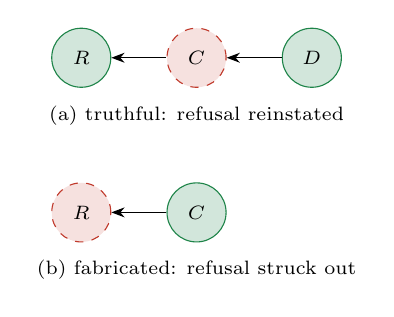
\begin{tikzpicture}[font=\scriptsize, >=Stealth, node distance=7mm,
  arg/.style={draw, circle, minimum size=7.5mm, inner sep=0pt, align=center},
  inn/.style={arg, fill=cG!20, draw=cG}, outt/.style={arg, fill=cP!15, draw=cP, dashed}]
\node[inn] (r1) {$R$};
\node[outt, right=of r1] (c1) {$C$};
\node[inn, right=of c1] (d1) {$D$};
\draw[->] (c1) -- (r1); \draw[->] (d1) -- (c1);
\node[below=1mm of c1, align=center] {(a) truthful: refusal reinstated};
\node[outt, below=12mm of r1] (r2) {$R$};
\node[inn, right=of r2] (c2) {$C$};
\draw[->] (c2) -- (r2);
\node[below=1mm of c2, align=center] {(b) fabricated: refusal struck out};
\end{tikzpicture}
\caption{Grounded labelling of a challenged refusal. $R$ refusal, $C$ evidence-backed challenge, $D$ defence or signed attestation. Green: \textsc{in}; red dashed: \textsc{out}.}
\label{fig:af}
\end{figure}

\subsection{Signed Refusals (Attestation)}
\label{sec:attest}
In the attested protocol a challenged hospital discharges the challenge only by signing the contested predicate. It may sign \textsc{no\_unit\_available} (no unit was free for this request at time $t$) or \textsc{at\_declared\_reserve} (the only free units lie inside a declared reserve). The second predicate lets a cautious hospital certify its true position. The canonical payload (hospital, request, resource, predicate, time, nonce) is signed with the hospital's Ed25519 key \cite{bernstein2012ed25519} and co-signed by an independent key, such as a regulator or record-system vendor, so a cartel cannot vouch for itself. No bed count is ever signed. A protective hospital that fabricated a refusal declines to sign with probability $\delta$, the deterrence, and otherwise signs falsely. Post hoc, a signed ``no unit available'' followed within 5\,min by the same hospital's acceptance of that resource generates an advisory \emph{audit referral} for a regulator.

\subsection{Collusion Defence}
\label{sec:collusion}
A cartel whose members never accept a resource while any member's refusal of it is outstanding leaves no contradiction for Eq.~\eqref{eq:direct} to find. \mahros{} therefore adds two mechanisms. The first is \emph{co-refusal monitoring}, which tracks the temporal follow-on lift
\begin{equation}
  \mathrm{FL}(a,b) = \frac{\Pr[b \text{ refuses } r \mid a \text{ refused } r \text{ within } 60\,\text{min}]}{\Pr[b \text{ refuses}]}
  \label{eq:lift}
\end{equation}
as an advisory signal \cite{porter1993bidrigging}. The second is \emph{random spot checks}: with probability $\theta_{\text{spot}}$ a capacity refusal that nothing contradicts is challenged anyway and must be signed. This is random inspection \cite{becker1968crime} in protocol form. A risk-based variant checks hospitals already caught at a higher rate $\theta'$.

\subsection{Award Scoring and Fairness}
\label{sec:scoring}
Bids that cannot meet the deadline are discarded, never traded off. For each surviving bid the time term blends relative speed with the absolute safety margin:
\begin{equation}
  \tau^{\star}_h = 0.6\Bigl(1-\tfrac{T_h - T_{\min}}{T_{\max}-T_{\min}}\Bigr) + 0.4\,\mathrm{clip}_{[0,1]}\!\Bigl(\tfrac{d_q - T_h}{d_q - t_q}\Bigr).
  \label{eq:timeterm}
\end{equation}
The score is
\begin{equation}
  S_h = 0.45\,\tau^{\star}_h + 0.25\,\kappa_h + 0.15\,(1-\sigma^{+}_h) - 0.15\,\gamma_h,
  \label{eq:score}
\end{equation}
and for acuity $\ge4$ it collapses to $S'_h=0.75\,(0.45\tau^{\star}_h+0.25\kappa_h)/0.70+0.25\,S_h$, so equity never costs a critically ill patient time. The fairness credit is the relative deviation of a hospital's recent acceptances from its capacity share over the last 200 acceptances:
\begin{equation}
  \gamma_h = \mathrm{clip}_{[-1,1]}\!\left(\frac{n_h/n - \sigma_h}{\sigma_h}\right).
  \label{eq:credit}
\end{equation}
A hospital with $\gamma_h>0.35$ may object to its own bid, but only for acuity $\le3$ and only when another bid is within 15\,min of its own time to care.

\subsection{Ledger and Database Integrity}
\label{sec:db}
Agreements and capacity refusals form a ledger of Merkle-linked blocks of 16 entries \cite{merkle1988signature,haber1991timestamp}. Each block header commits to the previous block's hash and the Merkle root of its entries, and each agreement carries the SHA-256 hash of its canonical terms. Per-receiver, per-refuser and time-window indices keep every challenge lookup sub-linear. In PostgreSQL, real reference data (hospitals, capabilities, weekly reports, travel times) have no application write grant and are locked by a \texttt{BEFORE} trigger, even against the owner. Live state (occupancy, behaviour policy) is editable only through column grants and a capacity \texttt{CHECK}. Records are append-only. Every change fires a trigger that appends to a hash-chained audit log under an advisory lock:
\begin{equation}
\begin{aligned}
  h_i &= \mathrm{SHA256}(m_i),\\
  m_i &= h_{i-1}\,\|\,\mathit{ts}_i\,\|\,\mathit{actor}_i\,\|\,\mathit{op}_i\,\|\,\mathit{table}_i\\
      &\qquad \|\,\mathit{pk}_i\,\|\,\mathit{before}_i\,\|\,\mathit{after}_i,
\end{aligned}
  \label{eq:audit}
\end{equation}
with $h_0=0^{64}$. A verification function recomputes the chain and reports the first broken row, which catches any edited, inserted or deleted audit row, together with any checkpoint that no longer matches. A checkpoint exported outside the database also detects a wholesale rewrite by a superuser.

\subsection{Request Lifecycle}
Figure~\ref{fig:states} gives the state machine of a transfer request as implemented.

\begin{figure}[!t]
\centering
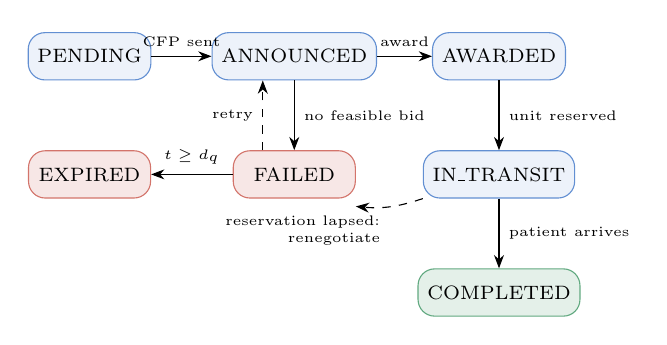
\begin{tikzpicture}[font=\scriptsize, >=Stealth, node distance=5mm and 6mm,
  s/.style={draw=cM!70, fill=cM!8, rounded corners=6pt, minimum width=1.55cm, minimum height=6mm, align=center},
  t/.style={s, fill=cG!12, draw=cG!70}, f/.style={s, fill=cP!12, draw=cP!70}]
\node[s] (pend) at (0,0) {PENDING};
\node[s] (ann) at (2.6,0) {ANNOUNCED};
\node[s] (awd) at (5.2,0) {AWARDED};
\node[f] (exp) at (0,-1.5) {EXPIRED};
\node[f] (fail) at (2.6,-1.5) {FAILED};
\node[s] (tr) at (5.2,-1.5) {IN\_TRANSIT};
\node[t] (done) at (5.2,-3.0) {COMPLETED};
\draw[->] (pend) -- node[above, font=\tiny]{CFP sent} (ann);
\draw[->] (ann) -- node[above, font=\tiny]{award} (awd);
\draw[->] (awd) -- node[right, font=\tiny]{unit reserved} (tr);
\draw[->] (tr) -- node[right, font=\tiny]{patient arrives} (done);
\draw[->] (ann) -- node[right, font=\tiny]{no feasible bid} (fail);
\draw[->] (fail) -- node[above, font=\tiny]{$t\ge d_q$} (exp);
\draw[->, dashed] ([xshift=-4mm]fail.north) -- node[left, font=\tiny]{retry} ([xshift=-4mm]ann.south);
\draw[->, dashed] (tr.south west) to[bend left=12] node[below left, font=\tiny, align=right]{reservation lapsed:\\renegotiate} ([yshift=-1mm]fail.south east);
\end{tikzpicture}
\caption{Transfer-request state machine. A request completes only if care starts before its deadline $d_q$; otherwise it expires.}
\label{fig:states}
\end{figure}

% =========================================================================
\section{Design Models and Diagrams}
\label{sec:models}
% =========================================================================

\subsection{Data Flow Diagrams}
\subsubsection{Level 0 (context)}
Figure~\ref{fig:dfd0} shows \mahros{} as a single process exchanging data with its four external entities.

\begin{figure}[!t]
\centering
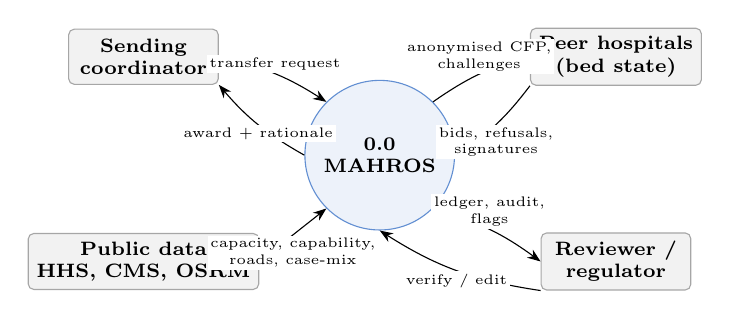
\begin{tikzpicture}[font=\scriptsize, >=Stealth]
\node[proc, circle, minimum size=1.9cm, font=\scriptsize\bfseries] (sys) at (0,0) {0.0\\\mahros{}};
\node[ext, minimum width=1.9cm, minimum height=7mm] (coord) at (-3.0,1.25) {Sending\\coordinator};
\node[ext, minimum width=1.9cm, minimum height=7mm] (hosp) at (3.0,1.25) {Peer hospitals\\(bed state)};
\node[ext, minimum width=1.9cm, minimum height=7mm] (data) at (-3.0,-1.35) {Public data\\HHS, CMS, OSRM};
\node[ext, minimum width=1.9cm, minimum height=7mm] (rev) at (3.0,-1.35) {Reviewer /\\regulator};
\draw[flow] (coord.east) to[bend left=10] node[flowlab, above]{transfer request} (sys.north west);
\draw[flow] (sys.west) to[bend left=10] node[flowlab, below]{award + rationale} (coord.south east);
\draw[flow] (sys.north east) to[bend left=10] node[flowlab, above]{anonymised CFP,\\challenges} (hosp.west);
\draw[flow] (hosp.south west) to[bend left=10] node[flowlab, below]{bids, refusals,\\signatures} (sys.east);
\draw[flow] (data.east) -- node[flowlab, below]{capacity, capability,\\roads, case-mix} (sys.south west);
\draw[flow] (sys.south east) to[bend left=10] node[flowlab, above]{ledger, audit,\\flags} (rev.west);
\draw[flow] (rev.south west) to[bend left=12] node[flowlab, below]{verify / edit} (sys.south);
\end{tikzpicture}
\caption{Level 0 data flow diagram (context level).}
\label{fig:dfd0}
\end{figure}

\subsubsection{Level 1 (subsystem decomposition)}
Figure~\ref{fig:dfd1} decomposes the system into seven processes and four data stores. Hospital private state (D4) is read only by process 3.0, running inside each hospital's own agent.

\begin{figure*}[!t]
\centering
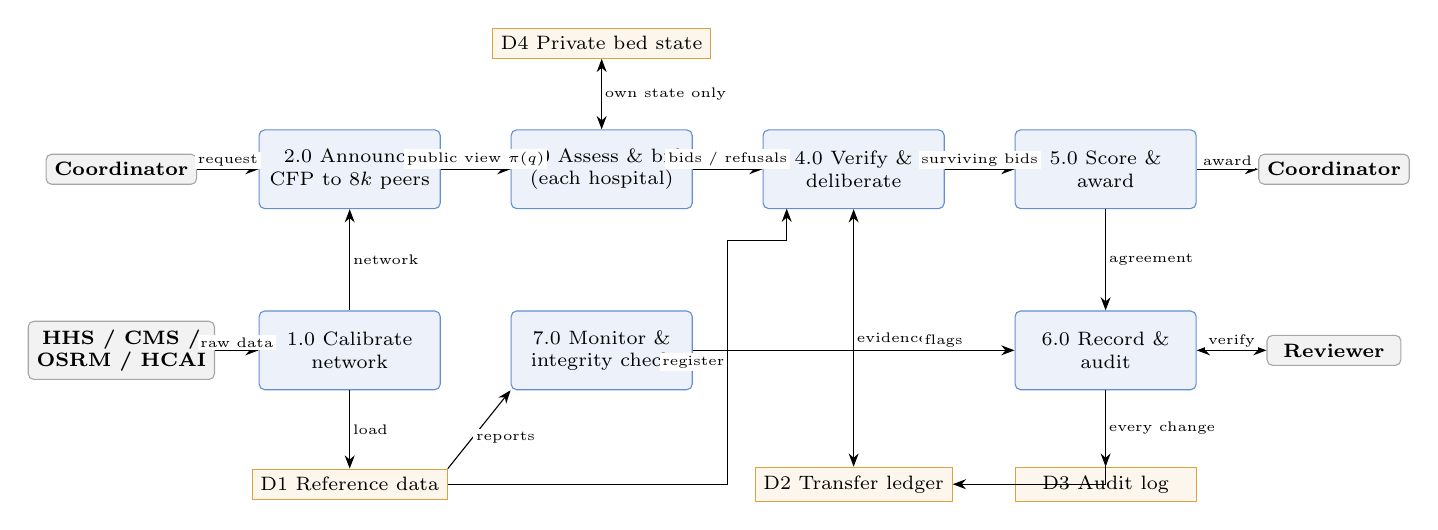
\begin{tikzpicture}[font=\scriptsize, >=Stealth]
\tikzset{p/.style={proc, minimum width=2.3cm, minimum height=1.0cm}}
\node[ext, minimum width=1.7cm] (coord) at (0,0) {Coordinator};
\node[p] (p2) at (2.9,0) {2.0 Announce\\CFP to $8k$ peers};
\node[p] (p3) at (6.1,0) {3.0 Assess \& bid\\(each hospital)};
\node[p] (p4) at (9.3,0) {4.0 Verify \&\\deliberate};
\node[p] (p5) at (12.5,0) {5.0 Score \&\\award};
\node[ext, minimum width=1.7cm] (coord2) at (15.4,0) {Coordinator};
\node[p] (p1) at (2.9,-2.3) {1.0 Calibrate\\network};
\node[p] (p6) at (12.5,-2.3) {6.0 Record \&\\audit};
\node[p] (p7) at (6.1,-2.3) {7.0 Monitor \&\\integrity check};
\node[ext, minimum width=1.7cm] (src) at (0,-2.3) {HHS / CMS /\\OSRM / HCAI};
\node[ext, minimum width=1.7cm] (rev) at (15.4,-2.3) {Reviewer};
\node[store, minimum width=2.3cm] (d1) at (2.9,-4.0) {D1 Reference data};
\node[store, minimum width=2.3cm] (d4) at (6.1,1.6) {D4 Private bed state};
\node[store, minimum width=2.3cm] (d2) at (9.3,-4.0) {D2 Transfer ledger};
\node[store, minimum width=2.3cm] (d3) at (12.5,-4.0) {D3 Audit log};
\draw[flow] (coord) -- node[flowlab, above]{request} (p2);
\draw[flow] (p2) -- node[flowlab, above]{public view $\pi(q)$} (p3);
\draw[flow] (p3) -- node[flowlab, above]{bids / refusals} (p4);
\draw[flow] (p4) -- node[flowlab, above]{surviving bids} (p5);
\draw[flow] (p5) -- node[flowlab, above]{award} (coord2);
\draw[flow, <->] (d4) -- node[flowlab, right]{own state only} (p3);
\draw[flow] (src) -- node[flowlab, above]{raw data} (p1);
\draw[flow] (p1) -- node[flowlab, right]{load} (d1);
\draw[flow] (d1.east) -- (7.7,-4.0) -- node[flowlab, pos=0.5, left]{register} (7.7,-0.9) -- (8.45,-0.9) -- (8.45,-0.5);
\draw[flow] (p1) -- node[flowlab, right]{network} (p2);
\draw[flow, <->] (p4) -- node[flowlab, right]{evidence} (d2);
\draw[flow] (p5) -- node[flowlab, right]{agreement} (p6);
\draw[flow] (p6) |- (d2.east);
\draw[flow] (p6) -- node[flowlab, right]{every change} (d3);
\draw[flow] (d1.north east) -- node[flowlab, right, pos=0.4]{reports} (p7.south west);
\draw[flow] (p7) -- node[flowlab, above, pos=0.78]{flags} (p6);
\draw[flow, <->] (rev) -- node[flowlab, above]{verify} (p6);
\end{tikzpicture}
\caption{Level 1 data flow diagram. D4 is held separately by every hospital agent and never leaves it; all other processes see only public data, bids and the ledger.}
\label{fig:dfd1}
\end{figure*}

\subsubsection{Level 2 (process 4.0, verify and deliberate)}
Figure~\ref{fig:dfd2} unpacks the deliberation process, the core of the verification mechanism.

\begin{figure*}[!t]
\centering
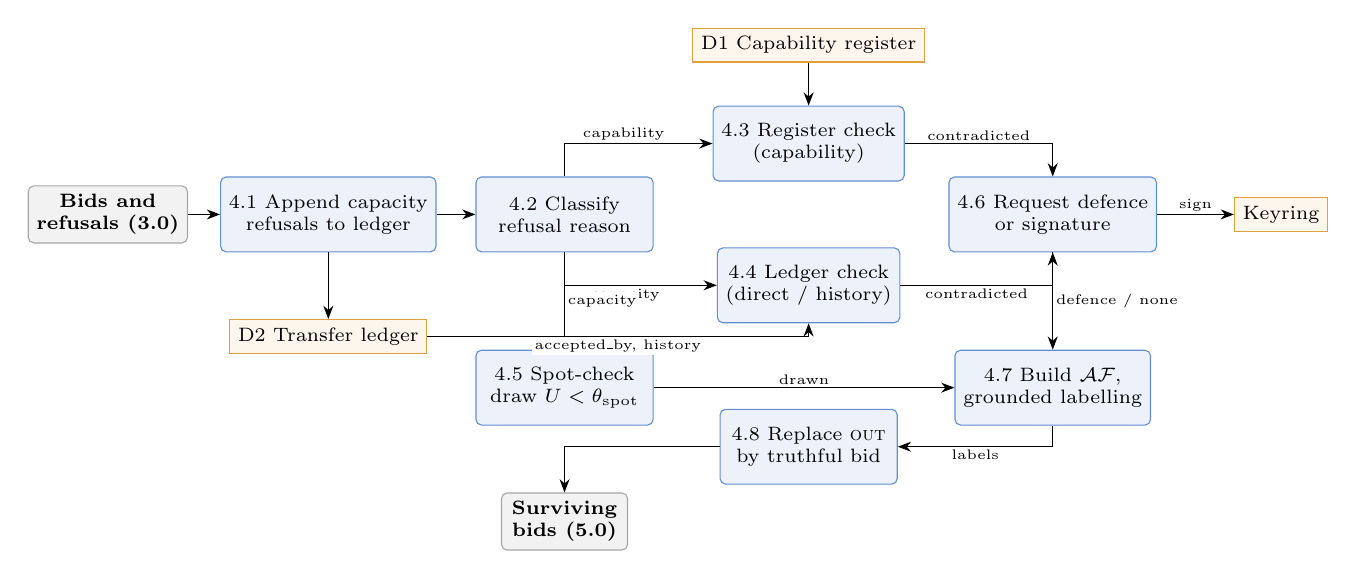
\begin{tikzpicture}[font=\scriptsize, >=Stealth]
\tikzset{p/.style={proc, minimum width=2.25cm, minimum height=0.95cm}}
\node[ext, minimum width=1.6cm] (in) at (0,0) {Bids and\\refusals (3.0)};
\node[p] (a) at (2.8,0) {4.1 Append capacity\\refusals to ledger};
\node[p] (b) at (5.8,0) {4.2 Classify\\refusal reason};
\node[p] (c) at (8.9,0.9) {4.3 Register check\\(capability)};
\node[p] (d) at (8.9,-0.9) {4.4 Ledger check\\(direct / history)};
\node[p] (e) at (5.8,-2.2) {4.5 Spot-check\\draw $U<\theta_{\text{spot}}$};
\node[p] (f) at (12.0,0) {4.6 Request defence\\or signature};
\node[p] (g) at (12.0,-2.2) {4.7 Build $\mathcal{AF}$,\\grounded labelling};
\node[p] (h) at (8.9,-2.95) {4.8 Replace \textsc{out}\\by truthful bid};
\node[ext, minimum width=1.6cm] (out) at (5.8,-3.9) {Surviving\\bids (5.0)};
\node[store] (reg) at (8.9,2.15) {D1 Capability register};
\node[store] (led) at (2.8,-1.55) {D2 Transfer ledger};
\node[store] (keys) at (14.9,0) {Keyring};
\draw[flow] (in) -- (a);
\draw[flow] (a) -- (b);
\draw[flow] (a) -- (led);
\draw[flow] (b) |- node[flowlab, pos=0.7, above]{capability} (c);
\draw[flow] (b) |- node[flowlab, pos=0.7, below]{capacity} (d);
\draw[flow] (b) -- node[flowlab, right]{capacity} (e);
\draw[flow] (reg) -- (c);
\draw[flow] (led) -| node[flowlab, pos=0.25, below]{accepted\_by, history} (d);
\draw[flow] (c) -| node[flowlab, pos=0.25, above]{contradicted} (f);
\draw[flow] (d) -| node[flowlab, pos=0.25, below]{contradicted} (f);
\draw[flow] (e) -- node[flowlab, above]{drawn} (g.west |- e);
\draw[flow] (f) -- node[flowlab, above]{sign} (keys);
\draw[flow] (f) -- node[flowlab, right]{defence / none} (g);
\draw[flow] (g) |- node[flowlab, pos=0.75, below]{labels} (h);
\draw[flow] (h) -| (out);
\end{tikzpicture}
\caption{Level 2 data flow diagram for process 4.0. Capability claims are checked against the register, capacity claims against the ledger; only contradicted or spot-checked refusals reach the defence step, and grounded labelling decides.}
\label{fig:dfd2}
\end{figure*}

\subsection{Use-Case Model}
Figure~\ref{fig:usecase} gives the use-case diagram. Three use cases are specified below.

\begin{figure}[!t]
\centering
\begin{tikzpicture}[font=\scriptsize, >=Stealth,
  uc/.style={draw=cM!70, fill=cM!6, ellipse, minimum width=2.75cm, minimum height=5.5mm, inner sep=1pt, align=center, font=\tiny}]
\newcommand{\stick}[3]{% x, y, label
  \draw[thick] (#1,#2+0.42) circle (0.09);
  \draw[thick] (#1,#2+0.33) -- (#1,#2+0.05) (#1-0.16,#2+0.24) -- (#1+0.16,#2+0.24)
               (#1,#2+0.05) -- (#1-0.12,#2-0.15) (#1,#2+0.05) -- (#1+0.12,#2-0.15);
  \node[font=\tiny, align=center, below] at (#1,#2-0.15) {#3};}
\draw[gray!70, rounded corners] (-1.55,-5.0) rectangle (1.55,1.15);
\node[font=\tiny\bfseries, gray!70!black] at (0,0.93) {MAHROS};
\node[uc] (u1) at (0,0.4) {UC1 Request transfer};
\node[uc] (u2) at (0,-0.4) {UC2 Bid on request};
\node[uc] (u3) at (0,-1.2) {UC3 Challenge refusal};
\node[uc] (u4) at (0,-2.0) {UC4 Defend / sign refusal};
\node[uc] (u5) at (0,-2.8) {UC5 Award and reserve};
\node[uc] (u6) at (0,-3.6) {UC6 Verify ledger \& audit};
\node[uc] (u7) at (0,-4.4) {UC7 Edit occupancy / policy};
\stick{-2.85}{0.0}{Sending\\coordinator}
\stick{-2.85}{-2.6}{Hospital\\agent}
\stick{2.85}{-1.4}{Verifier\\agent}
\stick{2.85}{-4.0}{Reviewer /\\regulator}
\draw (-2.65,0.2) -- (u1.west); \draw (-2.65,0.2) -- (u5.west);
\draw (-2.65,-2.4) -- (u2.west); \draw (-2.65,-2.4) -- (u4.west);
\draw (2.65,-1.2) -- (u3.east); \draw (2.65,-1.2) -- (u5.east);
\draw (2.65,-3.8) -- (u6.east); \draw (2.65,-3.8) -- (u7.east);
\draw[dashed, ->] (u3) -- node[right, font=\tiny]{\guillemotleft include\guillemotright} (u4);
\end{tikzpicture}
\caption{Use-case diagram of \mahros{}.}
\label{fig:usecase}
\end{figure}

\emph{UC1: Request transfer.}
Actor: sending coordinator. Pre-condition: the patient is admitted and needs a resource unavailable locally.
Main flow: (1) the coordinator selects resource, specialty and acuity; (2) the transfer manager pseudonymises the patient and announces a CFP to the eight nearest peers; (3) bids are collected in one window; (4) deliberation and award run (UC3--UC5); (5) the coordinator receives the receiving hospital, expected time to care and rationale.
Post-condition: the agreement is on the ledger and the request, decisions and allocation are in PostgreSQL.
Alternative flow: if no feasible bid survives and time remains, a second round asks sixteen peers; otherwise the request is retried every 20\,min until its deadline.

\emph{UC3/UC4: Challenge and defend a refusal.}
Actors: Verifier, hospital agent. Trigger: a refusal is contradicted by the register or the ledger, or is spot-checked.
Main flow: (1) the Verifier adds a challenge citing the ledger entries or register line; (2) the hospital defends or, in the attested protocol, signs the contested predicate; (3) grounded labelling reinstates the refusal.
Alternative flow: if the hospital cannot defend or declines to sign, the refusal is struck out and the hospital is held to its truthful bid. If that bid is also infeasible, the refusal stands.

\emph{UC2: Bid on a request.}
Actor: hospital agent. Trigger: a CFP arrives.
Main flow: (1) the resource agent for the requested pool assesses the anonymised request against the hospital's own state; (2) the bidding policy decides what to report; (3) the agent replies \textsc{propose} with time to care, capability match and strain, or \textsc{refuse} with a reason code, within the bid window.
Post-condition: the truthful assessment is retained privately for any later challenge; nothing about occupancy leaves the hospital.

\emph{UC5: Award and reserve.}
Actor: transfer manager. Pre-condition: deliberation is complete.
Main flow: (1) bids that cannot meet the deadline are discarded; (2) the rest are scored by Eq.~\eqref{eq:score}; (3) the winner's unit is reserved for 45\,min; (4) the agreement and its terms hash are appended to the ledger; (5) the other bidders receive \textsc{reject-proposal}.
Alternative flow: if the reservation race is lost to a concurrent award, the runner-up is tried.

\emph{UC6: Verify ledger and audit.}
Actor: reviewer or regulator. Main flow: (1) the reviewer requests verification; (2) the system recomputes every ledger block hash and Merkle root and every audit-row hash, and compares checkpoints; (3) it reports either an intact chain or the first broken row and the reason (link broken, contents changed, checkpoint mismatch).

\emph{UC7: Edit occupancy or policy.}
Actor: reviewer. Main flow: (1) the reviewer edits a pool's occupancy or a hospital's behaviour policy in the Hospital-data tab; (2) the API validates the value, and the database's \texttt{CHECK} constraint independently keeps occupancy within capacity; (3) the update trigger appends an audit row with before and after values and the actor; (4) the next negotiation reads the new state.
Alternative flow: an attempt to change capacity or reference data is rejected by trigger, even for the database owner.

\subsection{Class Model}
Figure~\ref{fig:classes} shows the principal classes of the implementation, with their key attributes and operations.

\begin{figure*}[!t]
\centering
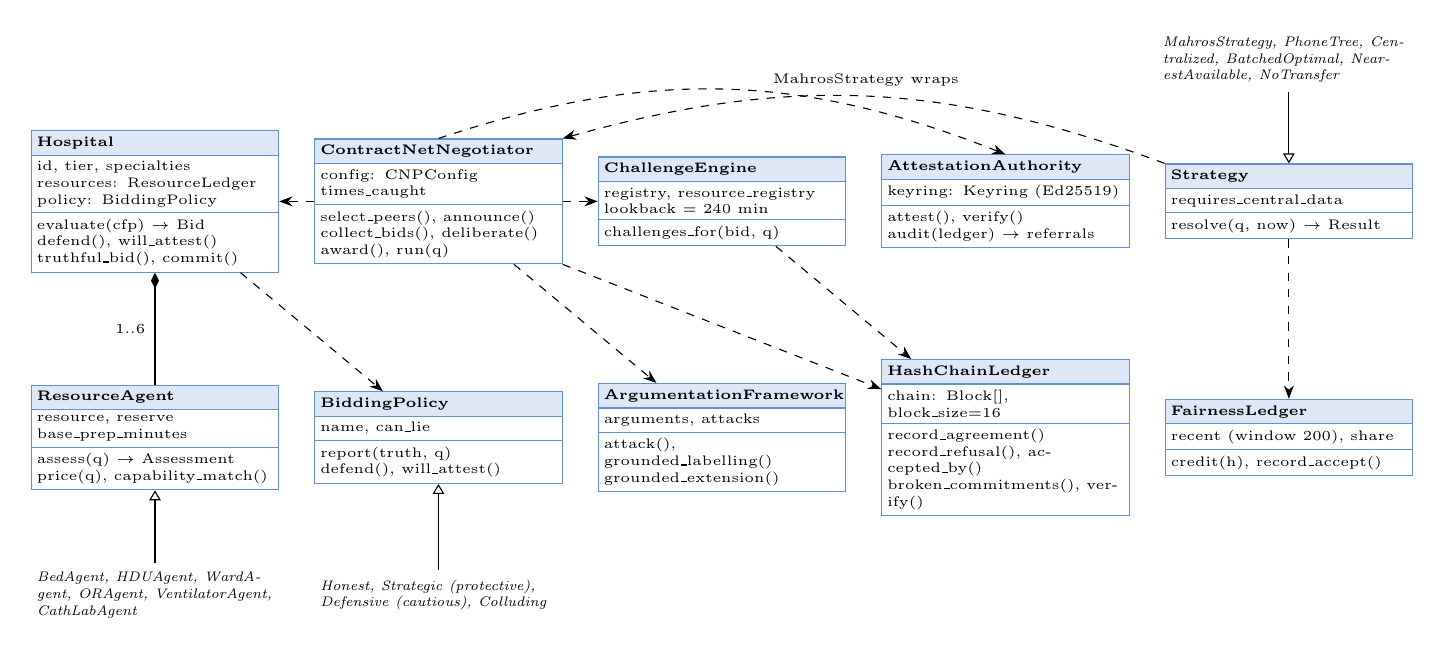
\begin{tikzpicture}[font=\tiny, >=Stealth,
  cls/.style={draw=cM!70, rectangle split, rectangle split parts=3, rectangle split part fill={cM!15,white,white}, text width=3.0cm, inner sep=2pt, align=left, font=\tiny},
  inh/.style={-{Triangle[open]}, thin}, comp/.style={-{Diamond[]}, thin}, uses/.style={->, dashed, thin}]
\node[cls] (hosp) at (0,0) {\textbf{Hospital}
  \nodepart{second} id, tier, specialties\\ resources: ResourceLedger\\ policy: BiddingPolicy
  \nodepart{third} evaluate(cfp) $\to$ Bid\\ defend(), will\_attest()\\ truthful\_bid(), commit()};
\node[cls] (ra) at (0,-3.0) {\textbf{ResourceAgent}
  \nodepart{second} resource, reserve\\ base\_prep\_minutes
  \nodepart{third} assess(q) $\to$ Assessment\\ price(q), capability\_match()};
\node[cls] (pol) at (3.6,-3.0) {\textbf{BiddingPolicy}
  \nodepart{second} name, can\_lie
  \nodepart{third} report(truth, q)\\ defend(), will\_attest()};
\node[cls] (cnp) at (3.6,0) {\textbf{ContractNetNegotiator}
  \nodepart{second} config: CNPConfig\\ times\_caught
  \nodepart{third} select\_peers(), announce()\\ collect\_bids(), deliberate()\\ award(), run(q)};
\node[cls] (ch) at (7.2,0) {\textbf{ChallengeEngine}
  \nodepart{second} registry, resource\_registry\\ lookback = 240 min
  \nodepart{third} challenges\_for(bid, q)};
\node[cls] (af) at (7.2,-3.0) {\textbf{ArgumentationFramework}
  \nodepart{second} arguments, attacks
  \nodepart{third} attack(), grounded\_labelling()\\ grounded\_extension()};
\node[cls] (att) at (10.8,0) {\textbf{AttestationAuthority}
  \nodepart{second} keyring: Keyring (Ed25519)
  \nodepart{third} attest(), verify()\\ audit(ledger) $\to$ referrals};
\node[cls] (led) at (10.8,-3.0) {\textbf{HashChainLedger}
  \nodepart{second} chain: Block[], block\_size=16
  \nodepart{third} record\_agreement()\\ record\_refusal(), accepted\_by()\\ broken\_commitments(), verify()};
\node[cls] (str) at (14.4,0) {\textbf{Strategy}
  \nodepart{second} requires\_central\_data
  \nodepart{third} resolve(q, now) $\to$ Result};
\node[cls] (fair) at (14.4,-3.0) {\textbf{FairnessLedger}
  \nodepart{second} recent (window 200), share
  \nodepart{third} credit(h), record\_accept()};
\node[font=\tiny, align=left, text width=3.0cm] (sub1) at (0,-5.0) {\textit{BedAgent, HDUAgent, WardAgent, ORAgent, VentilatorAgent, CathLabAgent}};
\node[font=\tiny, align=left, text width=3.0cm] (sub2) at (3.6,-5.0) {\textit{Honest, Strategic (protective), Defensive (cautious), Colluding}};
\node[font=\tiny, align=left, text width=3.0cm] (sub3) at (14.4,-4.85) {};
\node[font=\tiny, align=left, text width=3.2cm] (sub4) at (14.4,1.8) {\textit{MahrosStrategy, PhoneTree, Centralized, BatchedOptimal, NearestAvailable, NoTransfer}};
\draw[comp] (ra) -- node[left]{1..6} (hosp);
\draw[uses] (hosp) -- (pol);
\draw[uses] (cnp) -- (hosp.east);
\draw[uses] (cnp) -- (ch);
\draw[uses] (cnp) -- (af);
\draw[uses] (cnp.north) to[bend left=20] (att.north);
\draw[uses] (ch) -- (led);
\draw[uses] (cnp.south east) -- (led);
\draw[uses] (str) -- (fair);
\draw[uses] (str.north west) to[bend right=18] node[above]{MahrosStrategy wraps} (cnp.north east);
\draw[inh] (sub1) -- (ra);
\draw[inh] (sub2) -- (pol);
\draw[inh] (sub4) -- (str);
\end{tikzpicture}
\caption{Class diagram of the core engine (names as in the source code). Solid diamond: composition; dashed: uses; open triangle: specialisation.}
\label{fig:classes}
\end{figure*}

\subsection{Sequence Diagrams}
Figure~\ref{fig:seq1} traces one negotiation in which a protective hospital's false capacity refusal is challenged and struck out. Figure~\ref{fig:seq2} traces the same transfer requested from the console and persisted to PostgreSQL.

\begin{figure*}[!t]
\centering
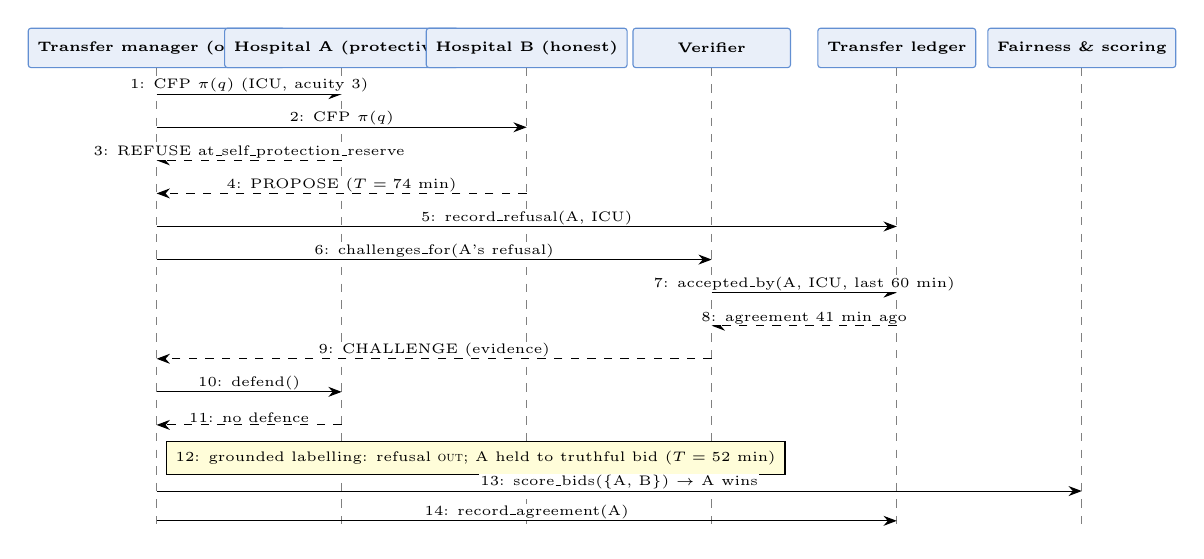
\begin{tikzpicture}[font=\tiny, >=Stealth, x=2.35cm, y=0.42cm]
\foreach \i/\n in {0/Transfer manager (origin), 1/Hospital A (protective), 2/Hospital B (honest), 3/Verifier, 4/Transfer ledger, 5/Fairness \& scoring} {
  \node[draw=cM!70, fill=cM!10, rounded corners=1pt, minimum width=2.0cm, minimum height=5mm, font=\tiny\bfseries, align=center] at (\i,0) {\n};
  \draw[dashed, gray] (\i,-0.6) -- (\i,-14.6);
}
\def\msg#1#2#3#4{\draw[->] (#1,#3) -- node[above, font=\tiny, fill=white, inner sep=0.5pt]{#4} (#2,#3);}
\def\ret#1#2#3#4{\draw[->, dashed] (#1,#3) -- node[above, font=\tiny, fill=white, inner sep=0.5pt]{#4} (#2,#3);}
\msg{0}{1}{-1.4}{1: CFP $\pi(q)$ (ICU, acuity 3)}
\msg{0}{2}{-2.4}{2: CFP $\pi(q)$}
\ret{1}{0}{-3.4}{3: REFUSE at\_self\_protection\_reserve}
\ret{2}{0}{-4.4}{4: PROPOSE ($T=74$ min)}
\msg{0}{4}{-5.4}{5: record\_refusal(A, ICU)}
\msg{0}{3}{-6.4}{6: challenges\_for(A's refusal)}
\msg{3}{4}{-7.4}{7: accepted\_by(A, ICU, last 60 min)}
\ret{4}{3}{-8.4}{8: agreement 41 min ago}
\ret{3}{0}{-9.4}{9: CHALLENGE (evidence)}
\msg{0}{1}{-10.4}{10: defend()}
\ret{1}{0}{-11.4}{11: no defence}
\node[draw, fill=yellow!15, font=\tiny, align=left, anchor=west] at (0.05,-12.4) {12: grounded labelling: refusal \textsc{out}; A held to truthful bid ($T=52$ min)};
\msg{0}{5}{-13.4}{13: score\_bids(\{A, B\}) $\to$ A wins}
\msg{0}{4}{-14.3}{14: record\_agreement(A)}
\end{tikzpicture}
\caption{Sequence of a negotiation with a challenged false refusal. Times are illustrative of the message order, not measured values.}
\label{fig:seq1}
\end{figure*}

\begin{figure*}[!t]
\centering
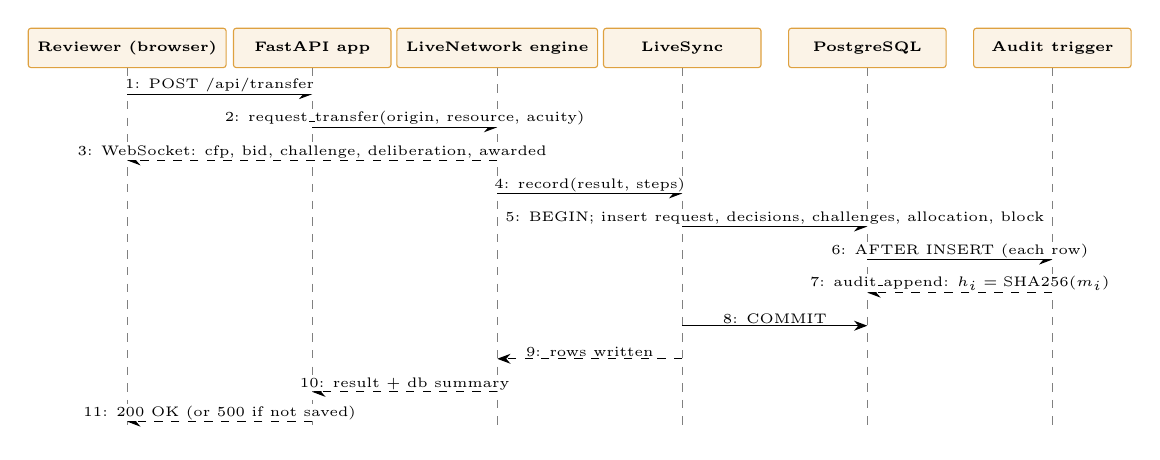
\begin{tikzpicture}[font=\tiny, >=Stealth, x=2.35cm, y=0.42cm]
\foreach \i/\n in {0/Reviewer (browser), 1/FastAPI app, 2/LiveNetwork engine, 3/LiveSync, 4/PostgreSQL, 5/Audit trigger} {
  \node[draw=cR!80, fill=cR!10, rounded corners=1pt, minimum width=2.0cm, minimum height=5mm, font=\tiny\bfseries, align=center] at (\i,0) {\n};
  \draw[dashed, gray] (\i,-0.6) -- (\i,-11.6);
}
\def\msg#1#2#3#4{\draw[->] (#1,#3) -- node[above, font=\tiny, fill=white, inner sep=0.5pt]{#4} (#2,#3);}
\def\ret#1#2#3#4{\draw[->, dashed] (#1,#3) -- node[above, font=\tiny, fill=white, inner sep=0.5pt]{#4} (#2,#3);}
\msg{0}{1}{-1.4}{1: POST /api/transfer}
\msg{1}{2}{-2.4}{2: request\_transfer(origin, resource, acuity)}
\ret{2}{0}{-3.4}{3: WebSocket: cfp, bid, challenge, deliberation, awarded}
\msg{2}{3}{-4.4}{4: record(result, steps)}
\msg{3}{4}{-5.4}{5: BEGIN; insert request, decisions, challenges, allocation, block}
\msg{4}{5}{-6.4}{6: AFTER INSERT (each row)}
\ret{5}{4}{-7.4}{7: audit\_append: $h_i=\mathrm{SHA256}(m_i)$}
\msg{3}{4}{-8.4}{8: COMMIT}
\ret{3}{2}{-9.4}{9: rows written}
\ret{2}{1}{-10.4}{10: result + db summary}
\ret{1}{0}{-11.3}{11: 200 OK (or 500 if not saved)}
\end{tikzpicture}
\caption{Sequence of a console transfer persisted to PostgreSQL. The whole negotiation is one transaction; a failed write is reported rather than silently dropped.}
\label{fig:seq2}
\end{figure*}

\subsection{User Interface}
Figure~\ref{fig:console} shows the live console. The \emph{Live negotiation} tab runs transfers on the real Houston network, optionally with protective hospitals, and animates the six protocol steps as they stream in. The \emph{Hospital data} tab edits occupancy and behaviour, each edit audited with before and after values and actor, and restores the reported data. The \emph{Results} tab shows the generated dashboard. pgAdmin is bundled so that every table can be inspected and tampering can be attempted directly.

\begin{figure*}[!t]
\centering
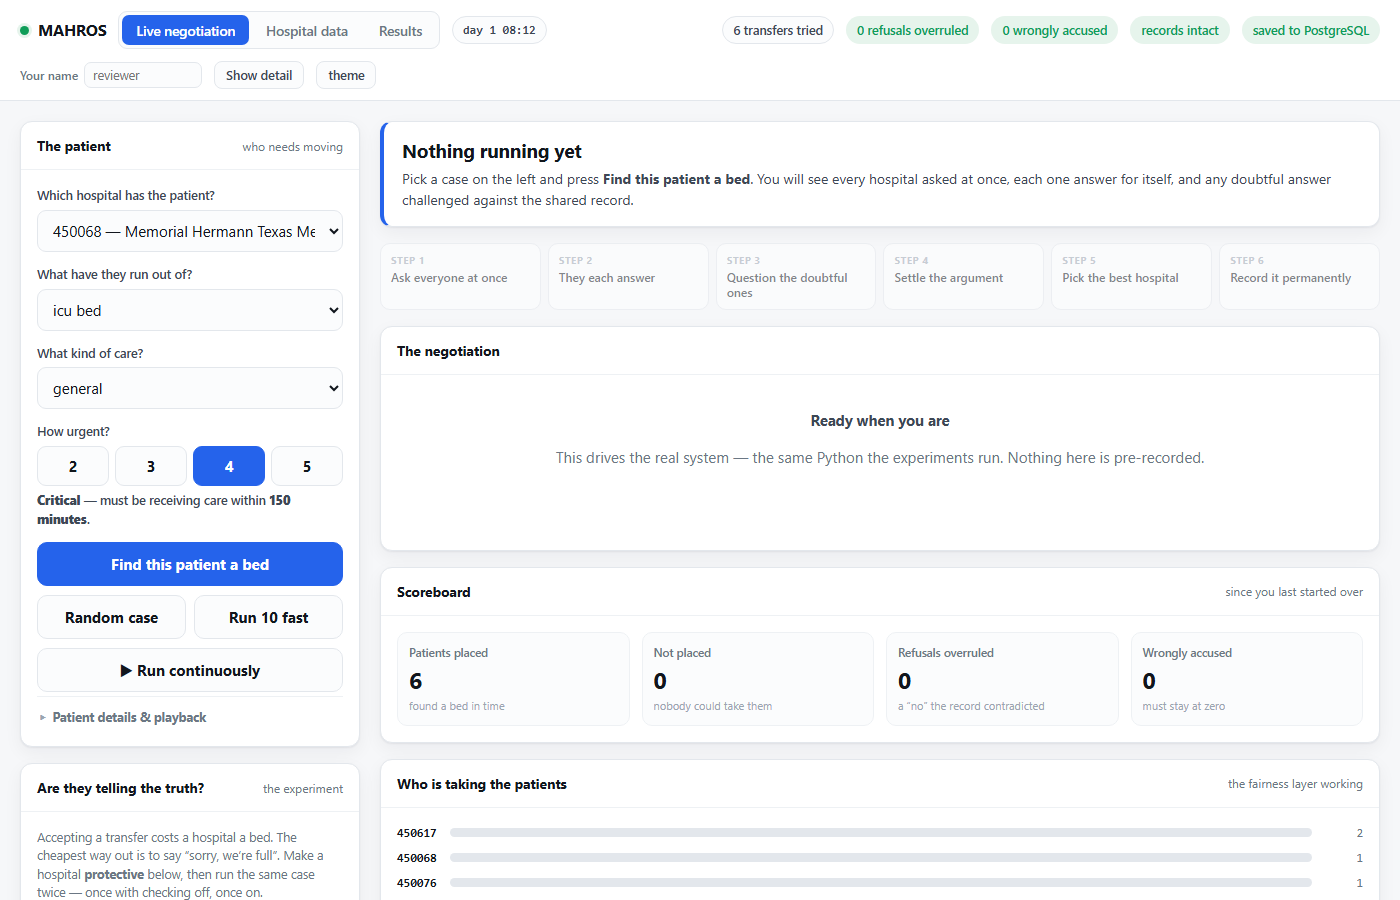
\includegraphics[width=0.78\textwidth]{figures/console.png}
\caption{The \mahros{} live console (Live negotiation tab) connected to PostgreSQL. Left: the case to place. Centre: the six protocol steps and a scoreboard of placements, overruled refusals and wrongly accused hospitals. Top right: record integrity and persistence status.}
\label{fig:console}
\end{figure*}

% =========================================================================
\section{Implementation}
\label{sec:implementation}
% =========================================================================

\subsection{Software Organisation}
The engine is a Python package whose modules correspond one-to-one to the layers of Fig.~\ref{fig:arch}:
\begin{itemize}
\setlength{\itemsep}{1pt}
\item \texttt{hospital/}: resource agents, hospital agent and behaviour policies.
\item \texttt{negotiation/}: Contract Net, challenge engine, argumentation, attestation, collusion, scoring and message bus.
\item \texttt{sim/}: real-network builder, warm start, scenarios, the five baselines, event loop and metrics.
\item \texttt{calibration/}: vendored HHS, CMS, OSRM and HCAI data with their loaders.
\item \texttt{ledger/}, \texttt{integrity/}, \texttt{fairness/}, \texttt{privacy/} and \texttt{eval/}: the hash-chained ledger, the Data Integrity rules, burden metrics, pseudonymisation and leakage model, and statistics with a Hungarian solver.
\item \texttt{db/}: PostgreSQL schema, store and live synchronisation.
\item \texttt{server/}: FastAPI application and the browser console.
\end{itemize}
The core uses only the Python standard library, so every experiment runs without building an environment. Each experiment is one script that writes a JSON result file. A build script regenerates the results document from those files, and the figures in this paper are drawn from data tables generated the same way, so no reported number is typed by hand.

\subsection{Simulation Engine}
The simulator is a discrete-event loop over a priority queue of timed events: admission, escalation, negotiation, care start, expiry, discharge and periodic sampling. Each run is fully determined by \texttt{(scenario, seed)}. All random streams, including hospital behaviour and spot-check selection, are seeded from SHA-256 digests rather than Python's per-process randomised \texttt{hash()}, and a regression test checks that a run reproduces exactly in a fresh process. Every strategy, MAHROS and baselines alike, implements one interface, \texttt{resolve(request, now)}, and runs in the same loop on the same patient stream, so differences in outcome come from the allocation logic alone.

\subsection{Message Bus and Decentralisation Audit}
All inter-agent traffic passes through a message bus that records FIPA-style performatives (\textsc{cfp}, \textsc{propose}, \textsc{refuse}, \textsc{accept-proposal}, \textsc{reject-proposal}) with sender, receiver and payload. Baselines log their traffic to the same bus, including every telephone answer, so all arms are audited on equal terms. The bus computes the decision concentration, the largest share of capacity-bearing messages received by any single node, and checks that no node obtains a global view.

Table~\ref{tab:messages} lists every message type and its exact payload. No field carries an occupancy count, a bed count or a patient identity.

\begin{table}[!t]
\centering
\caption{Protocol Messages and Payloads}
\label{tab:messages}
\scriptsize
\setlength{\tabcolsep}{2.5pt}
\begin{tabular}{@{}p{1.55cm}p{1.6cm}p{4.35cm}@{}}
\toprule
Performative & Direction & Payload fields \\
\midrule
\textsc{cfp} & origin $\to$ peer & request id, origin, pseudonymous patient token, resource, specialty, acuity, created / expires time, expected stay \\
\textsc{propose} & peer $\to$ origin & feasible, time to care, capability match \\
\textsc{refuse} & peer $\to$ origin & feasible = false, reason code \\
\textsc{accept-proposal} & origin $\to$ winner & time to care \\
\textsc{reject-proposal} & origin $\to$ others & none \\
challenge / defence & within $\mathcal{AF}$ & claim text, reason code, evidence (ledger ids) \\
attestation & peer $\to$ verifier & hospital, request, resource, predicate, time, nonce, two Ed25519 signatures \\
\bottomrule
\end{tabular}
\end{table}

\subsection{Privacy Measure}
\label{sec:privacy}
For a pool of capacity $c$, an observer's prior over occupancy is uniform on $\{0,\dots,c\}$. A message consistent with a subset $\mathcal{S}$ of occupancy levels discloses
\begin{equation}
  I = \log_2(c+1) - \log_2|\mathcal{S}|\ \text{bits}.
  \label{eq:bits}
\end{equation}
A \mahros{} offer rules out only the levels at or above the reserve, about 0.06 bits on a 26-bed ICU. A capacity refusal bounds occupancy to the top few levels, about 3.2 bits. A centralised message carrying strain reveals all $\log_2(c+1)$ bits. Attestation adds nothing, because the signed predicate is exactly what the refusal already asserted. Patients are referenced only by an HMAC-SHA256 pseudonym, and free-text notes pass through a pattern-based scrubber for names, record numbers, phone numbers, dates and e-mail addresses before anything leaves the origin.

\subsection{Data Integrity Rules}
\label{sec:integrity-rules}
The Data Integrity agent applies hand-checkable rules to every real weekly report. A report is \emph{red} (impossible as reported) if any of the following holds:
\begin{itemize}
\setlength{\itemsep}{0pt}
\item it shows more inpatients than staffed beds, more ICU patients than ICU beds, or more ICU beds than inpatient beds (with a 0.5 tolerance for 7-day averaging);
\item it reports zero inpatients in a staffed hospital that reports patients in other weeks;
\item its bed count is below half the median of the surrounding $\pm8$ weeks.
\end{itemize}
A report is \emph{amber} (looks copied or stale) if the same non-zero inpatient count appears four or more weeks running, or if occupancy jumps by at least 30 points for one week and returns to within 10 points. Flags are stored in the \texttt{report\_flags} table and shown per hospital in the console.

\subsection{Deployment Architecture}
Figure~\ref{fig:deploy} shows the Docker Compose deployment. On start, the application container initialises the schema idempotently, loads the vendored real data through the privileged loader role, and serves the console and API through an unprivileged application role.

\begin{figure}[!t]
\centering
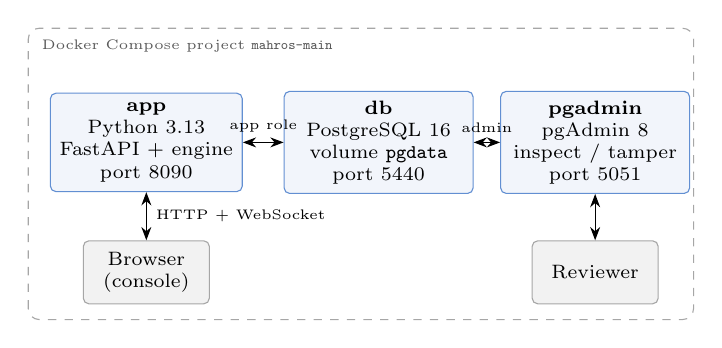
\begin{tikzpicture}[font=\scriptsize, >=Stealth,
  ctr/.style={draw=cM!70, fill=cM!6, rounded corners=2pt, align=center, minimum width=2.4cm, minimum height=1.25cm},
  usr/.style={draw=gray!70, fill=gray!10, rounded corners=2pt, align=center, minimum width=1.6cm, minimum height=0.8cm}]
\draw[dashed, gray!70, rounded corners] (-0.2,-2.75) rectangle (8.25,0.95);
\node[font=\tiny, gray!70!black, anchor=north west] at (-0.15,0.92) {Docker Compose project \texttt{mahros-main}};
\node[ctr] (app) at (1.3,-0.5) {\textbf{app}\\Python 3.13\\FastAPI + engine\\port 8090};
\node[ctr] (db) at (4.25,-0.5) {\textbf{db}\\PostgreSQL 16\\volume \texttt{pgdata}\\port 5440};
\node[ctr] (pga) at (7.0,-0.5) {\textbf{pgadmin}\\pgAdmin 8\\inspect / tamper\\port 5051};
\node[usr] (br) at (1.3,-2.15) {Browser\\(console)};
\node[usr] (rv) at (7.0,-2.15) {Reviewer};
\draw[<->] (app) -- node[above, font=\tiny]{app role} (db);
\draw[<->] (pga) -- node[above, font=\tiny]{admin} (db);
\draw[<->] (br) -- node[right, font=\tiny]{HTTP + WebSocket} (app);
\draw[<->] (rv) -- (pga);
\end{tikzpicture}
\caption{Deployment: three containers started by one \texttt{docker compose up}. Data persist in a named volume; \texttt{down -v} reloads the real data.}
\label{fig:deploy}
\end{figure}

\subsection{API Specification}
Table~\ref{tab:api} lists the principal HTTP endpoints of the FastAPI application. A WebSocket at \texttt{/ws} streams the protocol steps of each live transfer.

\begin{table}[!t]
\centering
\caption{Principal API Endpoints}
\label{tab:api}
\scriptsize
\setlength{\tabcolsep}{2.5pt}
\begin{tabular}{@{}lp{3.55cm}p{2.55cm}@{}}
\toprule
Method & Endpoint & Purpose \\
\midrule
POST & \texttt{/api/transfer} & run one negotiation; persist it \\
GET  & \texttt{/api/state}, \texttt{/api/scenarios} & network state; available weeks \\
POST & \texttt{/api/occupancy}, \texttt{/api/policy} & edit live occupancy / behaviour \\
POST & \texttt{/api/fairness}, \texttt{/api/argumentation} & ablation switches \\
GET  & \texttt{/api/hospitals}, \texttt{.../\{id\}/history} & hospital data and audited edits \\
POST & \texttt{/api/restore}, \texttt{.../\{id\}/restore} & restore reported data \\
GET  & \texttt{/api/integrity}, \texttt{/api/data-integrity} & accountability; report flags \\
GET  & \texttt{/api/bottlenecks} & Regional Monitor \\
GET  & \texttt{/api/ledger}, \texttt{/api/ledger/verify} & ledger state; verification \\
GET  & \texttt{/api/audit}, \texttt{/api/audit/verify} & audit log; chain verification \\
POST & \texttt{/api/audit/checkpoint} & anchor the chain head \\
POST & \texttt{/api/tamper} & demonstration: alter a ledger record \\
GET  & \texttt{/api/transfers}, \texttt{/api/transfers/\{id\}} & transfer history; full record \\
\bottomrule
\end{tabular}
\end{table}

\subsection{Security, Privacy and Error Handling}
The application role can write only the live columns it needs (\texttt{occupied}, \texttt{policy}, discharge fields) and insert records; it cannot modify reference data, records or the audit log. The audit and checkpoint functions run as security definers under an advisory lock, so concurrent writers cannot fork the chain. Each live negotiation, including its request, agent decisions, challenges, allocation and ledger block, is written in a single transaction, and a failed write is reported to the caller (HTTP 500) rather than silently dropped. If the database is unreachable, the console continues in memory and displays ``not saving''. Occupancy edits beyond capacity are rejected by the API and, independently, by a \texttt{CHECK} constraint. A transfer that loses a reservation race is re-awarded to the next bid, and a reservation that lapses before arrival triggers renegotiation. The optional language-model coordinator only writes explanations, is off by default, and never decides an award.

Table~\ref{tab:threats} maps each tampering attempt to the control that stops or detects it, and to the test that verifies the control.

\begin{table}[!t]
\centering
\caption{Tampering Attempts, Controls and Verifying Tests}
\label{tab:threats}
\scriptsize
\setlength{\tabcolsep}{2.2pt}
\begin{tabular}{@{}p{2.3cm}p{2.1cm}p{3.15cm}@{}}
\toprule
Attempt & Control & Verified by \\
\midrule
App changes a capacity & column grant + trigger & DB test, app role: update rejected \\
Owner edits real data & \texttt{BEFORE} trigger & DB test, owner role: update rejected \\
App edits a record & insert-only grants & DB test: update/delete denied \\
Occupancy $>$ capacity & \texttt{CHECK} constraint & DB test with validation bypassed \\
Edit an audit row & hash recomputation & DB test: verify reports ``contents changed'' \\
Delete an audit row & chain link check & DB test: verify reports ``link broken'' \\
Truncate the log tail & checkpoint & DB test: checkpoint mismatch \\
Alter a signed refusal & Ed25519 verify & attestation test: every field \\
Forge the co-signature & independent key & attestation test: forgery rejected \\
Rewrite the whole chain & external checkpoint & procedural (outside the database) \\
\bottomrule
\end{tabular}
\end{table}

\subsection{Testing}
Table~\ref{tab:tests} summarises the 205 test functions by area. Database tests run against a live PostgreSQL instance as both owner and application role, and an API smoke test exercises every database endpoint of a running deployment.

\begin{table}[!t]
\centering
\caption{Test Suite Coverage (205 Test Functions)}
\label{tab:tests}
\scriptsize
\setlength{\tabcolsep}{2.5pt}
\begin{tabular}{@{}lrp{3.95cm}@{}}
\toprule
File & Tests & Representative properties \\
\midrule
\texttt{test\_argumentation} & 29 & reinstatement; even cycle undecided; honest never overruled; never compelled beyond capacity \\
\texttt{test\_real\_network} & 38 & real network build, capability join, Erlang fit, provenance \\
\texttt{test\_core} & 25 & same seed same result in a fresh process; $t$-test vs.\ \texttt{scipy}; TOST; Hungarian \\
\texttt{test\_db} & 24 & owner cannot change real data; edited or deleted audit row breaks chain; checkpoint catches truncation \\
\texttt{test\_server} & 23 & API and console behaviour \\
\texttt{test\_attestation} & 21 & any field tamper fails verification; co-signature unforgeable \\
\texttt{test\_collusion} & 18 & abstention beats ledger; spot checks never punish honest refusals \\
\texttt{test\_integrity\_rules} & 10 & each red/amber rule on hand-built series \\
\texttt{test\_ledger\_index} & 6 & indexed lookups equal full scans \\
\texttt{test\_case\_mix} + \texttt{warm\_start} & 11 & case-mix shares; length-biased remaining stay \\
\bottomrule
\end{tabular}
\end{table}

% =========================================================================
\section{Experimental Evaluation}
\label{sec:evaluation}
% =========================================================================

\subsection{Experimental Setup}
\emph{Scenarios.} Each run simulates 14 days of a real network in a real week (Table~\ref{tab:weeks}). The Houston surge week (25 July 2021, Delta-wave peak, all 27 facilities reporting) is the primary scenario for the adversarial, attestation, collusion and sensitivity experiments.

\begin{table}[!t]
\centering
\caption{Scenario Weeks, Selected by Observed Network Occupancy}
\label{tab:weeks}
\scriptsize
\setlength{\tabcolsep}{2.5pt}
\begin{tabular}{@{}llp{2.75cm}@{}}
\toprule
Scenario & Week & Selection rule \\
\midrule
\texttt{houston\_calm} & 2020-08-23 & calmest fully reported week \\
\texttt{houston\_baseline} & 2021-01-10 & reference week \\
\texttt{houston\_typical} & 2022-05-08 & median week of the series \\
\texttt{houston\_surge} & 2021-07-25 & Delta-wave peak \\
\texttt{houston\_post\_pandemic} & 2023-12-10 & post-pandemic capacity crisis \\
\midrule
\texttt{phoenix\_calm/baseline} & 2021-03-14 / 01-10 & same rules, Phoenix, \\
\texttt{phoenix\_typical/surge} & 2022-07-17 / 2024-01-14 & no parameter re-tuned \\
\bottomrule
\end{tabular}
\end{table}

\emph{Baselines.} All strategies run in the same event loop on the same network and the same patient streams.
(i) \emph{Phone tree}, today's practice: serial calls to the nearest peers, $\mathcal{N}(9,3)$\,min per call, up to eight calls, one coordinator per 150 beds, and \emph{perfect information} (no stale answers) in the headline comparison.
(ii) \emph{Central greedy}: reads every hospital's true private state and awards first-come-first-served after 1\,min.
(iii) \emph{Batched optimal}: collects requests over 5\,min and solves a minimum-cost assignment with the Hungarian method \cite{kuhn1955hungarian}, again with full true state.
(iv) \emph{Shared registry}: picks the nearest hospital whose \emph{declared} state shows room.
(v) \emph{No transfer}: the patient waits for a local unit.

\emph{Metrics.} \emph{Success} is the fraction of requests whose care starts within the clinical window (objective \eqref{eq:obj1}). We also report mean and 90th-percentile time to care, critical-acuity miss rate, coordinator minutes per transfer, burden Gini over capacity-normalised acceptances, messages per transfer, decision concentration (the largest share of capacity-bearing messages any one node receives), and the adversarial counters: fabricated refusals, challenges, refusals overruled and \emph{false accusations} (overrules of hospitals that never misreport).

\emph{Statistical protocol.} Seeds are $42+101i$, and arms are paired by seed (common random numbers), so seed-to-seed variance cancels. For $n$ paired differences $\Delta_i$ with mean $\bar\Delta$ and standard deviation $s_\Delta$, the test statistic and effect size are
\begin{equation}
  t=\frac{\bar\Delta}{s_\Delta/\sqrt{n}},\qquad d_z=\frac{\bar\Delta}{s_\Delta},\qquad \mathrm{CI}_{95}=\bar\Delta\pm t_{0.975,n-1}\frac{s_\Delta}{\sqrt n}.
  \label{eq:ttest}
\end{equation}
The four primary comparisons on the surge week use 12 seeds and are corrected by Holm's method \cite{holm1979simple}, which compares the $j$-th smallest of $m$ $p$-values with $\alpha/(m-j+1)$. Equivalence with the optimisers is tested by the two one-sided tests procedure \cite{schuirmann1987tost,lakens2017equivalence} with a margin $\varepsilon=2$ points declared before the analysis. Equivalence holds when both
\begin{equation}
\begin{aligned}
  t_{\mathrm{L}}&=\frac{\bar\Delta+\varepsilon}{s_\Delta/\sqrt n}>t_{0.95,n-1},\\
  t_{\mathrm{U}}&=\frac{\bar\Delta-\varepsilon}{s_\Delta/\sqrt n}<-t_{0.95,n-1},
\end{aligned}
  \label{eq:tost}
\end{equation}
which is equivalent to the 90\% interval lying inside $(-\varepsilon,\varepsilon)$. Secondary experiments use 5--6 paired seeds. All statistics are implemented in pure Python, and the $t$ distribution is cross-checked against \texttt{scipy} in the test suite.

\emph{Phone-tree model.} For the telephone baseline, the $j$-th call ends at $t_j=t+\sum_{i\le j}D_i$ with $D_i\sim\max(2,\mathcal{N}(9,3))$\,min. Each callee is assessed at its own call time $t_j$, so the hospitals reached late are assessed on a network that has moved on. The search stops at the first acceptance or after eight calls. It also requires a free coordinator at the origin, one per 150 beds.

% -------------------------------------------------------------------------
\subsection{Worked Example: One Real Negotiation Trace}
\label{sec:example}
Table~\ref{tab:example} reproduces one negotiation exactly as the live engine recorded it. The network is the Houston reference week. The six tertiary centres were set to \textsc{Protective}, and this was the 83rd request of the session: an emergent (acuity~3, 240-minute window) general ICU request from St Luke's Hospital at the Vintage (CCN 670075), with an expected stay of 53.9\,h. The CFP reached the eight nearest peers.
\begin{itemize}
\setlength{\itemsep}{1pt}
\item Seven peers bid. Memorial Hermann Memorial City (450610), a protective tertiary centre, refused with \texttt{at\_self\_protection\_reserve}.
\item The Verifier found that 450610 had accepted another ICU transfer one minute earlier and raised a challenge citing that ledger entry. The hospital's defence failed, because its own state showed a free ICU bed. Grounded labelling struck the refusal out (16 arguments, 8 attacks, 8 \textsc{in}, 8 \textsc{out}), and 450610 was held to its truthful bid of 64.3\,min.
\item Each of the seven bidders had recently taken more than its capacity share, partly because the protective centres had been refusing, so each raised a burden objection. Each objection was admissible because comparable alternatives existed and the patient was not critical, and each bidder withdrew.
\item The award went to 450610 with score 0.882: time term 0.892, capability 1.0, strain term 0.975, and a fairness bonus because its recent share was 56\% below its capacity share. Care was due in 64\,min, leaving 175\,min of slack.
\end{itemize}
The example shows both mechanisms acting together. Verification removed a false refusal, and the fairness layer sent the patient to the hospital that had been avoiding its share.

\begin{table}[!t]
\centering
\caption{One Recorded Negotiation (Houston Reference Week, Request 83, ICU, Acuity 3)}
\label{tab:example}
\scriptsize
\setlength{\tabcolsep}{2pt}
\begin{tabular}{@{}llccl@{}}
\toprule
Peer (CCN) & Policy & Bid & $T$ (min) & Outcome \\
\midrule
450844 & honest & propose & 45.0 & burden objection, withdrew \\
450638 & honest & propose & 57.3 & burden objection, withdrew \\
450803 & honest & propose & 62.0 & burden objection, withdrew \\
450610 & protective & refuse & -- & overruled; \textbf{awarded} (64.3) \\
450684 & honest & propose & 70.3 & burden objection, withdrew \\
450644 & honest & propose & 70.5 & burden objection, withdrew \\
670077 & honest & propose & 73.2 & burden objection, withdrew \\
450035 & honest & propose & 74.0 & burden objection, withdrew \\
\bottomrule
\end{tabular}
\end{table}

% -------------------------------------------------------------------------
\subsection{Simulator Validation Against Real Occupancy (O6)}
\label{sec:res-occ}
Validation starts from an \emph{empty} network, so it tests where the fitted arrival rates lead, not where the run was placed (Table~\ref{tab:occ}, Fig.~\ref{fig:occ}). In the Houston reference week the per-facility mean absolute error against reported occupancy is 3.83 points ($R^2=0.954$). Phoenix, fitted by the same code with nothing tuned, gives 3.03 points ($R^2=0.966$). In the Houston surge week the error is 5.64 points ($R^2=0.813$), concentrated in the 19 facilities that reported above the 0.95 fitting ceiling. The simulated surge network is therefore slightly less congested than the real one, which favours the baselines.

\begin{table}[!t]
\centering
\caption{Cold-Start Occupancy Validation (5 Seeds, 35\% Burn-In)}
\label{tab:occ}
\scriptsize
\setlength{\tabcolsep}{3pt}
\begin{tabular}{@{}lccccc@{}}
\toprule
Scenario & $n$ & MAE, reported & $R^2$ & MAE, target & $>0.95$ \\
\midrule
\texttt{houston\_baseline} & 27 & 3.83 & 0.954 & 2.17 & 15 \\
\texttt{houston\_surge}    & 27 & 5.64 & 0.813 & 3.54 & 19 \\
\texttt{phoenix\_baseline} & 30 & 3.03 & 0.966 & 2.36 & 4 \\
\bottomrule
\end{tabular}
\end{table}

\begin{figure}[!t]
\centering
\begin{tikzpicture}
\begin{groupplot}[group style={group size=3 by 1, horizontal sep=4mm, y descriptions at=edge left},
  width=0.43\columnwidth, height=0.43\columnwidth,
  xmin=0.1, xmax=1.02, ymin=0.1, ymax=1.02,
  tick label style={font=\tiny}, label style={font=\scriptsize}, title style={font=\scriptsize, yshift=-1.5mm},
  xtick={0.2,0.6,1.0}, ytick={0.2,0.6,1.0}, grid=major, grid style={gray!20},
  xlabel={reported}]
\nextgroupplot[title={(a) Houston baseline}, ylabel={simulated}]
\addplot[gray, dashed, domain=0.1:1.02] {x};
\addplot[only marks, mark size=1.1pt, scatter, point meta=explicit symbolic,
  scatter/classes={0={mark=*,cM}, 1={mark=triangle*,cP}}]
  table[x=observed, y=simulated, meta=capped]{figures/data/occ_houston_baseline.dat};
\nextgroupplot[title={(b) Houston surge}]
\addplot[gray, dashed, domain=0.1:1.02] {x};
\addplot[only marks, mark size=1.1pt, scatter, point meta=explicit symbolic,
  scatter/classes={0={mark=*,cM}, 1={mark=triangle*,cP}}]
  table[x=observed, y=simulated, meta=capped]{figures/data/occ_houston_surge.dat};
\nextgroupplot[title={(c) Phoenix baseline}]
\addplot[gray, dashed, domain=0.1:1.02] {x};
\addplot[only marks, mark size=1.1pt, scatter, point meta=explicit symbolic,
  scatter/classes={0={mark=*,cM}, 1={mark=triangle*,cP}}]
  table[x=observed, y=simulated, meta=capped]{figures/data/occ_phoenix_baseline.dat};
\end{groupplot}
\end{tikzpicture}
\caption{Per-facility occupancy, simulated from an empty start vs.\ reported to HHS. Red triangles: facilities above the 0.95 ceiling.}
\label{fig:occ}
\end{figure}

\subsection{Reliability of the Real Capacity Reports}
\label{sec:res-integrity}
The Data Integrity agent examined every weekly report from both networks (Table~\ref{tab:integrity}). In Houston, 306 of 5,673 reports (5.4\%) are flagged, 223 of them as impossible, and 20 of 27 hospitals have at least one impossible report. The most common patterns are zero inpatients in a staffed hospital (149) and a bed count collapsing below half of the surrounding weeks (71). Phoenix's reports are far cleaner, with 0.2\% flagged. Self-reported capacity from these same hospitals therefore cannot be assumed correct, which is the premise for verification.

\begin{table}[!t]
\centering
\caption{Data Integrity Agent Applied to the Real HHS Weekly Reports}
\label{tab:integrity}
\scriptsize
\setlength{\tabcolsep}{2pt}
\begin{tabular*}{\columnwidth}{@{\extracolsep{\fill}}lrr@{}}
\toprule
 & Houston & Phoenix \\
\midrule
Reports checked & 5,673 & 6,169 \\
Flagged (any) & 306 (5.4\%) & 10 (0.2\%) \\
Impossible as reported (red) & 223 (3.9\%) & 5 (0.1\%) \\
Hospitals with a red report & 20 of 27 & 3 of 30 \\
\quad zero patients in staffed hospital & 149 & 0 \\
\quad bed-count collapse & 71 & 1 \\
\quad frozen count, 4+ weeks (amber) & 66 & 3 \\
\quad one-week spike (amber) & 17 & 2 \\
\quad patients $>$ beds; ICU anomalies & 3 & 4 \\
\bottomrule
\end{tabular*}
\end{table}

% -------------------------------------------------------------------------
\subsection{Coordination on an Honest Network (O1, O2, O4)}
\label{sec:res-honest}
Across all five Houston weeks, \mahros{} places 4.7 to 13.0 points more patients in time than the phone tree, and the gap widens as the network fills (Fig.~\ref{fig:honest}, Table~\ref{tab:honest}). \mahros{}, the two omniscient optimisers and the registry lie within about one point of each other every week. Without transfers only 42--51\% of requests reach care in time.

\begin{figure}[!t]
\centering
\begin{tikzpicture}
\begin{axis}[mahros, height=0.58\columnwidth, ymin=78, ymax=100.5, xmin=-0.3, xmax=4.3,
  xtick={0,1,2,3,4}, xticklabels={calm,baseline,typical,surge,post-pand.},
  ylabel={success (\%)}, legend columns=2, legend pos=south west]
\addplot[cM, very thick, mark=*] table[x=idx, y=mahros]{figures/data/honest_weeks.dat};
\addlegendentry{\mahros{}}
\addplot[cP, very thick, mark=square*] table[x=idx, y=phone]{figures/data/honest_weeks.dat};
\addlegendentry{phone tree}
\addplot[cC, thick, dashed, mark=triangle*] table[x=idx, y=central]{figures/data/honest_weeks.dat};
\addlegendentry{central greedy}
\addplot[cC, thick, dotted, mark=diamond*] table[x=idx, y=optimal]{figures/data/honest_weeks.dat};
\addlegendentry{batched optimal}
\addplot[cR, thick, mark=o] table[x=idx, y=registry]{figures/data/honest_weeks.dat};
\addlegendentry{shared registry}
\end{axis}
\end{tikzpicture}
\caption{Transfer success on the honest Houston network across five real weeks (5 seeds each).}
\label{fig:honest}
\end{figure}

\begin{table}[!t]
\centering
\caption{Honest Houston Network: Success Rate (\%), 5 Seeds per Cell}
\label{tab:honest}
\scriptsize
\setlength{\tabcolsep}{2.5pt}
\begin{tabular}{@{}lcccccc@{}}
\toprule
Week & \mahros{} & Phone & Central & Batched & Registry & None \\
\midrule
calm          & 98.4 & 93.8 & 98.8 & 98.5 & 98.4 & 42.4 \\
baseline      & 97.8 & 89.4 & 98.0 & 97.2 & 97.1 & 45.7 \\
typical       & 95.1 & 82.8 & 95.6 & 94.6 & 95.6 & 44.2 \\
surge         & 95.7 & 82.7 & 95.8 & 95.1 & 95.7 & 47.8 \\
post-pandemic & 95.5 & 82.9 & 95.9 & 95.0 & 95.6 & 50.5 \\
\bottomrule
\end{tabular}
\end{table}

\emph{Paired tests.} On the surge week with 12 seeds (Table~\ref{tab:sig}), \mahros{} exceeds the phone tree by 13.0 points (95\% CI $[11.9,14.1]$, $d_z=7.4$, Holm $p<10^{-4}$). It is equivalent within $\pm2$ points to central greedy ($-0.3$ points) and to batched optimal ($+0.4$ points), with TOST $p\approx10^{-4}$ for both. The shared registry ties \mahros{} on an honest network ($-0.0$ points, $p=0.898$).

\begin{table}[!t]
\centering
\caption{Pre-Declared Paired Comparisons, Surge Week, 12 Seeds, Holm-Adjusted}
\label{tab:sig}
\scriptsize
\setlength{\tabcolsep}{2pt}
\begin{tabular}{@{}lcccc@{}}
\toprule
\mahros{} minus & Diff.\ (pts) & 95\% CI & Holm $p$ & Equivalent ($\pm2$)? \\
\midrule
Phone tree      & $+13.0$ & $[+11.9, +14.1]$ & $<0.0001$ & -- \\
Central greedy  & $-0.3$  & $[-1.0, +0.4]$   & 0.744 & yes ($p=0.0001$) \\
Batched optimal & $+0.4$  & $[-0.2, +1.1]$   & 0.497 & yes ($p=0.0001$) \\
Shared registry & $-0.0$  & $[-0.6, +0.6]$   & 0.898 & -- \\
\bottomrule
\end{tabular}
\end{table}

\emph{Mechanism and cost.} The gain comes from parallelism. Eight hospitals answer within one 2-minute window, while the phone tree has spent about 36 minutes by its fifth call. The benefit concentrates in the sickest patients: in one surge-week seed, 89\% of acuity-5 requests (90-minute window) were placed by \mahros{} against 61\% by the phone tree. Coordinator time falls from 50.3 to 1.1\,min per transfer (Table~\ref{tab:surge}). Decision concentration is 0.11, the same as the decentralised phone tree, against 1.00 for every central arm, and no message carries an occupancy value. The price of parallelism is message volume: 47 messages per transfer against 11.

\begin{figure}[!t]
\centering
\begin{tikzpicture}
\begin{axis}[mahros, height=0.5\columnwidth, ybar, bar width=5pt, ymin=50, ymax=102,
  xtick={2,3,4,5}, xticklabels={2 (480),3 (240),4 (150),5 (90)},
  xlabel={acuity (clinical window, min)}, ylabel={success (\%)},
  legend columns=3, legend style={at={(0.5,1.03)}, anchor=south}, enlarge x limits=0.18]
\addplot[fill=cM, draw=cM] table[x=acuity, y=mahros]{figures/data/by_acuity.dat};
\addplot[fill=cP, draw=cP] table[x=acuity, y=phone]{figures/data/by_acuity.dat};
\addplot[fill=cC!60, draw=cC] table[x=acuity, y=central]{figures/data/by_acuity.dat};
\legend{\mahros{}, phone tree, central greedy}
\end{axis}
\end{tikzpicture}
\caption{Success by acuity, surge week, one seed (42), honest network. The shortest windows punish the serial search most; \mahros{} matches the omniscient central arm.}
\label{fig:acuity}
\end{figure}

\begin{table}[!t]
\centering
\caption{Surge Week, Further Measures (5 Seeds)}
\label{tab:surge}
\scriptsize
\setlength{\tabcolsep}{2pt}
\begin{tabular}{@{}lccccc@{}}
\toprule
 & \mahros{} & Phone & Central & Batched & Registry \\
\midrule
Mean time to care (min)   & 65.3  & 87.2  & 60.4  & 65.1  & 64.0 \\
90th pct.\ time to care (min) & 83.1 & 133.3 & 79.1 & 82.9 & 81.4 \\
Critical miss rate & 7.3\% & 25.2\% & 7.0\% & 8.6\% & 7.3\% \\
Coordinator min / transfer & 1.1  & 50.3  & 0.0   & 0.0   & 0.0 \\
Burden Gini               & 0.274 & 0.317 & 0.277 & 0.301 & 0.302 \\
Messages / transfer       & 47.1  & 11.1  & 33.1  & 33.9  & 13.3 \\
Decision concentration    & 0.11  & 0.11  & 1.00  & 1.00  & 1.00 \\
\bottomrule
\end{tabular}
\end{table}

Figure~\ref{fig:cdf} shows the full distribution of time to care for placed patients. \mahros{} and central greedy have nearly identical distributions (median 54.8 and 55.4\,min), while the phone tree's median is 71.9\,min and its 90th percentile 134\,min.

\begin{figure}[!t]
\centering
\begin{tikzpicture}
\begin{axis}[mahros, height=0.55\columnwidth, xmin=30, xmax=200, ymin=0, ymax=1,
  xlabel={time to care (min)}, ylabel={fraction of placed patients}, legend pos=south east]
\addplot[cM, very thick] table[x=mahros, y=p]{figures/data/wait_cdf.dat};
\addlegendentry{\mahros{}}
\addplot[cC, thick, dashed] table[x=central, y=p]{figures/data/wait_cdf.dat};
\addlegendentry{central greedy}
\addplot[cP, very thick] table[x=phone, y=p]{figures/data/wait_cdf.dat};
\addlegendentry{phone tree}
\end{axis}
\end{tikzpicture}
\caption{Cumulative distribution of time to care for placed patients, surge week, one seed (42).}
\label{fig:cdf}
\end{figure}

\emph{Ablation and fairness.} Removing the fairness term raises the burden Gini from 0.274 to 0.310 (Table~\ref{tab:ablation}). The paired 12-seed test gives a Gini reduction of 0.034 ($p=0.003$; bootstrap 95\% CI $[0.017,0.051]$) with no change in success ($+0.1$ points, $p=0.79$). Figure~\ref{fig:burden} shows the effect per hospital: with the fairness layer, acceptances per unit of critical-care capacity are drawn towards a common level, especially among mid-sized hospitals. On an honest network, deliberation costs a non-significant 0.7 points of success and 2.0 minutes of time to care. Its value appears under misreporting.

\begin{figure}[!t]
\centering
\begin{tikzpicture}
\begin{axis}[mahros, height=0.52\columnwidth, xmin=0, xmax=28, ymin=0, ymax=170,
  xlabel={hospital, ranked by critical-care capacity}, ylabel={acceptances / 100 units},
  legend pos=north west]
\addplot[only marks, mark=*, mark size=1.4pt, cM] table[x=rank, y=fair]{figures/data/burden.dat};
\addlegendentry{fairness on}
\addplot[only marks, mark=o, mark size=1.6pt, cP] table[x=rank, y=nofair]{figures/data/burden.dat};
\addlegendentry{fairness off}
\end{axis}
\end{tikzpicture}
\caption{Transfers accepted per 100 critical-care units (ICU, ventilator, cath lab, OR) for each of the 27 Houston hospitals, surge week, one seed (42), with and without the fairness layer.}
\label{fig:burden}
\end{figure}

\begin{table}[!t]
\centering
\caption{Ablation on the Surge Week (5 Seeds); Adversarial Arms Have 50\% Protective Hospitals}
\label{tab:ablation}
\scriptsize
\setlength{\tabcolsep}{4pt}
\begin{tabular}{@{}lccc@{}}
\toprule
Arm & Success & Burden Gini & Time to care \\
\midrule
full                          & 95.7\% & 0.274 & 65.3 min \\
no fairness                   & 95.5\% & 0.310 & 62.3 min \\
no argumentation              & 96.3\% & 0.300 & 61.9 min \\
\midrule
adversarial, full             & 86.2\% & 0.462 & 82.1 min \\
adversarial, no argumentation & 64.5\% & 0.585 & 82.5 min \\
adversarial, no ledger        & 62.4\% & 0.586 & 85.4 min \\
\bottomrule
\end{tabular}
\end{table}

% -------------------------------------------------------------------------
\subsection{Verification Under False Refusals (O3)}
\label{sec:res-adversarial}
As the share of protective hospitals rises, success without checking falls from 96.4\% to 26.6\%. With \mahros{}' verification it falls only to 80.5\%, recovering 62--77\% of the loss (Fig.~\ref{fig:dose}, Table~\ref{tab:dose}). At 50\% protective, checking raises success from 63.7\% to 86.5\%. Removing the ledger costs as much as removing argumentation (62.4\% against 64.5\%, Table~\ref{tab:ablation}), because the ledger is the evidence base for capacity claims. \textbf{No experiment produced a false accusation.} This held even on a network in which half the hospitals are cautious and attract more than twice the challenges (9,915 against 4,272 per run): every one of their refusals was defended, because each was true (Table~\ref{tab:safety}). Verification catches individual lies selectively: at 50\% protective, 520.8 of 7,898 fabricated refusals per run are overruled. Yet 70\% of the lost placements are recovered, because a request fails only when every asked hospital refuses, so overruling one false refusal per failing request is usually enough.

\begin{table}[!t]
\centering
\caption{Safety Check: Networks with Cautious (Truthful, High-Reserve) Hospitals, Counts per Run}
\label{tab:safety}
\scriptsize
\begin{tabular}{@{}lccc@{}}
\toprule
Network & Challenges & Overruled & False acc. \\
\midrule
all honest & 4,272 & 0.0 & 0 \\
50\% cautious & 9,915 & 0.0 & 0 \\
25\% protective + 25\% cautious & 9,888 & 413.2 & 0 \\
\bottomrule
\end{tabular}
\end{table}

\begin{figure}[!t]
\centering
\begin{tikzpicture}
\begin{axis}[mahros, height=0.58\columnwidth, xmin=-3, xmax=103, ymin=20, ymax=100,
  xlabel={protective hospitals (\%)}, ylabel={success (\%)}, legend pos=south west, unbounded coords=jump]
\addplot[cM, very thick, mark=*] table[x=protective, y=on]{figures/data/dose_response.dat};
\addlegendentry{\mahros{} (verification on)}
\addplot[cP, very thick, mark=square*] table[x=protective, y=off]{figures/data/dose_response.dat};
\addlegendentry{plain Contract Net}
\addplot[cR, thick, mark=o] table[x=protective, y=registry]{figures/data/dose_response.dat};
\addlegendentry{shared registry}
\end{axis}
\end{tikzpicture}
\caption{Success vs.\ share of protective hospitals, surge week, 6 seeds (registry run at 0--50\%).}
\label{fig:dose}
\end{figure}

\begin{table}[!t]
\centering
\caption{Dose-Response, Surge Week, 6 Seeds (Counts per Run)}
\label{tab:dose}
\scriptsize
\setlength{\tabcolsep}{2.5pt}
\begin{tabular}{@{}lcccccc@{}}
\toprule
Protective & Off & On & Recovered & False ref. & Overruled & False acc. \\
\midrule
0\%   & 96.4\% & 95.5\% & --  & 0      & 0.0   & 0 \\
25\%  & 83.8\% & 91.6\% & 62\% & 3,657 & 342.0 & 0 \\
50\%  & 63.7\% & 86.5\% & 70\% & 7,898 & 520.8 & 0 \\
75\%  & 46.8\% & 83.1\% & 73\% & 10,700 & 648.2 & 0 \\
100\% & 26.6\% & 80.5\% & 77\% & 14,864 & 784.5 & 0 \\
\bottomrule
\end{tabular}
\end{table}

\emph{Against a shared registry.} With identical protective hospitals, the registry falls to 68.6\% at 50\% protective in Houston while \mahros{} holds 86.5\% ($+17.9$ points, $p=0.0002$). In Phoenix the corresponding figures are 83.5\% and 92.2\% ($+8.7$ points, $p=0.0016$; Table~\ref{tab:registry}). A registry removes a hospital that declares itself full and never tests the claim.

\begin{table}[!t]
\centering
\caption{Shared Registry vs.\ \mahros{} Under Identical Protective Hospitals (6 Paired Seeds)}
\label{tab:registry}
\scriptsize
\setlength{\tabcolsep}{3pt}
\begin{tabular}{@{}llccc@{}}
\toprule
Network & Protective & Registry & \mahros{} & Difference \\
\midrule
\multirow{3}{*}{Houston surge} & 0\%  & 95.6\% & 95.5\% & $-0.1$ ($p=0.757$) \\
 & 25\% & 88.0\% & 91.6\% & $+3.7$ ($p=0.016$) \\
 & 50\% & 68.6\% & 86.5\% & $+17.9$ ($p=0.0002$) \\
\midrule
\multirow{3}{*}{Phoenix surge} & 0\%  & 96.8\% & 96.9\% & $+0.1$ ($p=0.839$) \\
 & 25\% & 93.2\% & 94.9\% & $+1.8$ ($p=0.099$) \\
 & 50\% & 83.5\% & 92.2\% & $+8.7$ ($p=0.0016$) \\
\bottomrule
\end{tabular}
\end{table}

% -------------------------------------------------------------------------
\subsection{Signed Refusals}
\label{sec:res-attest}
With signed refusals at 50\% protective hospitals, success rises from 62.3\% when no liar is deterred ($\delta=0$) to 82.0\% at $\delta=0.25$ and 85.6--86.7\% for $\delta\ge0.5$ (Fig.~\ref{fig:attest}). Full deterrence reproduces the unattested protocol exactly. False accusations remained zero throughout, and the post-hoc audit-referral false-positive rate was 1.10\%. Because deterrence is an institutional quantity that no dataset measures, the whole range is the result. Even modest deterrence recovers most of the loss (Table~\ref{tab:attest}). As $\delta$ rises, fewer false refusals are signed and more are withdrawn, so the number of signatures falls from about 21,000 to 9,900 per run.

\begin{figure}[!t]
\centering
\begin{tikzpicture}
\begin{axis}[mahros, height=0.52\columnwidth, xmin=-0.04, xmax=1.04, ymin=58, ymax=90,
  xlabel={deterrence $\delta$ (P a liar declines to sign)}, ylabel={success (\%)}, legend pos=south east]
\addplot[cM, very thick, mark=*] table[x=deterrence, y=success]{figures/data/attestation.dat};
\addlegendentry{signed refusals}
\addplot[cP, thick, dashed, domain=-0.04:1.04] {63.69};
\addlegendentry{no verification (63.7\%)}
\addplot[cG, thick, dotted, domain=-0.04:1.04] {86.54};
\addlegendentry{unattested (86.5\%)}
\end{axis}
\end{tikzpicture}
\caption{Signed refusals at 50\% protective hospitals, surge week, 6 seeds, Ed25519.}
\label{fig:attest}
\end{figure}

\begin{table}[!t]
\centering
\caption{Attestation Sweep at 50\% Protective (Per-Run Means, 6 Seeds)}
\label{tab:attest}
\scriptsize
\setlength{\tabcolsep}{3.5pt}
\begin{tabular}{@{}lcccc@{}}
\toprule
Deterrence $\delta$ & Success & Signed & Declined & Audit referrals \\
\midrule
0.00 & 62.3\% & 21,115 & 0   & 107 \\
0.25 & 82.0\% & 13,889 & 370 & 186 \\
0.50 & 85.6\% & 10,627 & 480 & 155 \\
0.75 & 86.6\% & 9,966  & 538 & 121 \\
0.90 & 86.7\% & 9,950  & 599 & 119 \\
1.00 & 86.5\% & 9,900  & 622 & 108 \\
\bottomrule
\end{tabular}
\end{table}

% -------------------------------------------------------------------------
\subsection{Collusion and Spot Checks}
\label{sec:res-collusion}
A cartel that abstains in concert leaves no contradiction and cuts success from 95.5\% to 89.1\%, 79.2\% and 70.5\% for 3, 6 and 9 members (Fig.~\ref{fig:collusion}(a)). Co-refusal lift did not separate the cartel from an honest network under surge (maximum follow-on lift 1.10 against 1.24), because genuine scarcity makes honest hospitals refuse together. Uniform random spot checks did separate them. Checking 15\% of capacity refusals restored success under a six-member cartel to 90.8\% ($+11.6$ points, 95\% CI $[8.1,15.0]$, $p=0.0004$), at no measurable cost on an honest network and with zero false accusations (Fig.~\ref{fig:collusion}(b)). Escalating checks on hospitals already caught reached 91.3\%, which is not significantly better than uniform 15\% ($p=0.66$) and used 111\% of the checks, so uniform random auditing is the recommended configuration (Table~\ref{tab:reputation}).

\begin{table}[!t]
\centering
\caption{Uniform vs.\ Risk-Based Spot Checks (Signed Protocol, 6 Seeds)}
\label{tab:reputation}
\scriptsize
\setlength{\tabcolsep}{3pt}
\begin{tabular}{@{}lcccc@{}}
\toprule
Arm & Honest & 6 colluding & Checks & Cartel overruled \\
\midrule
no spot checks        & 95.5\% & 80.1\% & 0     & 65.7 \\
uniform 5\%           & 95.5\% & 88.6\% & 1,523 & 345.7 \\
uniform 10\%          & 95.5\% & 89.9\% & 2,571 & 414.8 \\
uniform 15\%          & 95.5\% & 90.8\% & 3,589 & 453.0 \\
5\%, 50\% once caught  & 95.5\% & 91.3\% & 3,976 & 616.3 \\
5\%, 100\% once caught & 95.5\% & 91.3\% & 7,010 & 738.2 \\
\bottomrule
\end{tabular}
\end{table}

\begin{figure}[!t]
\centering
\begin{tikzpicture}
\begin{groupplot}[group style={group size=2 by 1, horizontal sep=9mm},
  width=0.52\columnwidth, height=0.48\columnwidth, ymin=65, ymax=100,
  tick label style={font=\tiny}, label style={font=\scriptsize}, title style={font=\scriptsize},
  grid=major, grid style={gray!20}]
\nextgroupplot[title={(a) cartel size}, xlabel={colluding hospitals}, ylabel={success (\%)}, xtick={0,3,6,9}]
\addplot[cP, very thick, mark=square*] table[x=size, y=success]{figures/data/cartel_size.dat};
\nextgroupplot[title={(b) random spot checks}, xlabel={spot-check rate (\%)}, xtick={0,5,15,30},
  legend style={font=\tiny, at={(0.98,0.04)}, anchor=south east, draw=none, fill=white, fill opacity=0.85, text opacity=1}]
\addplot[cG, very thick, mark=*] table[x=rate, y=honest]{figures/data/spot_checks.dat};
\addlegendentry{honest}
\addplot[cM, very thick, mark=triangle*] table[x=rate, y=colluding]{figures/data/spot_checks.dat};
\addlegendentry{6 colluding}
\end{groupplot}
\end{tikzpicture}
\caption{Collusion under the signed protocol, surge week, 6 seeds.}
\label{fig:collusion}
\end{figure}

% -------------------------------------------------------------------------
\subsection{Replication on Phoenix}
With no parameter re-tuned, \mahros{} exceeds the phone tree by $+10.2$, $+9.9$, $+12.6$ and $+14.3$ points across the four Phoenix weeks (all $p<10^{-4}$; Table~\ref{tab:phoenix}) and again matches the registry and central greedy within about half a point. Under 50\% protective hospitals in the Phoenix surge week, verification restores success from 79.7\% to 92.5\% ($+12.8$ points, $p=0.0019$, 75\% of the loss), and signed refusals give 91.6\%. Phoenix ran cooler than Houston (4 facilities above the fitting ceiling against 15), so the replication tests a different congestion regime, and the effects are correspondingly smaller.

\begin{table}[!t]
\centering
\caption{Phoenix Replication, 30 Real Hospitals, Nothing Re-Tuned (5 Seeds)}
\label{tab:phoenix}
\scriptsize
\setlength{\tabcolsep}{3pt}
\begin{tabular}{@{}lccccc@{}}
\toprule
Week & \mahros{} & Phone & Registry & Central & Gain (pts) \\
\midrule
calm     & 98.8\% & 88.6\% & 98.9\% & 98.8\% & $+10.2$ \\
baseline & 98.7\% & 88.8\% & 98.3\% & 98.4\% & $+9.9$ \\
typical  & 98.6\% & 85.9\% & 98.2\% & 97.9\% & $+12.6$ \\
surge    & 96.9\% & 82.6\% & 96.7\% & 97.1\% & $+14.3$ \\
\bottomrule
\end{tabular}
\end{table}

\subsection{Sensitivity Analysis}
\label{sec:res-sens}
Every unsourced parameter was swept on the surge week: clinical-window scale (0.7--1.5), call duration (5--15\,min), phone staleness (0--0.40), agent coordination cost, deliberation time, adversary strength, escalation delay and probability, handover time and cardiac catheterisation share. \mahros{} beat the phone tree at every value of every parameter (Fig.~\ref{fig:sens}), and the gap widened as windows tightened (86.3\% against 66.8\% at 0.7 scale). Verification adds 21.8 points when protective hospitals misreport consistently ($\phi=1$). When they misreport only half the time ($\phi=0.5$), a second negotiation round already reaches them on a truthful turn, and verification changes success by at most $-0.4$ points (Table~\ref{tab:adv-strength}). The mechanism is therefore aimed at systematic misreporting, which is the case a registry cannot handle. The phone tree degrades monotonically with call duration (86.5\% at 5\,min, 77.0\% at 15\,min) and with stale information (82.7\% at 0, 73.5\% at 0.40), so the perfect-information headline is conservative. Agent coordination cost and deliberation time (0--5\,min) changed nothing measurable. Table~\ref{tab:sens} gives the extremes of every sweep.

\begin{table}[!t]
\centering
\caption{Sensitivity Sweeps, Surge Week, 5 Seeds: Success (\%) of \mahros{} / Phone Tree at Each End of the Range}
\label{tab:sens}
\scriptsize
\setlength{\tabcolsep}{2.5pt}
\begin{tabular}{@{}lllcc@{}}
\toprule
Parameter & Low & High & At low & At high \\
\midrule
Clinical-window scale & 0.70 & 1.50 & 86.3 / 66.8 & 97.5 / 90.6 \\
Escalation probability & 0.07 & 0.21 & 98.5 / 89.7 & 89.3 / 74.7 \\
Handover allowance & 8 min & 20 min & 97.0 / 83.6 & 92.6 / 79.5 \\
Escalation delay & 4 h & 12 h & 95.5 / 81.7 & 95.8 / 83.8 \\
Cardiac cath share & 0.25 & 0.75 & 93.7 / 80.4 & 96.6 / 84.2 \\
Phone call duration & 5 min & 15 min & -- / 86.5 & -- / 77.0 \\
Phone staleness & 0 & 0.40 & -- / 82.7 & -- / 73.5 \\
Agent coordination cost & 0.25 & 2 min & 95.6 / -- & 95.6 / -- \\
\bottomrule
\end{tabular}
\end{table}

\begin{table}[!t]
\centering
\caption{Adversary Strength, 50\% Protective, Surge Week, 5 Seeds: Success with Verification Off / On (\%)}
\label{tab:adv-strength}
\scriptsize
\setlength{\tabcolsep}{4pt}
\begin{tabular}{@{}lccc@{}}
\toprule
Comfort threshold $\theta$ & 0.30 & 0.55 & 0.80 \\
\midrule
shirk $\phi=0.5$ & 95.7 / 95.7 & 95.9 / 95.5 & 95.9 / 95.8 \\
shirk $\phi=1.0$ & 64.5 / 86.2 & 64.5 / 86.2 & 64.5 / 86.2 \\
\bottomrule
\end{tabular}
\end{table}

\begin{figure}[!t]
\centering
\begin{tikzpicture}
\begin{groupplot}[group style={group size=2 by 1, horizontal sep=9mm},
  width=0.52\columnwidth, height=0.48\columnwidth, ymin=60, ymax=100,
  tick label style={font=\tiny}, label style={font=\scriptsize}, title style={font=\scriptsize},
  grid=major, grid style={gray!20}]
\nextgroupplot[title={(a) clinical-window scale}, xlabel={scale on all windows}, ylabel={success (\%)},
  legend style={font=\tiny, at={(0.98,0.04)}, anchor=south east, draw=none, fill=white, fill opacity=0.85, text opacity=1}]
\addplot[cM, very thick, mark=*] table[x=scale, y=mahros]{figures/data/sens_window.dat};
\addlegendentry{\mahros{}}
\addplot[cC, thick, dashed, mark=triangle*] table[x=scale, y=central]{figures/data/sens_window.dat};
\addlegendentry{central}
\addplot[cP, very thick, mark=square*] table[x=scale, y=phone]{figures/data/sens_window.dat};
\addlegendentry{phone}
\nextgroupplot[title={(b) phone-tree call duration}, xlabel={minutes per call}]
\addplot[cP, very thick, mark=square*] table[x=minutes, y=phone]{figures/data/sens_call.dat};
\end{groupplot}
\end{tikzpicture}
\caption{Sensitivity on the surge week (5 seeds). The headline uses 9\,min per call and zero staleness.}
\label{fig:sens}
\end{figure}

\subsection{Decision Latency (O7)}
\label{sec:res-latency}
Measured per transfer in a single process (Table~\ref{tab:latency}), the median decision time is 0.62\,ms for plain Contract Net, 3.55\,ms with ledger-backed verification, 4.26\,ms with attestation and 13.9\,ms in the adversarial setting. The 99th percentiles are 3.3, 17.3, 25.8 and 42.5\,ms, all well inside the 1\,s budget.

\begin{table}[!t]
\centering
\caption{Per-Transfer Decision Time (ms), Surge Week, 3 Seeds}
\label{tab:latency}
\scriptsize
\setlength{\tabcolsep}{3pt}
\begin{tabular}{@{}lrrrr@{}}
\toprule
Configuration & $n$ & p50 & p95 & p99 \\
\midrule
Plain Contract Net & 1,080 & 0.62 & 2.04 & 3.31 \\
+ ledger-backed verification & 1,069 & 3.55 & 12.52 & 17.25 \\
+ attestation ($\delta=0.8$) & 1,069 & 4.26 & 15.53 & 25.80 \\
Adversarial, 50\% protective & 1,968 & 13.90 & 31.14 & 42.51 \\
\bottomrule
\end{tabular}
\end{table}

\subsection{Objective Verification}
Table~\ref{tab:objectives} summarises each objective against its measured result.

\begin{table}[!t]
\centering
\caption{Objectives (Section~\ref{sec:objectives}) vs.\ Measured Results}
\label{tab:objectives}
\scriptsize
\setlength{\tabcolsep}{2.5pt}
\begin{tabular}{@{}p{0.45cm}p{2.6cm}p{3.6cm}p{0.6cm}@{}}
\toprule
ID & Target & Measured & Met \\
\midrule
O1 & $\ge$5 pts over phone tree & $+13.0$ pts, $p<10^{-4}$ & Yes \\
O2 & equivalent within $\pm2$ pts & TOST $p=0.0001$ vs.\ both optimisers & Yes \\
O3 & $\ge$50\% loss recovered, 0 false acc. & 70\% at 50\% protective; 0 false acc. & Yes \\
O4 & no occupancy sent; low concentration & none sent; concentration 0.11 vs.\ 1.00 & Yes \\
O5 & real data locked; edits detected & database tests pass (owner and app role) & Yes \\
O6 & MAE $<5$ pts, both cities & 3.83 (Houston), 3.03 (Phoenix) & Yes \\
O7 & p99 $<1$\,s & 42.5\,ms worst configuration & Yes \\
\bottomrule
\end{tabular}
\end{table}

% =========================================================================
\section{Discussion}
\label{sec:discussion}
% =========================================================================

\subsection{Significance of the Results}
The results support the central design claim: a hospital's own recorded commitments carry enough evidence to verify capacity refusals without anyone seeing capacity. Under systematic false refusals, \mahros{} recovered 62--77\% of the lost placements and never overruled a truthful hospital, and it outperformed a shared registry by up to 17.9 points. On an honest network it matched two omniscient optimisers within the declared $\pm2$-point margin. The advantage over the telephone search comes from parallelism. What decentralised verification adds beyond any parallel method is robustness to misreporting while occupancy stays private.

\subsection{Relationship to the Research Gaps}
Gap 1 (the disclosure dilemma) is closed by combining parallel Contract-Net bidding with evidence-based checking, so that no occupancy value is ever transmitted. Gap 2 (no evidence base for private claims) is closed by the capability/capacity split and the ledger predicate of Eq.~\eqref{eq:direct}. Gap 3 (misreporting outside the evaluation) is addressed by the swept adversary, the cautious-hospital control and two real networks. Gap 4 (no inspectable accountability) is addressed by the Merkle-linked ledger, the trigger-enforced audit chain and the console, through which a reviewer can trace any award to its evidence.

\subsection{Comparison with Alternatives}
Compared with centralised optimisation \cite{dijkstra2023balancing,parker2020redistribution,mehrotra2020ventilator}, \mahros{} gives up at most a fraction of a point of allocation quality while removing the need for a central occupancy store, and it models misreporting rather than assuming truth. The approaches are complementary: a regional optimiser could consume \mahros{}' verified offers instead of raw self-reports. Compared with argumentation-based negotiation \cite{rahwan2003abn,amgoud2007unified}, \mahros{} admits only evidence-backed attacks, so outcomes never depend on persuasion and a truthful participant always prevails. Compared with reputation systems \cite{ramchurn2004trust,sabater2005trust}, it needs no outcome feedback, which this domain never provides. Indeed, a minimal reputation mechanism (risk-based spot checks) did not outperform uniform random audits.

\subsection{Trade-Offs}
Parallel asking generates about four times the messages of a telephone search. Electronically this is negligible, but each message is a query to a hospital's bed system. Cautious hospitals face more challenges and always win them, which is friction rather than harm. The capacity predicate rests on a 60-minute window: a discharge inside the window can make a true refusal look contradicted, and the signed variant is the realistic way to let a hospital certify its position. Fairness reduced burden inequality significantly at no cost in success, and its guardrails prevent it from ever delaying a critically ill patient.

\subsection{Deployment Implications}
A regional deployment needs five elements: an interface from each hospital's bed-management system to its agent, a ledger operated by a party no single hospital controls, per-institution signing keys with an independent co-signer such as a state health department, governance for overruled refusals and audit referrals, and clinical sign-off on windows, reserves and weights. Statewide transfer lines show that cross-system coordination can be stood up quickly \cite{villarroel2023surgeline}. \mahros{} is best positioned as the verification layer such a service adopts.

\subsection{Generalisability}
The protocol requires only that capability be public and commitments be recorded; nothing in it is specific to U.S.\ hospitals or to ICU beds. Any setting where autonomous providers allocate scarce, privately observed capacity and have an incentive to refuse has the same structure, including long-term-care placement, organ-transport logistics, shelter beds and specialist referral queues. Phoenix reproduced the direction of every effect with smaller magnitudes, as expected for a less congested region.

\subsection{Ethical Considerations}
No real patient data are used. All patients are simulated and labelled as such by a database constraint, and the hospital data are public and aggregate. The Data Integrity flags concern real reports from named hospitals. They are described as \emph{unreliable}, never as dishonest, because a frozen or impossible report can have an innocent cause such as a stale data feed. The simulated misreporting policies are assigned to the largest hospitals first because those have most to gain; this is a modelling choice about incentives, not an allegation about any institution. An overruled refusal or an audit referral is designed as a prompt for review, never as an automatic sanction.

\subsection{Limitations and Threats to Validity}
\emph{Simulated behaviour.} No public dataset records how hospitals answer transfer requests, so refusal behaviour is modelled and every behavioural parameter is swept. The occupancy model is validated against real reports; the behaviour model is not.
\emph{Proxy outcome.} Reaching care within an acuity-dependent window is a proxy for harm, not a mortality model, and the windows are design assumptions whose sweep preserved every ranking.
\emph{Data.} The HHS facility-level reporting mandate ended in May 2024, and the data exclude Veterans Affairs and other federal facilities. Road times are free-flow. The case-mix is Californian because no Texas or Arizona transfer data by diagnosis are public.
\emph{Tuned design choices.} The scoring weights and protocol timings are design choices. The fairness ablation covers one term, but the weights are not swept jointly.
\emph{Deterrence and collusion.} Signed refusals depend on an unmeasured deterrence parameter. Collusion is countered by random audits, not by detection.
\emph{Integrity.} Trigger locks prevent accidental change, and the audit chain detects deliberate change. A superuser rewrite is detected only by a checkpoint held outside the database.

% =========================================================================
\section{Conclusion and Future Work}
\label{sec:conclusion}
% =========================================================================

This paper presented \mahros{}, a Multi-Agent Hospital Resource Optimization System that brokers inter-hospital escalation transfers by parallel Contract-Net negotiation among hospital agents that keep their occupancy private. Every refusal becomes a verifiable claim: capability against the public CMS register, capacity against the refuser's own ledger-recorded commitments. Disputes are settled by Dung's grounded semantics, signed refusals and random spot checks extend verification to stronger adversaries, and every decision is recorded in a Merkle-linked ledger and a trigger-enforced, hash-chained PostgreSQL audit log.

Evaluated on 27 real Houston and 30 real Phoenix hospitals, with a simulator that reproduces reported occupancy within 3.8 and 3.0 points from a cold start, \mahros{} met all seven objectives. It placed 13.0 points more patients in time than a perfect-information telephone search and was equivalent within $\pm2$ points to optimisers with full knowledge of occupancy. It recovered 62--77\% of the placements lost to false refusals with zero false accusations, outperformed a shared registry by up to 17.9 points under misreporting, restored most of the loss caused by a six-hospital cartel with 15\% random spot checks, and decided each transfer within milliseconds.

Future work will proceed in five directions:
\begin{enumerate}
\setlength{\itemsep}{1pt}
\item calibrating refusal behaviour to transfer-centre logs under a data-use agreement;
\item estimating the deterrence effect of signed refusals through a field or survey study with bed managers;
\item replacing the clinical-window proxy with a delay--outcome model estimated from linked transfer and outcome data;
\item extending the privacy model to observers that accumulate messages over time, and evaluating secure computation for the award step \cite{leaute2013privacy};
\item a pilot integration with a regional transfer service in which a central optimiser consumes \mahros{}-verified offers.
\end{enumerate}


\appendices
% =========================================================================
%  Appendices
% =========================================================================

\section{Model and Protocol Parameters}
\label{app:params}
Table~\ref{tab:params} lists every protocol, behaviour and baseline parameter with its value and status. \emph{Swept} parameters were varied in the sensitivity analysis of Section~\ref{sec:res-sens}.

\begin{table}[!h]
\centering
\caption{Protocol, Behaviour and Baseline Parameters}
\label{tab:params}
\scriptsize
\setlength{\tabcolsep}{3pt}
\begin{tabular}{@{}p{2.9cm}p{2.2cm}p{2.6cm}@{}}
\toprule
Parameter & Value & Status \\
\midrule
Clinical windows, acuity 1--5 & 720/480/240/150/90 min & design; scale swept 0.7--1.5 \\
Peers per round & 8 (16 in round 2) & design \\
Rounds; retry interval & 2; 20 min & design \\
Bid window; deliberation & 2 min; 0.75 min & design; deliberation swept 0--5 \\
Reservation hold & 45 min & design \\
Self-protection reserve & ICU 1, ward 2 & design; 0 for acuity $\ge4$ \\
Score weights & 0.45, 0.25, 0.15, 0.15 & design \\
Fairness window; objection & 200 accepts; 0.35 & design \\
Comparable-time band & 15 min & design \\
Reserve-challenge window & 60 min & design \\
Ledger look-back & 240 min & design \\
Ledger block size & 16 entries & design \\
Agent coordination cost & 0.5 min / round & swept 0.25--2 \\
Escalation probability & 0.14 & cited; swept 0.07--0.21 \\
Escalation delay & lognormal, mean 7 h & swept 4--12 h \\
Handover allowance & 12 min & swept 8--20 \\
Cardiac cath share & 0.5 & swept 0.25--0.75 \\
Comfort threshold $\theta$ & 0.55 & swept 0.3--0.8 \\
Shirk probability $\phi$ & 1.0 & swept 0.5, 1.0 \\
Expensive stay & $\ge$24 h & design \\
Cautious extra reserve & 2 units & design \\
Deterrence $\delta$ & 0.8 (default) & swept 0--1 \\
Audit-referral window & 5 min & chosen by measurement \\
Cartel abstention window & 60 min & matches challenge window \\
Spot-check rate & 0 (default) & swept 0--30\% \\
Phone call duration & $\mathcal{N}(9,3)$, min 2 & swept 5--15 \\
Phone calls before giving up & 8 & design \\
Phone stale-information prob. & 0 (headline) & swept 0--0.40 \\
Central / registry dispatch & 1 / 3 min & design \\
Batch window (optimal) & 5 min & design \\
Fitting ceiling $\bar\rho$ & 0.95 & design \\
Simulated horizon & 14 days & design \\
\bottomrule
\end{tabular}
\end{table}

\section{Attack Rulebook and Verdict Rules}
\label{app:rules}
Let $\mathit{subj}(A)$ be the hospital that argument $A$ concerns. The only attacks are:
\begin{enumerate}
\setlength{\itemsep}{1pt}
\item $\textsc{Challenge}(C)\wedge\textsc{Refusal}(R)\wedge\mathit{subj}(C)=\mathit{subj}(R)\Rightarrow C\rightarrow R$;
\item $(\textsc{Defence}(D)\vee\textsc{Attestation}(D))\wedge\textsc{Challenge}(C)\wedge\mathit{subj}(D)=\mathit{subj}(C)\Rightarrow D\rightarrow C$;
\item $\textsc{BurdenObjection}(O)\wedge\textsc{Bid}(B)\wedge\mathit{subj}(O)=\mathit{subj}(B)\Rightarrow O\rightarrow B$;
\item $\textsc{CounterOffer}(K)\wedge\textsc{Bid}(B)\wedge\mathit{subj}(K)=\mathit{subj}(B)\Rightarrow K\rightarrow B$.
\end{enumerate}
Hospitals never attack each other directly, so no even attack cycle arises and every argument is labelled \textsc{in} or \textsc{out}. The fixed point of Eqs.~\eqref{eq:in}--\eqref{eq:out} is reached in at most three passes. A refusal is \textsc{in} if it is unchallenged or every challenge is answered, and \textsc{out} otherwise. For a refusal by $h$ labelled \textsc{out}: if $h$'s truthful assessment is feasible and meets the deadline, the truthful bid replaces the refusal and $h$ is counted as caught; otherwise the refusal stands with its truthful reason. A bid labelled \textsc{out} through rule 3 becomes a withdrawal (\texttt{withdrew\_over\_fair\_share}), recorded separately from an inability. A spot check is drawn only for capacity refusals, only under attestation, with probability $\theta'$ for a hospital caught before (if $\theta'>\theta_{\text{spot}}$) and $\theta_{\text{spot}}$ otherwise. A hospital that declines to sign a spot-checked refusal receives an unanswered challenge.

\section{Database Schema}
\label{app:db}
Table~\ref{tab:schema} summarises the PostgreSQL schema by table class and the rule that governs each.

\begin{table}[!h]
\centering
\caption{PostgreSQL Tables by Class}
\label{tab:schema}
\scriptsize
\setlength{\tabcolsep}{2.5pt}
\begin{tabular}{@{}p{1.25cm}p{3.35cm}p{3.05cm}@{}}
\toprule
Class & Tables & Rule \\
\midrule
Reference (real) & \texttt{hospitals}, \texttt{hospital\_capabilities}, \texttt{hhs\_weekly\_reports}, \texttt{travel\_times} & no app grant; \texttt{BEFORE} trigger blocks change except during data load \\
Live state & \texttt{resources} (\texttt{occupied} only), \texttt{hospital\_settings} (\texttt{policy} only) & column grants; capacity locked by trigger; \texttt{CHECK} keeps occupancy within capacity; audited \\
Records & \texttt{live\_epochs}, \texttt{patients}, \texttt{transfer\_requests}, \texttt{agent\_decisions}, \texttt{challenges}, \texttt{allocations}, \texttt{admissions}, \texttt{ledger\_blocks}, \texttt{ledger\_entries}, \texttt{report\_flags} & insert-only for the app (admission discharge columns updatable); audited \\
Experiment & \texttt{simulation\_runs}, \texttt{phone\_tree\_records}, \texttt{prediction\_records} & run metadata and outputs \\
Integrity & \texttt{audit\_log}, \texttt{audit\_checkpoints}, \texttt{system\_events} & appended only through security-definer functions \\
\bottomrule
\end{tabular}
\end{table}

\section{Reproduction}
\label{app:repro}
The repository at \url{https://github.com/ROHITH-V-S/MAHROS} (commit \texttt{1db8df5}) contains all code and the vendored real data. Every result is regenerated by one script per experiment:
{\footnotesize
\begin{verbatim}
pip install -e ".[demo,db,analysis,attest,dev]"
cd experiments
python validate_occupancy.py houston_baseline 5
python validate_occupancy.py houston_surge 5
python validate_occupancy.py phoenix_baseline 5
python data_integrity.py
python run_all.py 5
python significance.py 12
python adversarial.py 6
python registry_attack.py 6
python attestation.py 6
python collusion.py 6
python reputation.py 6
python replication.py 5
python sensitivity.py 5
python realtime.py
python build_results.py
cd .. && python -m pytest
\end{verbatim}
}
The live system starts with \texttt{docker compose up -d --build}; the console is served on port 8090 and pgAdmin on port 5051. Seeds are $42+101i$, and every run is fully determined by \texttt{(scenario, seed)}.


\section*{Acknowledgment}
[Acknowledgment placeholder.] Hospital data are U.S.\ public-domain reports (HHS, CMS); road times derive from OpenStreetMap (ODbL) via OSRM; the transfer case-mix is California HCAI open data (CC-BY).

% Generated by scripts/build_refs.py -- do not edit by hand.
% Generated by IEEEtran.bst, version: 1.14 (2015/08/26)
%{10}
\providecommand{\url}[1]{#1}
\csname url@samestyle\endcsname
\providecommand{\newblock}{\relax}
\providecommand{\bibinfo}[2]{#2}
\providecommand{\BIBentrySTDinterwordspacing}{\spaceskip=0pt\relax}
\providecommand{\BIBentryALTinterwordstretchfactor}{4}
\providecommand{\BIBentryALTinterwordspacing}{\spaceskip=\fontdimen2\font plus
\BIBentryALTinterwordstretchfactor\fontdimen3\font minus
  \fontdimen4\font\relax}
\providecommand{\BIBforeignlanguage}[2]{{%
\expandafter\ifx\csname l@#1\endcsname\relax
\typeout{** WARNING: IEEEtran.bst: No hyphenation pattern has been}%
\typeout{** loaded for the language `#1'. Using the pattern for}%
\typeout{** the default language instead.}%
\else
\language=\csname l@#1\endcsname
\fi
#2}}
\providecommand{\BIBdecl}{\relax}
\BIBdecl
\begin{thebibliography}{99}
\refgroup{Weblinks and Datasets}
\bibitem{gao2021capacity}
\BIBentryALTinterwordspacing
{U.S. Government Accountability Office}, ``{COVID}-19: {HHS}'s collection of
  hospital capacity data,'' U.S. Government Accountability Office, Washington,
  DC, USA, Tech. Rep. GAO-21-600, 2021, [Open access]. [Online]. Available:
  \url{https://www.gao.gov/products/gao-21-600}
\BIBentrySTDinterwordspacing

\bibitem{emtala489}
\BIBentryALTinterwordspacing
{U.S. Code of Federal Regulations}, ``42 {CFR} 489.24: Special responsibilities
  of {Medicare} hospitals in emergency cases,'' Legal Information Institute,
  Cornell Law School, paragraph (f): recipient hospital responsibilities; [Open
  access]. [Online]. Available:
  \url{https://www.law.cornell.edu/cfr/text/42/489.24}
\BIBentrySTDinterwordspacing

\bibitem{fipa2002cnp}
\BIBentryALTinterwordspacing
{Foundation for Intelligent Physical Agents}, ``{FIPA} contract net interaction
  protocol specification,'' FIPA document 00029, 2002, [Open access]. [Online].
  Available: \url{http://www.fipa.org/specs/fipa00029/}
\BIBentrySTDinterwordspacing

\bibitem{hhs_capacity_dataset}
\BIBentryALTinterwordspacing
{U.S. Department of Health \& Human Services}, ``{COVID}-19 reported patient
  impact and hospital capacity by facility,'' HealthData.gov dataset anag-cw7u,
  facility-level weekly reports, 2020--2024; public domain; [Open access].
  [Online]. Available:
  \url{https://healthdata.gov/Hospital/COVID-19-Reported-Patient-Impact-and-Hospital-Capa/anag-cw7u}
\BIBentrySTDinterwordspacing

\bibitem{cms_pos}
\BIBentryALTinterwordspacing
{Centers for Medicare \& Medicaid Services}, ``Provider of services file --
  hospital \& non-hospital facilities,'' data.cms.gov, quarter 1, 2021 extract
  used; [Open access]. [Online]. Available:
  \url{https://data.cms.gov/provider-characteristics/hospitals-and-other-facilities/provider-of-services-file-hospital-non-hospital-facilities}
\BIBentrySTDinterwordspacing

\bibitem{hcai_transfers}
\BIBentryALTinterwordspacing
{California Department of Health Care Access and Information}, ``Acute care
  hospital transfers by major diagnostic category ({MDC}),'' California Health
  and Human Services Open Data Portal, 2021 data; CC-BY; [Open access].
  [Online]. Available:
  \url{https://data.chhs.ca.gov/dataset/acute-care-hospital-transfers-by-major-diagnostic-category-mdc}
\BIBentrySTDinterwordspacing

\refgroup{Journals}
\bibitem{iwashyna2009networks}
\BIBentryALTinterwordspacing
T.~J. Iwashyna, J.~D. Christie, J.~Moody, J.~M. Kahn, and D.~A. Asch, ``The
  structure of critical care transfer networks,'' \emph{Medical Care}, vol.~47,
  no.~7, pp. 787--793, 2009, [Open access]. [Online]. Available:
  \url{https://pmc.ncbi.nlm.nih.gov/articles/PMC2760433/}
\BIBentrySTDinterwordspacing

\bibitem{churpek2016delay}
\BIBentryALTinterwordspacing
M.~M. Churpek, B.~Wendlandt, F.~J. Zadravecz, R.~Adhikari, C.~Winslow, and
  D.~P. Edelson, ``Association between intensive care unit transfer delay and
  hospital mortality: A multicenter investigation,'' \emph{Journal of Hospital
  Medicine}, vol.~11, no.~11, pp. 757--762, 2016, [Open access]. [Online].
  Available: \url{https://pmc.ncbi.nlm.nih.gov/articles/PMC5119525/}
\BIBentrySTDinterwordspacing

\bibitem{wong2015delays}
\BIBentryALTinterwordspacing
D.~J. Wong and S.~K. Harris, ``Interhospital critical care transfer delays
  result from organisational not geographical factors: secondary analysis of
  deteriorating ward patients in 49 {UK} hospitals,'' \emph{Critical Care},
  vol.~19, no. Suppl 1, p. P510, 2015, conference abstract; [Open access].
  [Online]. Available: \url{https://pmc.ncbi.nlm.nih.gov/articles/PMC4472710/}
\BIBentrySTDinterwordspacing

\bibitem{mueller2019transfer}
S.~K. Mueller, J.~Fiskio, and J.~Schnipper, ``Interhospital transfer: Transfer
  processes and patient outcomes,'' \emph{Journal of Hospital Medicine},
  vol.~14, no.~8, pp. 486--491, 2019.

\bibitem{villarroel2023surgeline}
\BIBentryALTinterwordspacing
L.~Villarroel, E.~Tams, L.~Smith, J.~Rigler, D.~Wilson, C.~Hu, and M.~K.
  Glassberg, ``Arizona {Surge Line}: An emergent statewide {COVID}-19 transfer
  service with equity as an outcome,'' \emph{Frontiers in Public Health},
  vol.~10, p. 1028353, 2023, [Open access]. [Online]. Available:
  \url{https://www.frontiersin.org/journals/public-health/articles/10.3389/fpubh.2022.1028353/full}
\BIBentrySTDinterwordspacing

\bibitem{dijkstra2023balancing}
S.~Dijkstra, S.~Baas, A.~Braaksma, and R.~J. Boucherie, ``Dynamic fair
  balancing of {COVID}-19 patients over hospitals based on forecasts of bed
  occupancy,'' \emph{Omega}, vol. 116, p. 102801, 2023.

\bibitem{mehrotra2020ventilator}
\BIBentryALTinterwordspacing
S.~Mehrotra, H.~Rahimian, M.~Barah, F.~Luo, and K.~Schantz, ``A model of
  supply-chain decisions for resource sharing with an application to ventilator
  allocation to combat {COVID}-19,'' \emph{Naval Research Logistics}, vol.~67,
  no.~5, pp. 303--320, 2020, open-access preprint version: arXiv:2004.01318.
  [Online]. Available: \url{https://arxiv.org/abs/2004.01318}
\BIBentrySTDinterwordspacing

\bibitem{greenwood2025boarding}
\BIBentryALTinterwordspacing
M.~Greenwood-Ericksen, N.~Kamdar, K.~Swenson, P.~Pruitt, M.~L. McCrum, G.~Paul,
  L.~Myaskovsky, K.~E. Kocher, and K.~S. Zachrison, ``Emergency department
  boarding, inpatient census, and interhospital transfer acceptances,''
  \emph{JAMA Network Open}, vol.~8, no.~5, p. e2512299, 2025, [Open access].
  [Online]. Available: \url{https://pmc.ncbi.nlm.nih.gov/articles/PMC12120653/}
\BIBentrySTDinterwordspacing

\bibitem{kuhn1955hungarian}
H.~W. Kuhn, ``The {Hungarian} method for the assignment problem,'' \emph{Naval
  Research Logistics Quarterly}, vol.~2, no. 1--2, pp. 83--97, 1955.

\bibitem{debruin2010erlang}
A.~M. de~Bruin, R.~Bekker, L.~van Zanten, and G.~M. Koole, ``Dimensioning
  hospital wards using the {Erlang} loss model,'' \emph{Annals of Operations
  Research}, vol. 178, no.~1, pp. 23--43, 2010.

\bibitem{green2002beds}
L.~V. Green, ``How many hospital beds?'' \emph{INQUIRY: The Journal of Health
  Care Organization, Provision, and Financing}, vol.~39, no.~4, pp. 400--412,
  2002.

\bibitem{little1961proof}
J.~D.~C. Little, ``A proof for the queuing formula: {$L = \lambda W$},''
  \emph{Operations Research}, vol.~9, no.~3, pp. 383--387, 1961.

\bibitem{gunal2010des}
M.~M. G{\"u}nal and M.~Pidd, ``Discrete event simulation for performance
  modelling in health care: a review of the literature,'' \emph{Journal of
  Simulation}, vol.~4, no.~1, pp. 42--51, 2010.

\bibitem{isern2010agents}
D.~Isern, D.~S{\'a}nchez, and A.~Moreno, ``Agents applied in health care: A
  review,'' \emph{International Journal of Medical Informatics}, vol.~79,
  no.~3, pp. 145--166, 2010.

\bibitem{isern2016review}
D.~Isern and A.~Moreno, ``A systematic literature review of agents applied in
  healthcare,'' \emph{Journal of Medical Systems}, vol.~40, no.~2, p.~43, 2016.

\bibitem{smith1980contract}
R.~G. Smith, ``The contract net protocol: High-level communication and control
  in a distributed problem solver,'' \emph{IEEE Transactions on Computers},
  vol. C-29, no.~12, pp. 1104--1113, 1980.

\bibitem{jennings2001negotiation}
N.~R. Jennings, P.~Faratin, A.~R. Lomuscio, S.~Parsons, M.~J. Wooldridge, and
  C.~Sierra, ``Automated negotiation: Prospects, methods and challenges,''
  \emph{Group Decision and Negotiation}, vol.~10, no.~2, pp. 199--215, 2001.

\bibitem{vickrey1961counterspeculation}
W.~Vickrey, ``Counterspeculation, auctions, and competitive sealed tenders,''
  \emph{The Journal of Finance}, vol.~16, no.~1, pp. 8--37, 1961.

\bibitem{nisan2001amd}
N.~Nisan and A.~Ronen, ``Algorithmic mechanism design,'' \emph{Games and
  Economic Behavior}, vol.~35, no. 1--2, pp. 166--196, 2001.

\bibitem{dung1995acceptability}
P.~M. Dung, ``On the acceptability of arguments and its fundamental role in
  nonmonotonic reasoning, logic programming and n-person games,''
  \emph{Artificial Intelligence}, vol.~77, no.~2, pp. 321--357, 1995.

\bibitem{baroni2011semantics}
P.~Baroni, M.~Caminada, and M.~Giacomin, ``An introduction to argumentation
  semantics,'' \emph{The Knowledge Engineering Review}, vol.~26, no.~4, pp.
  365--410, 2011.

\bibitem{rahwan2003abn}
\BIBentryALTinterwordspacing
I.~Rahwan, S.~D. Ramchurn, N.~R. Jennings, P.~McBurney, S.~Parsons, and
  L.~Sonenberg, ``Argumentation-based negotiation,'' \emph{The Knowledge
  Engineering Review}, vol.~18, no.~4, pp. 343--375, 2003, [Open access].
  [Online]. Available: \url{https://eprints.soton.ac.uk/258850/}
\BIBentrySTDinterwordspacing

\bibitem{fox2007argumentation}
J.~Fox, D.~Glasspool, D.~Grecu, S.~Modgil, M.~South, and V.~Patkar,
  ``Argumentation-based inference and decision making---a medical
  perspective,'' \emph{IEEE Intelligent Systems}, vol.~22, no.~6, pp. 34--41,
  2007.

\bibitem{tolchinsky2012deliberation}
P.~Tolchinsky, S.~Modgil, K.~Atkinson, P.~McBurney, and U.~Cort{\'e}s,
  ``Deliberation dialogues for reasoning about safety critical actions,''
  \emph{Autonomous Agents and Multi-Agent Systems}, vol.~25, no.~2, pp.
  209--259, 2012.

\bibitem{ramchurn2004trust}
\BIBentryALTinterwordspacing
S.~D. Ramchurn, D.~Huynh, and N.~R. Jennings, ``Trust in multi-agent systems,''
  \emph{The Knowledge Engineering Review}, vol.~19, no.~1, pp. 1--25, 2004,
  [Open access]. [Online]. Available: \url{https://eprints.soton.ac.uk/259564/}
\BIBentrySTDinterwordspacing

\bibitem{sabater2005trust}
J.~Sabater and C.~Sierra, ``Review on computational trust and reputation
  models,'' \emph{Artificial Intelligence Review}, vol.~24, no.~1, pp. 33--60,
  2005.

\bibitem{josang2007survey}
A.~J{\o}sang, R.~Ismail, and C.~Boyd, ``A survey of trust and reputation
  systems for online service provision,'' \emph{Decision Support Systems},
  vol.~43, no.~2, pp. 618--644, 2007.

\bibitem{becker1968crime}
G.~S. Becker, ``Crime and punishment: An economic approach,'' \emph{Journal of
  Political Economy}, vol.~76, no.~2, pp. 169--217, 1968.

\bibitem{porter1993bidrigging}
R.~H. Porter and J.~D. Zona, ``Detection of bid rigging in procurement
  auctions,'' \emph{Journal of Political Economy}, vol. 101, no.~3, pp.
  518--538, 1993.

\bibitem{leaute2013privacy}
\BIBentryALTinterwordspacing
T.~L{\'e}aut{\'e} and B.~Faltings, ``Protecting privacy through distributed
  computation in multi-agent decision making,'' \emph{Journal of Artificial
  Intelligence Research}, vol.~47, pp. 649--695, 2013, [Open access]. [Online].
  Available: \url{https://www.jair.org/index.php/jair/article/view/10829}
\BIBentrySTDinterwordspacing

\bibitem{haber1991timestamp}
S.~Haber and W.~S. Stornetta, ``How to time-stamp a digital document,''
  \emph{Journal of Cryptology}, vol.~3, no.~2, pp. 99--111, 1991.

\bibitem{schneier1999audit}
B.~Schneier and J.~Kelsey, ``Secure audit logs to support computer forensics,''
  \emph{ACM Transactions on Information and System Security}, vol.~2, no.~2,
  pp. 159--176, 1999.

\bibitem{bernstein2012ed25519}
\BIBentryALTinterwordspacing
D.~J. Bernstein, N.~Duif, T.~Lange, P.~Schwabe, and B.-Y. Yang, ``High-speed
  high-security signatures,'' \emph{Journal of Cryptographic Engineering},
  vol.~2, no.~2, pp. 77--89, 2012, [Open access]. [Online]. Available:
  \url{https://link.springer.com/article/10.1007/s13389-012-0027-1}
\BIBentrySTDinterwordspacing

\bibitem{holm1979simple}
S.~Holm, ``A simple sequentially rejective multiple test procedure,''
  \emph{Scandinavian Journal of Statistics}, vol.~6, no.~2, pp. 65--70, 1979,
  no DOI; JSTOR stable id 4615733.

\bibitem{schuirmann1987tost}
D.~J. Schuirmann, ``A comparison of the two one-sided tests procedure and the
  power approach for assessing the equivalence of average bioavailability,''
  \emph{Journal of Pharmacokinetics and Biopharmaceutics}, vol.~15, no.~6, pp.
  657--680, 1987.

\bibitem{lakens2017equivalence}
\BIBentryALTinterwordspacing
D.~Lakens, ``Equivalence tests: A practical primer for t tests, correlations,
  and meta-analyses,'' \emph{Social Psychological and Personality Science},
  vol.~8, no.~4, pp. 355--362, 2017, [Open access]. [Online]. Available:
  \url{https://pmc.ncbi.nlm.nih.gov/articles/PMC5502906/}
\BIBentrySTDinterwordspacing

\refgroup{Conference Papers}
\bibitem{caminada2006reinstatement}
M.~Caminada, ``On the issue of reinstatement in argumentation,'' in
  \emph{Logics in Artificial Intelligence ({JELIA} 2006)}, ser. Lecture Notes
  in Computer Science, vol. 4160.\hskip 1em plus 0.5em minus 0.4em\relax
  Springer, 2006, pp. 111--123.

\bibitem{amgoud2007unified}
\BIBentryALTinterwordspacing
L.~Amgoud, Y.~Dimopoulos, and P.~Moraitis, ``A unified and general framework
  for argumentation-based negotiation,'' in \emph{Proc. 6th Int. Joint Conf.
  Autonomous Agents and Multiagent Systems ({AAMAS})}, 2007, pp. 1--8, [Open
  access]. [Online]. Available:
  \url{https://www.ifaamas.org/Proceedings/aamas07/html/pdf/AAMAS07_0452_4a40ba2b8a7a2b0784bfe79f2142fe30.pdf}
\BIBentrySTDinterwordspacing

\bibitem{odekerken2022pyarg}
A.~Borg and D.~Odekerken, ``{PyArg} for solving and explaining argumentation in
  {Python}: Demonstration,'' in \emph{Computational Models of Argument: Proc.
  {COMMA} 2022}, ser. Frontiers in Artificial Intelligence and Applications,
  vol. 353.\hskip 1em plus 0.5em minus 0.4em\relax IOS Press, 2022, pp.
  349--350.

\bibitem{greenstadt2006privacy}
R.~Greenstadt, J.~P. Pearce, E.~Bowring, and M.~Tambe, ``Experimental analysis
  of privacy loss in {DCOP} algorithms,'' in \emph{Proc. 5th Int. Joint Conf.
  Autonomous Agents and Multiagent Systems ({AAMAS})}, 2006, pp. 1424--1426.

\bibitem{merkle1988signature}
R.~C. Merkle, ``A digital signature based on a conventional encryption
  function,'' in \emph{Advances in Cryptology -- {CRYPTO} '87}, ser. Lecture
  Notes in Computer Science, vol. 293.\hskip 1em plus 0.5em minus 0.4em\relax
  Springer, 1988, pp. 369--378.

\bibitem{crosby2009tamper}
\BIBentryALTinterwordspacing
S.~A. Crosby and D.~S. Wallach, ``Efficient data structures for tamper-evident
  logging,'' in \emph{Proc. 18th USENIX Security Symposium}, Montreal, Canada,
  2009, pp. 317--334, [Open access]. [Online]. Available:
  \url{https://www.usenix.org/legacy/event/sec09/tech/full_papers/crosby.pdf}
\BIBentrySTDinterwordspacing

\bibitem{azaria2016medrec}
A.~Azaria, A.~Ekblaw, T.~Vieira, and A.~Lippman, ``{MedRec}: Using blockchain
  for medical data access and permission management,'' in \emph{Proc. 2nd Int.
  Conf. Open and Big Data ({OBD})}, 2016, pp. 25--30.

\bibitem{luxen2011osrm}
D.~Luxen and C.~Vetter, ``Real-time routing with {OpenStreetMap} data,'' in
  \emph{Proc. 19th ACM SIGSPATIAL Int. Conf. Advances in Geographic Information
  Systems}, 2011, pp. 513--516.

\refgroup{Books, Reports and Preprints}
\bibitem{parker2020redistribution}
\BIBentryALTinterwordspacing
F.~Parker, H.~Sawczuk, F.~Ganjkhanloo, F.~Ahmadi, and K.~Ghobadi, ``Optimal
  resource and demand redistribution for healthcare systems under stress from
  {COVID}-19,'' 2020, preprint, arXiv:2011.03528; [Open access]. [Online].
  Available: \url{https://arxiv.org/abs/2011.03528}
\BIBentrySTDinterwordspacing

\bibitem{baas2023stochastic}
\BIBentryALTinterwordspacing
S.~Baas, S.~Dijkstra, R.~J. Boucherie, and A.~Zander, ``A stochastic
  programming approach for dynamic allocation of bed capacity and assignment of
  patients to collaborating hospitals during pandemic outbreaks,'' 2023,
  preprint, arXiv:2311.15898; [Open access]. [Online]. Available:
  \url{https://arxiv.org/abs/2311.15898}
\BIBentrySTDinterwordspacing

\bibitem{modgil2009algorithms}
S.~Modgil and M.~Caminada, ``Proof theories and algorithms for abstract
  argumentation frameworks,'' in \emph{Argumentation in Artificial
  Intelligence}, I.~Rahwan and G.~R. Simari, Eds.\hskip 1em plus 0.5em minus
  0.4em\relax Springer, 2009, pp. 105--129.

\end{thebibliography}


\end{document}
